\clearpage
\thispagestyle{empty}
\null
\newpage

\cleardoublepage
\phantomsection
% \pdfbookmark[1]{Validation expérimentale de la méthode}{Validation expérimentale de la méthode}
\markboth{\textsc{Validation expérimentale de la méthode}}{\textsc{Validation expérimentale de la méthode}}
\part{Validation expérimentale de la méthode}
\label{part:experimentation}

\clearpage
\thispagestyle{empty}
\null
\newpage

% TODO :
%  - Dans le chapitre concernant CybMASDE, il faut commencer par donner un aperçu général de la plateforme (screenshots, diagramme d'activité), de son architecture (UML : séquence, classe, composant) et des choix techniques effectués (valeurs des hyper-paramètres).
%  - Pour le chapitre concernant le protocole d'experimentation, il faut inclure le tableau liant chacun des critères à un ensemble de métriques. L'idée est d'établir une grille d'évaluation commune aux 6 différents environnements dans le but de vérifier ou voir comment l'ensemble des critères (C1 à C5) est valide pour chaque environnement experimenté selon les différentes baselines. Le reste du protocole doit comprendre des éléments comme la configuration matérielle, logicielle, les différentes baselines (avec ou sans spécifications organisationnelles, en changeant la dureté de contrainte, la fréquence d'entraînement, etc. TODO : mais à définir complètement).
%  - Pour le chapitre suivant, on peut garder la description de chaque environnement (incluant les observations, actions, états, récompenses...), rappeller brièvement la mise en application particulière du protocole pour cet environnement.
%  - Pour le chapitre suivant, on peut présenter les résultats et comment d'après la grille d'évaluation (d'après les métriques) du protocole experimentale, les critères sont couverts. A la fin, on peut faire une synthèse générale des résultats avec la grille d'évaluation commune (comme on a des valeurs numériques on peut notamment faire des moyenne, étudier l'écart-type, etc.). Cela permet de voir de façon générale comment notre méthode appliquée permet de couvrir l'ensemble des critères de façon consistante et générale


\chapter*{Introduction}
\addcontentsline{toc}{chapter}{\textbf{Introduction}}

\noindent
Cette partie vise à démontrer l'applicabilité et la pertinence de la méthode \acn{MAMAD} dans l'ensemble de ses activités ou une partie d'entre elles dans différents contextes de conception de systèmes multi-agents. Pour cela, nous avons développé une plateforme dédiée, \acn{CybMASDE}, qui implémente l'ensemble du pipeline proposé (modélisation, apprentissage, analyse, transfert) de manière modulaire et reproductible.

\medskip

\noindent
Dans un premier temps, nous décrivons en détail l'environnement expérimental, les outils logiciels et matériels mobilisés, ainsi que les environnements de test retenus. Nous présentons également les spécifications organisationnelles associées à chaque environnement, ainsi que les métriques d'évaluation permettant de valider les performances de la méthode. La \autoref{fig:organisation_manuscrit_partie_4} illustre l'organisation de cette partie.

\medskip

\noindent
Dans un second temps, nous analysons les résultats obtenus afin de répondre aux objectifs de recherche identifiés dans la partie précédente. Cela inclut une évaluation de l'efficacité de la méthode, de sa capacité d'automatisation, de l'adéquation des politiques apprises avec les contraintes organisationnelles, ainsi que de leur explicabilité.

\medskip

\noindent
Cette étude expérimentale nous permettra de mieux cerner les atouts et les limites de la méthode \acn{MAMAD}, et de dégager des perspectives d'amélioration pour une automatisation encore plus poussée de la conception organisationnelle en \acn{MARL}.



\begin{figure}[h!]
  \centering
  \resizebox{0.8\linewidth}{!}{%
    \begin{tikzpicture}[
        chapter/.style={draw, fill=blue!10, thick, minimum width=9cm, minimum height=1.2cm, text centered, font=\bfseries},
        section/.style={draw, fill=blue!5, thick, minimum width=8cm, minimum height=1cm, text centered, font=\small},
        arrow/.style={-Latex, thick},
        node distance=0.4cm,
        annotated/.style={above,font=\small\itshape, inner sep=1pt, yshift=0.8cm, xshift=-8cm}
    ]

    % Chapitre 11 : Implémentation et outils
    \node[chapter] (ch11) {\parbox{10cm}{Chapitre 11 : CybMASDE : Un framework supportant MAMAD}};
    \node[section, below=1cm of ch11, xshift=-2cm] (ch11s1) {Intégration des différentes contributions};

    \draw[arrow] ($ (ch11.south) + (4.0,0) $) -- ++(0,0) |- (ch11s1.east) node[annotated] {Architecture logicielle modulaire au cœur du framework.};

    % Chapitre 12 : Cadre expérimental
    \node[chapter, below=1cm of ch11s1, xshift=2cm] (ch12) {\parbox{10cm}{Chapitre 12 : Cadre expérimental et d'évaluation}};
    \node[section, below=1cm of ch12, xshift=-2cm] (ch12s1) {Description des ensembles d'environnements et d'algorithmes considérés};
    \node[section, below=1cm of ch12s1] (ch12s2) {Conditions de reproductibilité};
    \node[section, below=1cm of ch12s2] (ch12s3) {Baselines expérimentales};
    \node[section, below=1cm of ch12s3] (ch12s4) {Grille d'évaluation};
    \node[section, below=1cm of ch12s4] (ch12s5) {Protocole d'experimentation et d'évaluation};

    \draw[arrow] ($ (ch12.south) + (4.0,0) $) -- ++(0,0) |- (ch12s1.east) node[annotated] {Définition des briques fondatrices pour l'experimentation.};
    \draw[arrow] ($ (ch12.south) + (4.0,0) $) -- ++(0,0) |- (ch12s2.east) node[annotated] {Résumé des conditions de reproduction expérimentales};
    \draw[arrow] ($ (ch12.south) + (4.0,0) $) -- ++(0,0) |- (ch12s3.east) node[annotated] {Définition les différentes expérimentations};
    \draw[arrow] ($ (ch12.south) + (4.0,0) $) -- ++(0,0) |- (ch12s4.east) node[annotated] {Définition un cadre commun pour l'évaluation};
    \draw[arrow] ($ (ch12.south) + (4.0,0) $) -- ++(0,0) |- (ch12s5.east) node[annotated] {Assemblage des éléments pour définir un protocole};

    % Chapitre 13 : Études de cas
    \node[chapter, below=1cm of ch12s5, xshift=2cm] (ch13) {\parbox{10cm}{Chapitre 13 : Études de cas}};
    \node[section, below=1cm of ch13, xshift=-2cm] (ch13s1) {Expérimentations sur les environnements non-orientés Cyberdéfense};
    \node[section, below=1cm of ch13s1] (ch13s2) {Expérimentations sur l'environnement Company infrastructure};
    \node[section, below=1cm of ch13s2] (ch13s3) {Expérimentations sur l'environnement Microservices Kubernetes};
    \node[section, below=1cm of ch13s3] (ch13s4) {Expérimentations sur l'environnement Drone Swarm};

    \draw[arrow] ($ (ch13.south) + (4.0,0) $) -- ++(0,0) |- (ch13s1.east) node[annotated] {};
    \draw[arrow] ($ (ch13.south) + (4.0,0) $) -- ++(0,0) |- (ch13s2.east) node[annotated] {};
    \draw[arrow] ($ (ch13.south) + (4.0,0) $) -- ++(0,0) |- (ch13s3.east) node[annotated] {};
    \draw[arrow] ($ (ch13.south) + (4.0,0) $) -- ++(0,0) |- (ch13s4.east) node[annotated] {};

    % Chapitre 14 : Résultats et synthèse
    \node[chapter, below=1cm of ch13s4, xshift=2cm] (ch14) {\parbox{10cm}{Chapitre 14 : Résultats expérimentaux et analyse}};
    \node[section, below=1cm of ch14, xshift=-2cm] (ch14s1) {Résultats et discussion des environnements non-orientés Cyberdéfense};
    \node[section, below=1cm of ch14s1] (ch14s2) {Résultats et discussion de l'environnement Company Infrastructure};
    \node[section, below=1cm of ch14s2] (ch14s3) {Résultats et discussion de l'environnement Microservices Kubernetes};
    \node[section, below=1cm of ch14s3] (ch14s4) {Résultats et discussion de l'environnement Drone Swarm};

    \draw[arrow] ($ (ch14.south) + (4.0,0) $) -- ++(0,0) |- (ch14s1.east) node[annotated] {};
    \draw[arrow] ($ (ch14.south) + (4.0,0) $) -- ++(0,0) |- (ch14s2.east) node[annotated] {};
    \draw[arrow] ($ (ch14.south) + (4.0,0) $) -- ++(0,0) |- (ch14s3.east) node[annotated] {};
    \draw[arrow] ($ (ch14.south) + (4.0,0) $) -- ++(0,0) |- (ch14s4.east) node[annotated] {};

    % Transitions entre chapitres
    \draw[arrow] ($ (ch11.south) + (4.5,0) $) -- ($ (ch12.north) + (4.5,0) $) node[annotated, yshift=-0.5cm] {L'outil étant en place, nous définissons le protocole pour l'évaluer.};
    \draw[arrow] ($ (ch12.south) + (4.5,0) $) -- ($ (ch13.north) + (4.5,0) $) node[annotated, yshift=-0.5cm] {Le protocole est appliqué à différents environnements.};
    \draw[arrow] ($ (ch13.south) + (4.5,0) $) -- ($ (ch14.north) + (4.5,0) $) node[annotated, yshift=-0.5cm] {Les résultats sont analysés pour valider la méthode.};

\end{tikzpicture}

  }
  \caption{Structure de la Partie IV~: Cadre expérimental et analyse des résultats}
  \label{fig:organisation_manuscrit_partie_4}
\end{figure}

\clearpage
\thispagestyle{empty}
\null
\newpage

\chapter{CybMASDE: Un framework supportant MAMAD}
\label{sec:cybmasde}

\section*{Cycle d’utilisation de \texttt{CybMASDE}}\label{sec:cybmasde_cycle}

Cette section décrit le parcours type d’un utilisateur de \acn{CybMASDE}, depuis la découverte d’un nouvel environnement jusqu’à l’obtention d’une politique conjointe satisfaisante accompagnée de mesures de performance, stabilité et spécifications organisationnelles explicatives. Chaque étape indique à la fois les actions de l’utilisateur et les processus internes de la plateforme. Une vue d’ensemble est présentée dans la \autoref{fig:cybmasde_cycle}.

\begin{figure*}
  \centering
  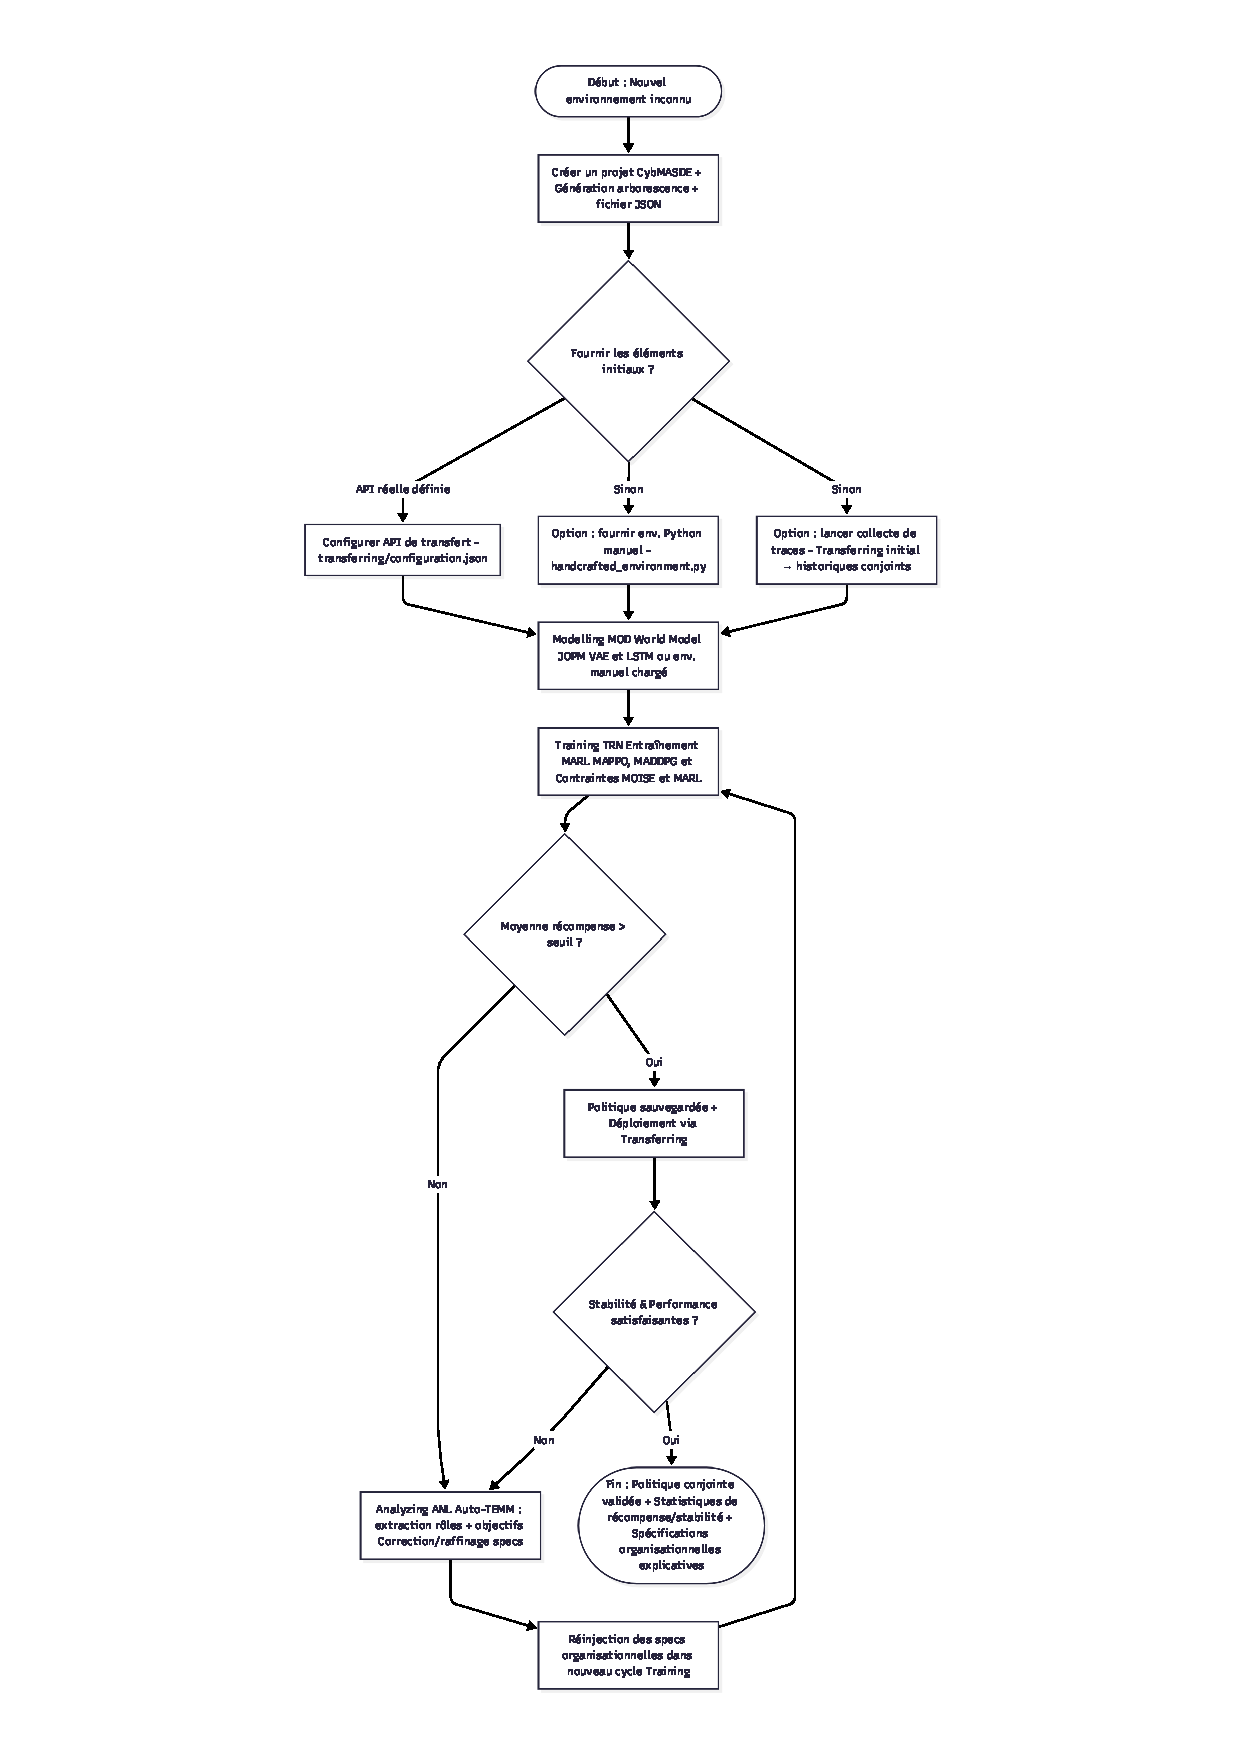
\includegraphics[trim={5cm 1cm 5cm 1cm},clip,height=\textheight]{figures/CybMASDE_user_flowchart.pdf}
  % }
  \caption{Cycle d’utilisation de CybMASDE}
  \label{fig:cybmasde_cycle}
\end{figure*}

\paragraph{1. Arrivée devant un nouvel environnement}
\begin{description}
  \item[Utilisateur :] Confronté à un nouvel environnement (ex.~: essaim de drones, réseau d’entreprise, architecture de microservices). Aucun modèle ni configuration n’existent encore.
  \item[CybMASDE :] Attend l’initialisation d’un projet pour orchestrer le cycle complet.
\end{description}

\paragraph{2. Création d’un projet}
\begin{description}
  \item[Utilisateur :] Crée un nouveau projet via l’interface. Une arborescence est générée avec les dossiers \texttt{modelling}, \texttt{training}, \texttt{analyzing}, \texttt{transferring}. Le fichier central \texttt{project\_configuration.json} est produit.
  \item[CybMASDE :] Génère les squelettes nécessaires (fichiers de configuration, API de transfert, gestionnaire d’espaces d’actions/observations). Cet espace devient le support du cycle \textbf{MTA+T} (Modelling, Training, Analyzing, Transferring).
\end{description}

\paragraph{3. Fourniture des éléments initiaux}
\begin{description}
  \item[Utilisateur :] Renseigne au moins une des options :
    \begin{enumerate}
      \item \textbf{API réelle} (\texttt{transferring/configuration.json}) si elle existe déjà.
      \item \textbf{Environnement Python manuel} (\texttt{handcrafted\_environment.py}).
      \item \textbf{Ensemble de traces collectées} par une précédente exécution d’une politique aléatoire afin de générer des historiques conjoints.
    \end{enumerate}
  \item[CybMASDE :] Vérifie la configuration. En cas de collecte de traces, sauvegarde les historiques dans \texttt{world\_model/traces}.
\end{description}

\begin{description}
  \item[Utilisateur :] Implémente la classe des fonctions composantes si aucun un environnement Python manuel n’est fourni :
    \begin{enumerate}
      \item \textbf{Fonction de récompense basée sur les historiques} en implémentant la méthode \texttt{reward()}.
      \item \textbf{Fonction d'arrêt basée sur les historiques} en implémentant la méthode \texttt{stop()}.
      \item \textbf{Fonction de rendu basée sur les historiques} en implémentant la méthode \texttt{render()}.
    \end{enumerate}
  \item[CybMASDE :] Vérifie la validité de la classe fournie et sauvegarde dans \texttt{generated\_environment/}.
\end{description}

\paragraph{4. Modelling (MOD)}
\begin{description}
  \item[Utilisateur :] Lance la génération d’un environnement simulé.
  \item[CybMASDE :]
    \begin{itemize}
      \item Si des traces sont présentes : entraîne un \textbf{Joint-Observation Prediction Model (JOPM)} basé sur PyTorch (VAE, MLP, LSTM optimisé par Adam).
      \item Si un environnement Python est fourni : le charge directement.
    \end{itemize}
    Le modèle simulé est stocké dans \texttt{generated\_environment/}.
\end{description}

\paragraph{5. Training (TRN)}
\begin{description}
  \item[Utilisateur :] Démarre l’entraînement des politiques multi-agents.
  \item[CybMASDE :] Utilise MARLlib (MAPPO, MADDPG, QMix, etc.) et Ray RLlib. Applique les contraintes \acn{MOISE+MARL} via masquage d’actions par rôle et shaping de récompenses. Les hyperparamètres (LR, $\gamma$, taille de batch, etc.) sont optimisés via Optuna. Sauvegarde checkpoints et statistiques dans \texttt{training/}.
\end{description}

\paragraph{6. Vérification de la récompense}
\begin{description}
  \item[Utilisateur :] Définit un seuil de performance (ex.~: $3.5\%$).
  \item[CybMASDE :] Compare la moyenne des récompenses au seuil. Si supérieur, sauvegarde la politique et passe au déploiement. Sinon, active l’étape d’analyse.
\end{description}

\paragraph{7. Analyzing (ANL)}
\begin{description}
  \item[Utilisateur :] Peut consulter les spécifications organisationnelles extraites et décider de les corriger ou de les injecter.
  \item[CybMASDE :] Exécute Auto-TEMM ou TEMM : clustering des trajectoires (DTW, LCS), inférence de rôles et objectifs, calcul d’adéquation organisationnelle (SOF + FOF). Les résultats sont sauvegardés dans \texttt{analyzing/}. Avec Auto-TEMM, les spécifications sont automatiquement déterminées sans que l'utilisateur ne puisse ajuster lui-même les hyperparamètres ce qui peut limiter la personnalisation.
\end{description}

\paragraph{8. Raffinement par itération}
\begin{description}
  \item[Utilisateur :] Relance l’entraînement avec les spécifications corrigées.
  \item[CybMASDE :] Réalise une boucle Analyse $\rightarrow$ Réinjection $\rightarrow$ Entraînement, jusqu’à atteindre le seuil ou un nombre maximal d’itérations. La meilleure politique est toujours conservée.
\end{description}

\paragraph{9. Transferring (TRF)}
\begin{description}
  \item[Utilisateur :] Déploie la politique validée dans l’environnement réel.
  \item[CybMASDE :] Assure le déploiement via deux modes :
    \begin{itemize}
      \item \textbf{REMOTE} : politique exécutée sur un serveur externe, les agents appliquent les actions reçues.
      \item \textbf{DIRECT} : politique embarquée dans les agents eux-mêmes.
    \end{itemize}
    Continue la collecte de traces et déclenche périodiquement de nouveaux cycles MTA.
\end{description}

\paragraph{10. Fin du processus}
\begin{description}
  \item[Utilisateur :] Obtient une politique conjointe validée, assortie de statistiques de performance et stabilité, et de spécifications organisationnelles explicatives.
  \item[CybMASDE :] Fournit un SMA complet, opérationnel et documenté, stockant tous les résultats dans l’arborescence du projet.
\end{description}

\medskip
En résumé, \acn{CybMASDE} automatise et structure la méthode \acn{MAMAD} à travers une chaîne modulaire \textbf{Modelling → Training → Analyzing → Transferring}, permettant à l’utilisateur de passer d’un environnement inconnu à un \acn{SMA} opérationnel, performant et explicable.


\begin{figure}
  \centering
  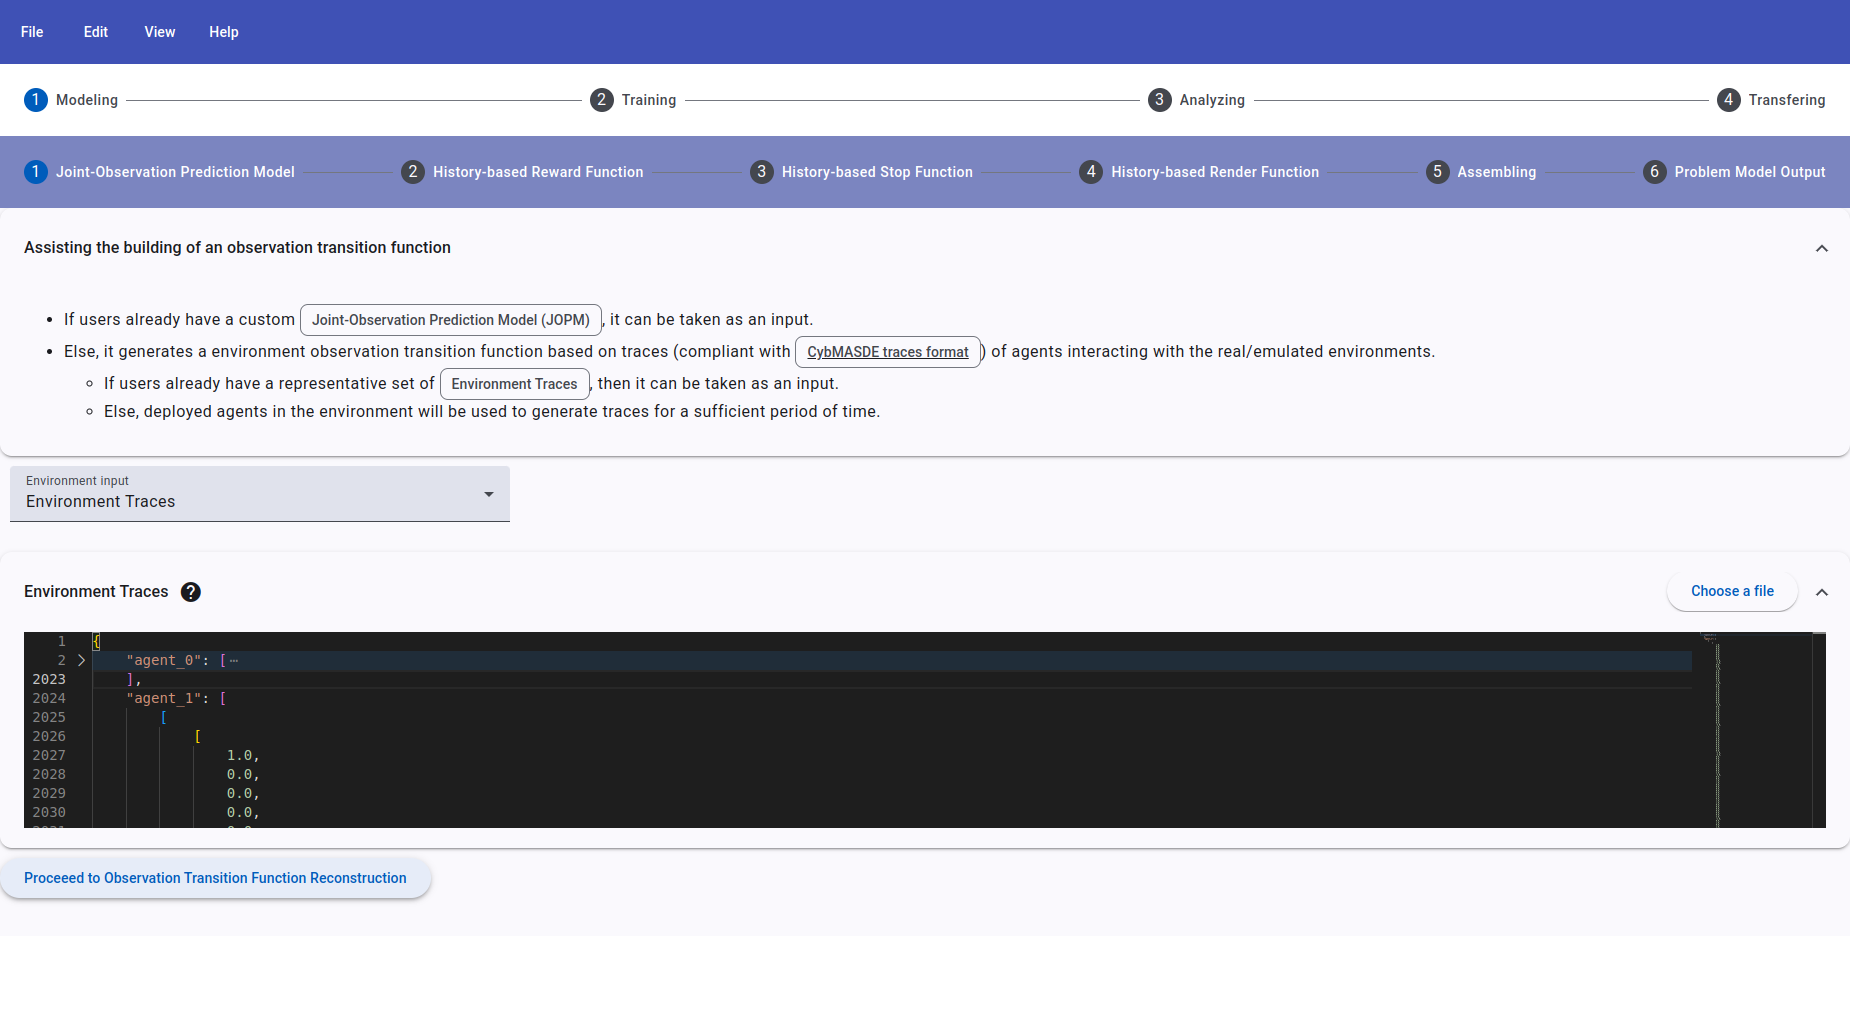
\includegraphics[width=\linewidth]{figures/CybMASDE_2.png}
  \caption{Captures d'écran de l'interface graphique de CybMASDE montrant l'onglet de modélisation}
  \label{fig:cybmasde_screenshot}
\end{figure}


\section*{Architecture logicielle et aspects de développement de \texttt{CybMASDE}}

\paragraph{Vue d’ensemble}
\texttt{CybMASDE}\footnotemark[1] est une plateforme modulaire et extensible destinée à la conception de systèmes multi-agents selon la méthode \acn{MAMAD}. Elle combine apprentissage (modélisation, entraînement), inférence organisationnelle et déploiement dans un environnement technologique cohérent. L'application est structurée autour d'un backend Python et d'une interface utilisateur, tous deux orchestrés via une API REST.

\footnotetext[1]{Code source et documentation disponible sur \url{https://github.com/julien6/CybMASDE}}


\subsection*{Stack technologique (développement)}

\begin{itemize}
  \item \textbf{Langage principal (backend)} : Python — intégrant des bibliothèques standards telles que \texttt{PyTorch}, \texttt{MARLlib}, \texttt{Ray RLlib}, \texttt{Optuna}, etc. Ce backend implémente entièrement les modules Modelling, Training, Analyzing et Transferring.
  \item \textbf{Interface utilisateur (frontend)} : développée avec Angular, elle offre une expérience graphique permettant à l’utilisateur de renseigner les paramètres d’un projet — notamment par glisser-déposer ou injection directe des fichiers d’historiques — sans manipuler l’arborescence de fichiers du projet.
  \item \textbf{API REST} : point d’intégration clé entre front-end, back-end et ligne de commande, garantissant une interface cohérente et réutilisable quel que soit le mode d’utilisation.
  \item \textbf{CLI (mode console)} : l’ensemble des fonctionnalités du backend est exposé via une interface en ligne de commande, utilisant la même API REST que le frontend.
\end{itemize}

L’architecture de CybMASDE démontre l’usage des frameworks et dépendances suivants :
\begin{itemize}
  \item \texttt{PyTorch} — entraînement des modèles VAE, LSTM (modélisation du monde simulé).
  \item \texttt{MARLlib} + \texttt{Ray RLlib} — apprentissage multi-agents avec une grande variété d'algorithmes comme MAPPO, QMix, MADDPG, etc.
  \item \texttt{Optuna} — optimisation des hyperparamètres (learning rate, discount factor, PPO clip value, etc.).
  \item \texttt{Angular} — développement de l’interface graphique.
  \item \texttt{Python 3.8 \& Angular v15} -- gestion des dépendances et environnement de développement.
\end{itemize}



\paragraph{Modularité et cycle de développement}
Le backend Python est organisé en modules correspondant aux étapes de la méthode MAMAD :
\textit{Modelling}, \textit{Training}, \textit{Analyzing}, \textit{Transferring}, chacun activable via l’API REST.
Cette modularité facilite la maintenance, l’extensibilité et les tests unitaires (ex. injecter un modèle, remplacer un algorithme d’entraînement, personnaliser l’analyse). L’interface Angular communique avec ces modules de manière unifiée.

\paragraph{Schéma conceptuel}
La \autoref{fig:cybmasde_uml} montre une vue \textit{composant C4} mettant en évidence les interactions entre :
\begin{itemize}
  \item \textsf{Frontend Angular} (UX interactive du projet),
  \item \textsf{Backend Python}, modules MTA+T,
  \item \textsf{API REST} comme couche d’interface commune,
  \item \textsf{Systèmes cibles} (environnements via PettingZoo ou APIs spécifiques).
\end{itemize}

\begin{figure}
  \centering
  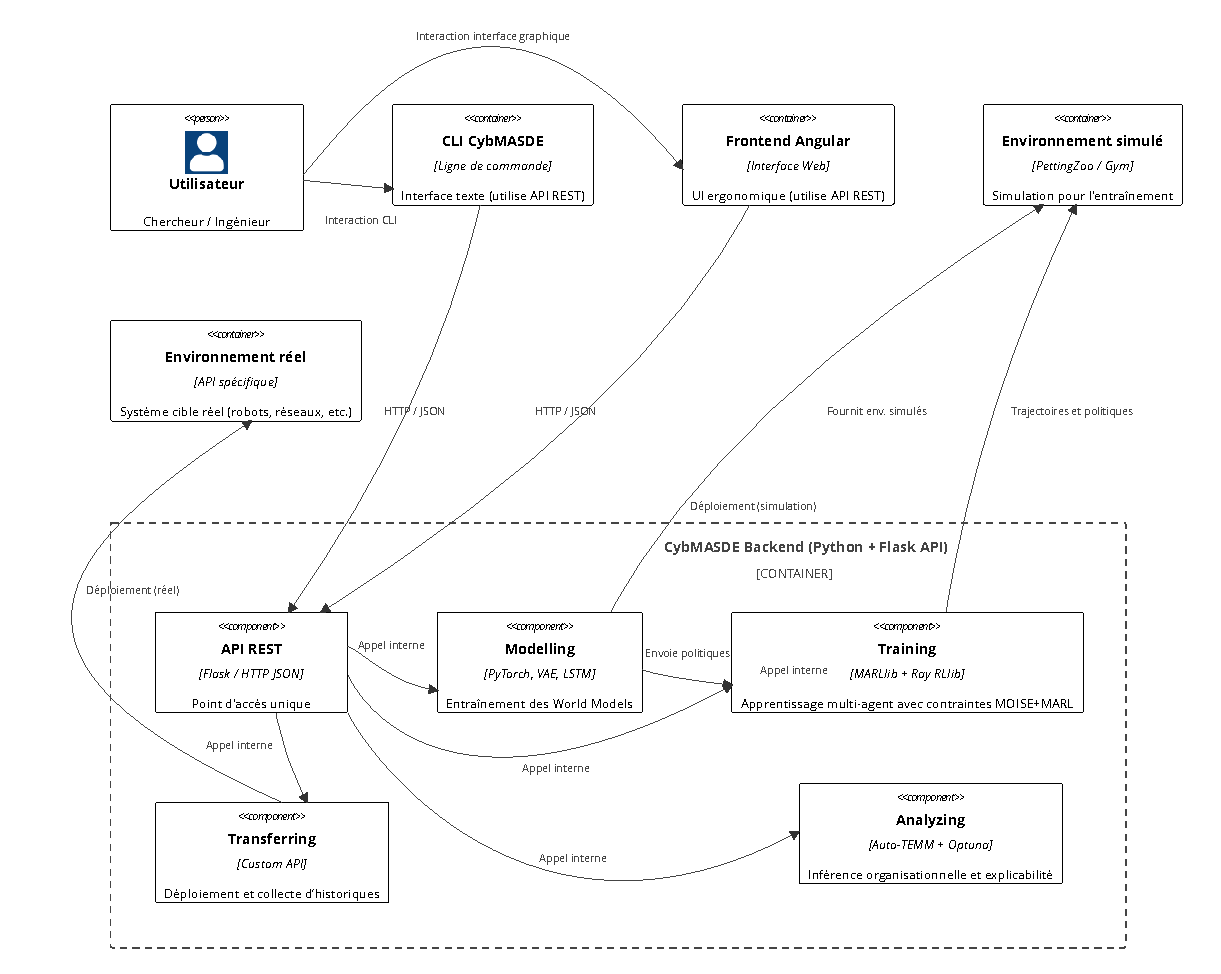
\includegraphics[trim={2.25cm 9cm 2.25cm 10cm},clip,width=0.8\textwidth]{figures/CybMASDE_internal_component_diagram.pdf}
  \caption{Diagramme de composants UML illustrant l'architecture logicielle de CybMASDE}
  \label{fig:cybmasde_uml}
\end{figure}

\section{Intégration des différentes contributions}

\subsection{Implémentation du modèle Dec-POMDP pré-spécialisé pour la Cyberdéfense}

En complément de la modélisation automatique basée sur des \textit{World Models}, nous proposons une approche de modélisation manuelle guidée par un modèle pré-spécialisé pour les environnements de cyberdéfense.
Le développement du formalisme \acn{Dec-POMDP} appliqué à ce domaine a conduit à un modèle que nous appelons \textbf{Multi-Cyberdefense Agent Simulator (MCAS)}. Celui-ci constitue une instance particulière de \acn{Dec-POMDP} adaptée aux scénarios de cyberdéfense (présentée en \autoref{fig:model_example_illustration}).

Une implémentation Python de ce modèle est fournie dès la création d’un projet dans le fichier
\textit{modelling/simulated\_environment/handcrafted\_environment.py}
Par défaut, ce fichier est un \textit{gabarit} à compléter. L’utilisateur doit y définir les composantes du modèle (espaces d’observations, espaces d’actions, dynamique de transition, fonction de récompense, fonction d’arrêt) en respectant le formalisme \acn{Dec-POMDP} et l’interface attendue par \acn{CybMASDE}.


Une fois complété, ce modèle est automatiquement intégré dans le cycle de \acn{CybMASDE} et peut être utilisé comme environnement de simulation pour l’entraînement multi-agent. L’exécution peut être réalisée en mode \textit{tour à tour}, permettant :
\begin{itemize}
  \item la visualisation en temps réel des propriétés de l’environnement et des agents,
  \item la représentation de l’environnement sous forme de graphe,
  \item l’affichage de métriques de suivi (récompenses, états, actions).
\end{itemize}
En complément du code Python, une représentation \texttt{JSON} du modèle est également possible. Elle permet de décrire :
\begin{itemize}
  \item les propriétés des nœuds et des actions de l’environnement,
  \item les agents définis et leurs comportements,
  \item les interactions globales du système.
\end{itemize}

\medskip
Ainsi, l'instance de simulation \textbf{MCAS} offre une alternative manuelle et structurée à la modélisation automatique, facilitant la construction d’environnements de simulation adaptés à des scénarios de cyberdéfense tout en restant compatible avec la chaîne MTA+T de \acn{CybMASDE}.

\subsection{Implémentation du framework MOISE+MARL}

Nous avons développé une implémentation du cadre MOISE+MARL appelée \textquote{MMA}~\hyperref[fn:github]{\footnotemark[2]} (API MOISE+MARL), qui est une API Python intégrant tous les ensembles et relations théoriques afin de minimiser les interactions avec l'utilisateur. MMA utilise une approche orientée objet, structurant le modèle $\mathcal{M}OISE^+$ en classes de données imbriquées, avec la classe « Moise » à la racine, permettant aux utilisateurs de définir des spécifications organisationnelles, telles que les rôles, les objectifs et les autorisations.

\footnotetext[2]{ \label{fn:github} L'implémentation \textquote{MOISE+MARL API} (MMA), les hyperparamètres et spécifications utillisés sont disponibles à \url{https://github.com/julien6/MOISE-MARL}.}

Pour prendre en charge les environnements Dec-POMDP, nous avons utilisé la bibliothèque \textit{PettingZoo} \cite{terry2020pettingzoo}, qui fournit une API standard pour les systèmes multi-agents et garantit l'interopérabilité entre différents environnements, à l'instar du framework Gymnasium \cite{kwiatkowski2024}. MMA intègre un dictionnaire pour le mappage des étiquettes d'observation/action ($l$), que les utilisateurs peuvent personnaliser, et prend également en charge les modèles de trajectoire \acn{TP} pour faciliter la définition et la correspondance des modèles.

Chaque type de guide de contrainte, comme $rag$, $rrg$ et $grg$, est implémenté dans une classe distincte. Les utilisateurs peuvent définir ces guides à l'aide de fonctions personnalisées ou de règles JSON~; par exemple, $rag$ peut être instancié en associant une paire $\langle \text{TP, dernière observation} \rangle$ aux actions attendues, tandis que $grg$ peut appliquer des bonus en fonction de TP spécifiques. La classe globale « MMA » intègre ces guides avec des relations définies par l'utilisateur, telles que la liaison d'un agent à un rôle ($ar$) ou l'association d'un rôle à $rrg$ et $rag$, en incorporant les spécifications organisationnelles définies dans la structure $\mathcal{M}OISE^+$.

Une fois configuré, l'objet MMA est utilisé pour encapsuler l'environnement avec un wrapper \textit{PettingZoo}. Ce wrapper applique des masques d'action et modifie les récompenses à chaque étape, garantissant que les agents respectent les spécifications organisationnelles tout au long de la formation. MMA intègre également \textit{MARLlib} \cite{hu2021marlib}, qui donne accès à des algorithmes MARL de pointe, permettant ainsi d'exécuter l'entraînement sur un cluster informatique haute performance.

Après l'entraînement, la méthode TEMM est utilisée, en utilisant des hyperparamètres optimisés manuellement pour déduire les rôles et les objectifs implicites grâce à un regroupement hiérarchique et à la méthode K-means. Cette analyse génère des résultats visuels, tels que des dendrogrammes pour les rôles et des graphiques de transition d'observation conjointe pour les objectifs. Les rôles et les objectifs implicites qui en résultent peuvent être exportés sous forme de trajectoires JSON, offrant une vue structurée des comportements organisationnels déduits.

\section*{Bilan}

Ce chapitre a présenté les outils d'expérimentation de la méthode \acn{MAMAD} au travers de sa mise en œuvre dans \acn{CybMASDE}, un outil permettant d'appliquer de façon flexible la méthode sur divers scénarios. Le chapitre suivant propose d'utiliser cet outil pour définir un cadre expérimental générique, applicable à tous les cas d'étude présentés dans le \autoref{chap:case_studies}.


\clearpage
\thispagestyle{empty}
\null
\newpage

\chapter{Cadre expérimental et d'évaluation}
\label{chap:cadre_experimental}

Le but de ce chapitre est de définir un cadre expérimental générique, applicable à tous les cas d'étude présentés dans le \autoref{chap:case_studies}. L'objectif est de fournir un \textit{canevas} que chaque scénario peut instancier en précisant les éléments choisis de la méthode MAMAD. Ce cadre s'appuie sur la méthode \acn{MAMAD}, la taxonomie des activités et sous-activités présentée en \autoref{tab:mamad_taxonomy}, et les critères d'évaluation définis précédemment.

\section{Description des ensembles d'environnements et algorithmes considérés}

Pour garantir la généralité et la robustesse de l’évaluation, nous considérons un ensemble varié d’environnements de référence issus de la littérature MARL~:
\begin{itemize}
  \item \textbf{Overcooked-AI}~\cite{overcookedai}: environnement de type jouet coopératif complexe nécessitant coordination et planification séquentielle.
  \item \textbf{Proie-Prédateur}~\cite{lowe2017multi}: environnement  de type jouet de poursuite-évasion, utilisé pour tester la coordination et la compétition.
  \item \textbf{Warehouse Management} : un environnement  de type jouet original que nous avons proposé pour simuler la gestion logistique multi-agent avec contraintes de flux et de ressources.
  \item \textbf{Company infrastructure}~\cite{cyberbattlesim}: une simulation d’attaques et de défenses sur un réseau, inspirée de MITRE ATT\&CK.
  \item \textbf{Drone Swarm}~\cite{cage_challenge_3_announcement}: une simulation d'un essaim de drones soumis à des attaques logicielles et nécessitant une défense collective.
  \item \textbf{Microservices Kubernetes} : un environnement réel constitué d'un cluster de quatres micro-services interconnectés et que nous avons proposé pour l'orchestration de microservices avec auto-scaling et résilience face à des défaillances intentionelles.
\end{itemize}

L’environnement \textbf{Microservices Kubernetes} se distingue des autres par sa nature réelle : il s’agit d’un système de quatre services interconnectés, alors que les autres environnements sont simulés. Pour des raisons pratiques, l’environnement simulé sert de référence << réelle >>, ce qui permet d’appliquer \acn{MAMAD} comme sur un système opérationnel, le \textit{World Model} jouant ici le rôle d’une simulation de la simulation. Ce choix valide le principe de \acn{MAMAD} : si le \textit{World Model} reconstruit à partir de traces est suffisamment fidèle, les politiques apprises peuvent être transférées efficacement, facilitant ainsi la comparaison entre simulation et réalité. Dans ce scénario, l’environnement \textbf{Microservices Kubernetes} est directement exploitable avec \acn{MAMAD} sans nécessiter de modélisation supplémentaire, et le transfert (\acn{TRF}) s’effectue vers ce système réel, démontrant la validité de l’approche dans un contexte opérationnel.

\medskip

Les algorithmes MARL sélectionnés couvrent les principales familles reconnues dans la littérature~:
\begin{itemize}
  \item \textbf{MAPPO} (Multi-Agent Proximal Policy Optimization)~\cite{Yu2022}
  \item \textbf{MADDPG} (Multi-Agent Deep Deterministic Policy Gradient)~\cite{lowe2017multi}
  \item \textbf{QMIX}~\cite{rashid2018qmix}
  \item \textbf{COMA}~\cite{foerster2018counterfactual}
  \item \textbf{IQL} (Independent Q-Learning)~\cite{Jiang2022}
  \item \textbf{VDN} (Value Decomposition Networks)~\cite{sunehag2018value}
\end{itemize}
Les environnements sont implémentés via \textit{PettingZoo}~\cite{terry2020pettingzoo} et les algorithmes via \textit{MARLlib}~\cite{hu2022marllib}.

\section{Conditions de reproductibilité}

\subsection{Conditions expérimentales matérielles}
\label{par:compute_conditions}
Les expériences sont réalisées sur un \textbf{cluster HPC académique}. Sauf mention contraire, les constantes suivantes s’appliquent à tous les scénarios~:
\begin{itemize}
  \item \textbf{Accélérateurs}~: NVIDIA A100 / V100, AMD MI210.
  \item \textbf{Frameworks DL}~: PyTorch~\cite{Paszke2019} et TensorFlow~\cite{Abadi2016} (implémentations MARLlib/MAPPO, etc.).
  \item \textbf{Optimisation d’hyperparamètres}~: \textbf{Optuna}~\cite{akiba2019optuna} (TPE) pour LR, exploration/exploitation, tailles de réseaux ; espace de recherche standardisé par famille d’algorithmes.
  \item \textbf{Parallélisme}~: $\sim$ 5 exécutions indépendantes par condition (algorithme $\times$ environnement $\times$ contrainte).
  \item \textbf{OS et libs}~: Linux 64-bit, CUDA/cuDNN ou ROCm selon GPU ; environnements figés (conda/pip).
\end{itemize}
Les études de cas ne rappellent que les \textbf{déviations spécifiques} (ex. nombre de runs, GPU particulier).

\subsection{Gestion des hyperparamètres (par défaut et surcharges)}
Chaque couple \{algorithme, environnement\} est initialisé avec un \textit{profil standard} issu de MARLlib et d’expériences préliminaires.
Une passe d’HPO contrôlée peut être réalisée avec \textbf{Optuna} (budget borné, mêmes priorités d’espace de recherche entre scénarios)~\cite{akiba2019optuna}. Le meilleur \textit{trial} est ensuite \textbf{rejoué 5 fois} pour agrégation des résultats.
Les scénarios peuvent :
\begin{enumerate}[label=\alph*)]
  \item accepter les valeurs par défaut,
  \item restreindre l’HPO,
  \item surcharger explicitement certains hyperparamètres.
\end{enumerate}

\section{Baselines expérimentales}

Une baseline expérimentale est un ensemble de données qui servent à la reproduction de l'experimentation. Dans notre cas, une baseline inclue~:
\begin{itemize}
  \item \textbf{Activités} : Une sélection d'activités MAMAD (MOD, TRN, ANL, TRF et leurs variantes : AUT, MAN, CON, UNC, etc.).
  \item \textbf{Algorithme} : Un algorithme MARL (MAPPO, QMIX, MADDPG, etc.) ou un autre algorithme issu de la littérature susceptible de permettre aux agents d'atteindre leurs objectifs avec une autre approche.
  \item \textbf{Spécifications organisationnelles} : Un ensemble de spécifications organisationnelles de type MOISE+MARL (rôles et missions) si l'algorithme choisi appartient au domaine du \acn{MARL}.
  \item \textbf{Environnement} : Un environnement avec variantes des scénarios (ex. Overcooked-AI~\cite{overcookedai}, Proie-Prédateur~\cite{lowe2017multi}, Drone Swarm~\cite{cage_challenge_3_announcement}).
  \item \textbf{Métriques spécifiques} : Un ensemble de métriques spécifiques à l'environnement ou l'étude (spécifiques à l’environnement).
  \item \textbf{Conditions d’exécution} : Un ensemble de conditions d’exécution (nb de runs, seeds, matériel, perturbations éventuelles).
\end{itemize}

Chaque baseline peut être représentée sous forme tabulaire en précisant ces éléments pour assurer la comparabilité et la reproductibilité. L'interêt d'établir des baselines est de fournir des points de référence clairs pour évaluer l'impact des différentes composantes de la méthode MAMAD. En comparant les performances obtenues avec ces baselines, il devient possible d'identifier les contributions spécifiques de chaque activité (modélisation, entraînement, analyse, transfert) ainsi que l'effet des spécifications organisationnelles sur le comportement et l'efficacité du système multi-agent.

\section{Grille d’évaluation}

\subsection{Critères et métriques associées}
L’évaluation s’appuie sur une grille de critères inspirée des recommandations de la communauté RL/MARL~\cite{papoudakis2021agent} :

\begin{table}[h!]
  \centering
  \caption{Correspondance entre critères globaux et métriques}
  \begin{tabular}{|l|l|}
    \hline
    \textbf{Critère}   & \textbf{Métriques associées}                                       \\
    \hline
    C1 – Autonomie     & Proportion d’intervention (conception / fonctionnement)            \\
    \hline
    C2 – Performance   & Récompense cumulée ; Taux de convergence                           \\
    \hline
    C3 – Adaptation    & Écart-type des récompenses ; Score de robustesse                   \\
    \hline
    C4 – Contrôle      & Taux de violation des contraintes ; Score de cohérence             \\
    \hline
    C5 – Explicabilité & Adéquation organisationnelle ; Qualité des spécifications inférées \\
    \hline
  \end{tabular}
  \label{tab:grille}
\end{table}

Ces différentes métriques visent à déterminer dans quelle mesure les cinq critères globaux (C1--C5) sont couverts sur une baseline donnée.
Chaque métrique est décrite séparément pour plus de clarté.

\paragraph{Proportion d’intervention (conception / fonctionnement).}
\textit{Unité : pourcentage (\%). Source : logs d’utilisation de la plateforme, questionnaires utilisateurs, scripts d’automatisation.}
Elle est calculée comme suit :
\[
  \frac{\text{nombre d’actions nécessitant une intervention humaine}}{\text{nombre total d’actions}} \times 100.
\]
Cette proportion peut être mesurée automatiquement via l’instrumentation logicielle (nombre de cycles de raffinement) ou manuellement par annotation des étapes.

\paragraph{Récompense cumulée.}
\textit{Unité : valeur numérique sans unité (souvent normalisée). Source : logs d’entraînement MARLlib/RLlib, fichiers de résultats d’épisodes.}
Il s’agit de la somme des récompenses obtenues par tous les agents sur un épisode ou sur une fenêtre glissante.
Elle est extraite automatiquement via des scripts d’analyse.

\paragraph{Taux de convergence.}
\textit{Unité : nombre d’épisodes (entier). Source : courbes d’apprentissage, logs d’entraînement.}
Il correspond au nombre d’épisodes nécessaires pour que la moyenne des récompenses dépasse un seuil prédéfini et reste stable.
Le calcul est automatisé par détection de plateau sur la courbe d’apprentissage.

\paragraph{Écart-type des récompenses.}
\textit{Unité : identique à la récompense (souvent sans unité). Source : logs d’entraînement, résultats de runs multiples.}
Cette métrique correspond à l’écart-type statistique des récompenses moyennes entre plusieurs runs indépendants.
Elle est calculée automatiquement lors de l’agrégation des résultats.

\paragraph{Score de robustesse.}
\textit{Unité : ratio ou pourcentage (\%). Source : tests sous perturbations (pannes, attaques), logs d’épisodes.}
Il se définit comme :
\[
  \frac{\text{performance sous perturbation}}{\text{performance nominale}}
  \quad \text{ou} \quad
  \frac{\text{nombre d’épisodes avec performance > seuil}}{\text{nombre total d’épisodes}}.
\]
Ce score est obtenu en comparant les performances moyennes dans des scénarios perturbés et des scénarios de référence.
Les perturbations sont générées soit par des seeds différentes dans les environnements simulés, soit par des changements explicites (topologie, pannes, attaques, etc.).

\paragraph{Taux de violation des contraintes.}
\textit{Unité : pourcentage (\%). Source : logs d’exécution, wrappers d’environnement, analyse post-hoc.}
La formule est :
\[
  \frac{\text{nombre de violations détectées}}{\text{nombre total d’actions ou d’épisodes}} \times 100.
\]
Cette mesure évalue la capacité des agents à respecter les règles imposées par leurs rôles.
Elle varie avec la dureté des contraintes : un taux nul est attendu lorsque la dureté est maximale, et un taux élevé lorsque les contraintes sont nulles.
Les valeurs intermédiaires doivent être analysées en lien avec la récompense cumulée afin d’identifier d’éventuelles règles trop contraignantes qui réduiraient les performances globales.

\paragraph{Score de cohérence.}
\textit{Unité : ratio (0–1) ou pourcentage (\%). Source : clustering des trajectoires, analyse TEMM/Auto-TEMM.}
Ce score mesure la similarité entre les comportements observés et les rôles attendus (pureté de clusters, F1-score).
L’idée est de comparer les spécifications organisationnelles originales avec celles inférées automatiquement.
Plus la distance entre les deux ensembles de trajectoires est faible, plus le score de cohérence est élevé, indiquant une bonne prise en compte des spécifications organisationnelles par MOISE+MARL et une capacité d’inférence fiable de TEMM/Auto-TEMM.

\paragraph{Adéquation organisationnelle.}
\textit{Unité : ratio (0–1). Source : analyse TEMM, matrices de correspondance rôles-missions.}
Elle est calculée comme une moyenne pondérée des scores structurels (SOF) et fonctionnels (FOF) :
\[
  \text{OF} = \alpha \cdot \text{SOF} + (1-\alpha) \cdot \text{FOF}.
\]
Cette mesure quantifie à quel point les politiques apprises respectent la structure organisationnelle attendue.

\paragraph{Qualité des spécifications inférées.}
\textit{Unité : pourcentage (\%) ou score de similarité. Source : comparaison automatique entre spécifications inférées (JSON, TEMM) et spécifications de référence.}
Cette métrique mesure la qualité des spécifications organisationnelles inférées en comparant leur similarité avec les spécifications de référence, à l’aide d’indicateurs tels que l’indice de Jaccard ou la distance Euclidienne. Contrairement au score de cohérence, elle s’intéresse uniquement à la fidélité des spécifications extraites, indépendamment des politiques apprises. Le calcul repose sur une comparaison systématique entre les spécifications inférées et les spécifications initiales, en variant les scénarios pour évaluer la capacité de généralisation. L’objectif est de trouver un compromis entre la fidélité aux spécifications de départ et la capacité de généralisation, en évitant le surapprentissage et en limitant la complexité des règles ou objectifs inférés, tout en maximisant la similarité avec les trajectoires de référence.

\section{Protocole d'expérimentation et d'évaluation}\label{sec:protocole_experimental}

Le protocole expérimental proposé suit un raisonnement progressif semblable aux pratiques de la communauté~\cite{papoudakis2021agent}.
L'ensemble des étapes 1 à 4 constitue le protocole d'experimentation tandis que les étapes 5 et 6 concernent l'évaluation des résultats :

\paragraph{1. Configuration initiale}
Configuration requise incluant la mise en place de l’API REST de communication avec l'environnement et les différentes composantes requises pour modéliser l'environnement et autres données nécéssaires pour créer un projet CybMASDE pour une baseline donnée.

\paragraph{2. Mise en place de la baseline avancée}
Définition d’au moins une \textbf{baseline avancée} considérée comme la \textbf{baseline par défaut} :
\begin{table}[h!]
  \centering
  \caption{Caractérisation générique de la \textquote{baseline avancée}}
  \label{tab:baseline_generic}
  \renewcommand{\arraystretch}{1.2}
  \footnotesize
  \begin{tabular}{p{4.8cm}p{9cm}}
    \hline
    \textbf{Élément}                  & \textbf{Valeur instanciée}                                                                                                      \\
    \hline
    Environnement                     & Nom de l’environnement et éventuelles variantes de scénarios (ex.~Overcooked-AI, layout classique).                             \\ \hline
    Activités MAMAD                   & \textquote{MOD-AUT,TRN-CON,ANL-AUT,TRF-AUT}                                                                                     \\ \hline
    Algorithme                        & Algorithme sélectionné avec son implémentation (ex.~MAPPO via MARLlib).                                                         \\ \hline
    Spécifications organisationnelles & Ensemble MOISE+MARL contenant à la fois des rôles et des missions.                                                              \\ \hline
    Métriques spécifiques             & Indicateurs complémentaires propres à l’environnement (ex.~plats servis, taux de collisions, drones infectés, latence moyenne). \\ \hline
    Conditions d’exécution            & Nb de runs, seeds, type de matériel (CPU/GPU), perturbations/stress-tests.                                                      \\ \hline
  \end{tabular}
\end{table}

\paragraph{3. Mises en place de baselines alternatives}
Definition possible d'autres baselines jouant sur d'autres paramètres tels que les algorithmes MARL, les contraintes organisationnelles ou la modélisation en fonction des questions spécifiques de chaque scénario. Des base

\paragraph{4. Définition d’études d’ablation}
Réalisation d’au moins une \textbf{étude d’ablation} : chaque ablation consiste prendre la \textbf{baseline avancée} et à changer un ou plusieurs paramètres notamment à remplacer une ou plusieurs activités MAMAD par des variantes moins avancées (par exemple, \texttt{ANL-MAN} en utilisant TEMM plutôt que Auto-TEMM, ou \texttt{TRN-UNC} sans contraintes organisationnelles) mais aussi à supprimer les contraintes organisationnelles, à changer d’algorithme, etc. Chaque ablation doit être justifiée en fonction des questions spécifiques de chaque scénario.

\paragraph{5. Comparaison et validation}
Comparaison systématique des résultats sur la grille d’évaluation (\autoref{tab:grille}) pour mesurer l’impact de chaque composant sur les critères cibles. L'analyse des résultats doit inclure des visualisations (courbes d’apprentissage, heatmaps, dendrogrammes, etc.) et une discussion critique des compromis observés (ex. performance vs. respect des contraintes).

\paragraph{6. Répétition et agrégation}
Répétition des expériences (5 runs indépendants, seeds consignées), agrégation statistique (moyenne, écart-type), et tests statistiques (t-test ou non paramétrique selon la normalité).


\section*{Bilan}

Ce cadre expérimental fournit une base reproductible pour l’évaluation de la méthode \acn{MAMAD} dans des contextes variés. Il garantit la comparabilité entre scénarios, la robustesse des résultats et la traçabilité des choix méthodologiques. Les chapitres suivants instancient ce cadre sur différents environnements, analysent les résultats obtenus et discutent la couverture des critères d’évaluation par la méthode proposée.


\clearpage
\thispagestyle{empty}
\null
\newpage


\chapter{Études de cas}
\label{chap:case_studies}

Ce chapitre présente les études de cas réalisées pour évaluer la méthode \acn{MAMAD} dans divers contextes. Chaque section détaille l'instanciation du cadre expérimental défini au \autoref{chap:cadre_experimental} pour un environnement spécifique, en précisant les choix méthodologiques et les configurations expérimentales.

\section{Description des expérimentations sur les environnements non-orientés Cyberdéfense}

Dans cette section, nous décrivons les expérimentations qui ont été menées sur un ensemble d'environnements de référence non orientés Cyberdéfense. L'objectif principal est de valider la méthode \acn{MAMAD} dans des contextes variés, en mettant l'accent sur la coordination, la compétition, et la gestion de ressources dans des environnements à observation partielle. Le but est d'avoir une preuve de concept que la méthode MAMAD est applicable sur des cas simples. A partir de là, il est possible d'aborder efficacement son application à des scénarios strictement liés à la cyberdéfense.

Cette section propose la même instance du protocole d'expérimentation de la \autoref{sec:protocole_experimental} (étapes 1 à 4) pour trois environnements non-orientés Cyberdéfense (\textit{Overcooked-AI}, \textit{Proie-Prédateur}, \textit{Warehouse Management}).
L’objectif est de décrire les expérimentations à mener pour appliquer le protocole d'évaluation de la \autoref{sec:protocole_experimental} (étape 5 à 6) dans le chapitre suivant afin de valider la méthode \acn{MAMAD} sur des contextes coopératifs/compétitifs variés, avec observation partielle et besoins de coordination.


\subsection{Description des environnements}

\subsubsection*{Overcooked-AI}

L'environnement \textbf{Overcooked-AI}~\cite{Carroll2019} simule un scénario de cuisine coopérative où les agents doivent collaborer pour préparer et servir des repas dans une cuisine structurée. Cet environnement est illustré dans \autoref{fig:overcooked}.

\begin{enumerate*}[label={\roman*)}, itemjoin={; \quad}]
  \item \textbf{Espace d'état :} Une cuisine discrète basée sur une grille avec des postes de travail (planche à découper, cuisinière, comptoir de service), des ingrédients et des agents
  \item \textbf{Espace d'observation :} Les agents observent les éléments de la cuisine dans un rayon défini
  \item \textbf{Espace d'action :}
  \begin{enumerate*}[label={\roman*)}, itemjoin={; \quad}]
    \item Déplacement : \texttt{Haut, Bas, Gauche, Droite}
    \item Interagir : \texttt{Choisir un ingrédient, couper, cuisiner, servir}.
  \end{enumerate*}
  \item \textbf{Structure de récompense :}
  \begin{enumerate*}[label={\roman*)}, itemjoin={; \quad}]
    \item Préparation réussie du repas : $+20$
    \item Mauvaise utilisation des ingrédients : $-5$
    \item Comportement passif : $-1$ par étape sans action significative.
  \end{enumerate*}
  \item \textbf{objectif :} Maximiser le nombre de commandes de repas terminées dans un délai fixe.
\end{enumerate*}
%
\textbf{Spécifications organisationnelles :}
\begin{enumerate*}[label={\roman*)}, itemjoin={; \quad}]
  \item \textbf{Rôles :} \texttt{Chef, assistant, serveur}
  \item \textbf{Missions :} Le chef prépare les plats, l'assistant fournit les ingrédients et le serveur sert les repas
  \item \textbf{Contraintes :} L'exécution des tâches doit être synchronisée afin d'éviter les goulots d'étranglement.
\end{enumerate*}

\begin{figure}[h!]
  \centering
  
\includegraphics[trim=0cm -0.5cm 0cm -0.5cm, clip, width=0.6\linewidth]{figures/overcooked.png}
  \caption{Capture d'écran de l'environnement Overcooked-AI : deux agents (chefs cuisiniers) doivent collaborer pour préparer et servir efficacement des soupes à l'oignon. Le processus consiste à prélever trois oignons (un à la fois) dans le distributeur, à les placer dans une marmite, à attendre que la soupe cuise, à récupérer un plat propre, à dresser la soupe et à la livrer au comptoir de service. La disposition de la cuisine comprend des obstacles et des passages étroits, ce qui oblige les agents à coordonner leurs mouvements pour éviter les collisions et optimiser l'accomplissement des tâches.}
  \label{fig:overcooked}
\end{figure}

\subsubsection*{Proie-Prédateur}

L'environnement \textbf{Proie-Prédateur} est un benchmark MARL bien connu~\cite{lowe2017multi}, conçu pour évaluer la coordination entre des poursuivants coopératifs (prédateurs) qui tentent de capturer un agent insaisissable (proie). Cet environnement est illustré dans \autoref{fig:predator_prey}.
%
\begin{enumerate*}[label={\roman*)}, itemjoin={; \quad}]
  \item \textbf{Espace d'état :} Un espace 2D continu où les agents (prédateurs et proies) ont des positions $(x, y)$ et des vitesses
  \item \textbf{Espace d'observation :} Les agents détectent les entités proches dans un rayon limité $r$
  \item \textbf{Espace d'action :}
  \begin{enumerate*}[label={\roman*)}, itemjoin={; \quad}]
    \item Déplacement : \texttt{Haut, Bas, Gauche, Droite, Rester sur place}.
  \end{enumerate*}
  \item \textbf{Structure de récompense :}
  \begin{enumerate*}[label={\roman*)}, itemjoin={; \quad}]
    \item Les prédateurs gagnent $+50$ pour chaque proie capturée
    \item La proie gagne $+1$ par étape de temps survécue ;.
  \end{enumerate*}
  \item \textbf{objectif :} Les prédateurs doivent coopérer pour piéger la proie, tandis que celle-ci tente de s'échapper aussi longtemps que possible.
\end{enumerate*}
%
\textbf{Spécifications organisationnelles :}
\begin{enumerate*}[label={\roman*)}, itemjoin={; \quad}]
  \item \textbf{Rôles :} \texttt{Prédateur, Proie}
  \item \textbf{Missions :} Les prédateurs coordonnent leurs efforts pour encercler la proie ; la proie cherche les meilleurs chemins pour s'échapper
  \item \textbf{Contraintes :} Les prédateurs doivent trouver un équilibre entre poursuite agressive et stratégies de blocage.
\end{enumerate*}
%
\begin{figure}[h!]
  \centering
  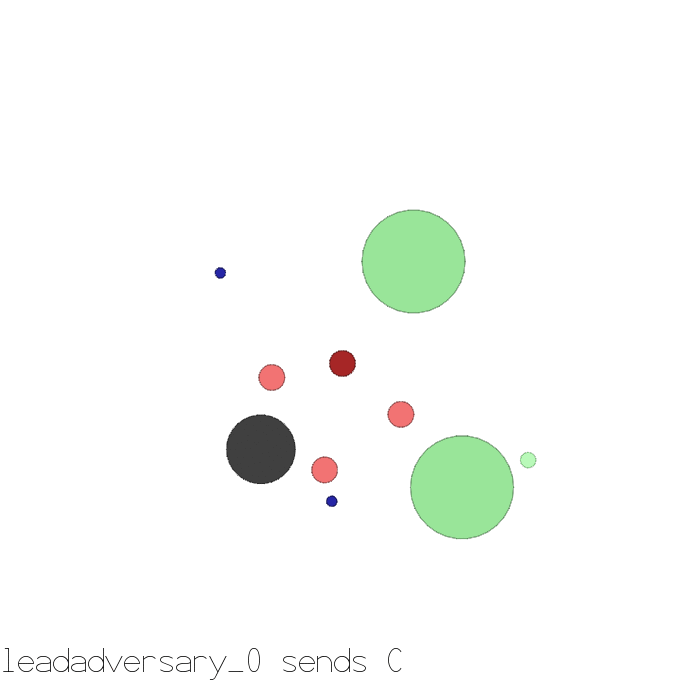
\includegraphics[trim=0cm 4.5cm 0cm 1cm, clip,width=0.6\linewidth]{figures/predator_prey.png}
  \caption{Capture d'écran de l'environnement Proie-Prédateur : \textbf{agents verts} (coopératifs) et \textbf{agents rouges} (adversaires). Les agents verts ont pour objectif de collecter les aliments dispersés dans l'environnement tout en évitant d'être détectés par les agents rouges. L'environnement comprend des \textbf{zones forestières} qui offrent un abri ; lorsqu'un agent vert pénètre dans une forêt, il devient partiellement ou totalement invisible aux yeux des agents rouges. Un agent rouge agit en tant que \textbf{chef} avec des capacités d'observation améliorées et peut communiquer avec les autres agents rouges afin de coordonner leur poursuite.}
  \label{fig:predator_prey}
\end{figure}

\subsubsection*{Warehouse Management}

L'environnement \textbf{Warehouse Management}~\cite{warehouse_management} modélise un entrepôt logistique basé sur une grille où plusieurs robots doivent collaborer pour transporter efficacement les marchandises. Cet environnement s'inspire des scénarios d'automatisation des entrepôts industriels et constitue un banc d'essai idéal pour évaluer la répartition des tâches, la spécialisation des rôles et la coordination en temps réel. Cet environnement est illustré dans \autoref{fig:warehouse}.
%
\begin{enumerate*}[label={\roman*)}, itemjoin={; \quad}]
  \item \textbf{Espace d'état :} Une grille $N \times M$ où chaque cellule contient un robot, un produit, une machine de fabrication ou un lieu de dépôt. Le système suit les positions des agents, les niveaux de stock et les états des machines
  \item \textbf{Espace d'observation :} Chaque agent dispose d'une vue locale $V \times V$, lui permettant de percevoir les produits, ses coéquipiers et les machines à proximité
  \item \textbf{Espace d'action :}
  \begin{enumerate*}[label={\roman*)}, itemjoin={; \quad}]
    \item Déplacement : \texttt{Haut, Bas, Gauche, Droite}
    \item Interagir : \texttt{Prendre un produit, déposer un produit}.
  \end{enumerate*}
  \item \textbf{Structure de récompense :}
  \begin{enumerate*}[label={\roman*)}, itemjoin={; \quad}]
    \item Livraison réussie du produit : $+10$
    \item Déplacement inefficace : $-1$ par étape inutile
    \item Mauvaise manipulation du produit : $-5$ pour les livraisons incorrectes.
  \end{enumerate*}
  \item \textbf{objectif :} Transporter les matières premières vers les machines de transformation et livrer les produits finis aux lieux de livraison.
\end{enumerate*}
%
\textbf{Spécifications organisationnelles :}
\begin{enumerate*}[label={\roman*)}, itemjoin={; \quad}]
  \item \textbf{Rôles :} \texttt{Transporteur, gestionnaire des stocks}
  \item \textbf{Missions :} Les transporteurs acheminent les produits, tandis que les gestionnaires des stocks supervisent les niveaux des stocks
  \item \textbf{Contraintes :} Les transporteurs doivent donner la priorité aux livraisons essentielles.
\end{enumerate*}

\begin{figure}[h!]
  \centering
  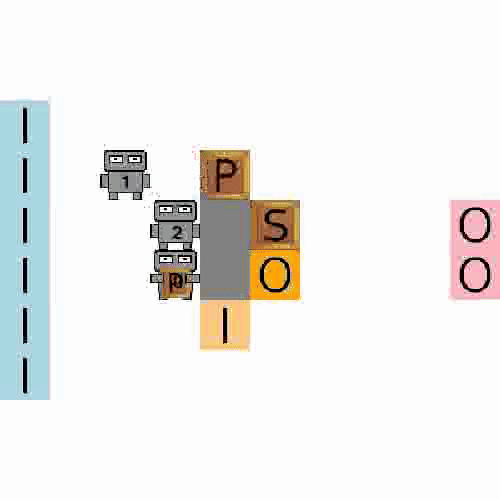
\includegraphics[trim=0cm 3cm 0cm 3cm, clip, width=0.6\linewidth]{figures/wm.png}
  \caption{Capture d'écran de l'environnement de Warehouse Management : les agents peuvent se déplacer vers le haut, le bas, la gauche et la droite. Plusieurs agents opèrent au sein d'une grille d'entrepôt, effectuant des tâches pour traiter et livrer des produits. Les agents peuvent se déplacer dans quatre directions (haut, bas, gauche, droite) et interagir avec les zones de prélèvement/dépôt lorsqu'ils sont adjacents. Le flux de travail comprend : (i) la collecte des produits primaires dans les zones de prélèvement/dépôt du convoyeur d'entrée (zones bleues) ; (ii) leur transport vers les zones de prélèvement/dépôt des machines de fabrication (zones marron), où les produits primaires sont transformés en un seul produit secondaire selon un schéma de fabrication prédéfini ; (iii) la récupération des produits secondaires obtenus et leur livraison aux zones de prélèvement/dépôt du convoyeur de sortie (zones roses). Pour que l'opération soit réussie, les agents doivent coordonner leurs mouvements et leurs actions afin d'optimiser le débit et l'efficacité au sein de l'entrepôt.}
  \label{fig:warehouse}
\end{figure}


\subsection{Description de l'instance commune du protocole d'experimentation}

\paragraph{1. Configuration initiale}

Nous utilisons les implémentations \emph{PettingZoo} d’\textbf{Overcooked-AI}, \textbf{Proie-Prédateur} et \textbf{Warehouse Management} comme \emph{environnements réels} au sens de \texttt{CybMASDE}. Concrètement, pour un environnement donné, une instance du jeu est lancée en tâche de fond et exposée via un adaptateur REST conforme à l’API d’I/O de \texttt{CybMASDE} (observations jointes, masques d’actions, \emph{step}/\emph{reset}). Cette passerelle permet (i) la collecte de traces pour la modélisation (\texttt{MOD-AUT}) ; (ii) l’entraînement MARL (\texttt{TRN}) avec contraintes organisationnelles ; (iii) l’analyse organisationnelle (\texttt{ANL}) ; (iv) le transfert (\texttt{TRF}) vers l’exécuteur simulé standardisé.
Pour \texttt{MOD-AUT}, un \emph{Joint-Observation Prediction Model} (JOPM, VAE+LSTM) est entraîné sur les historiques collectés (politiques aléatoires et politiques préliminaires) afin d’apprendre la dynamique $\langle o_{1:t},a_{1:t} \rangle \mapsto o_{t+1}$ et une fonction d’arrêt dérivée. La fonction de récompense reconstruite à partir des traces est validée par recoupement avec la récompense native de l'environnement. Le mappage \emph{labels} observation/action ($l_o, l_a$) est défini pour synchroniser \texttt{PettingZoo} et \texttt{MMA} (MOISE+MARL), activer le masquage d’actions et l’injection de bonus/malus par rôle. L’entraînement s’appuie sur \texttt{MARLlib}/\texttt{RLlib} (profil \texttt{MAPPO} par défaut, Optuna activé), avec \textit{seeds} fixées et 5 exécutions indépendantes conformément au \autoref{chap:cadre_experimental}. Les ressources matérielles suivent \S\ref{par:compute_conditions} ; seules les dérogations (longueur d’épisode, fréquence de log) sont précisées dans les résultats.

\paragraph{2 à 4. Définition des baselines}

Pour les trois environnements, nous définissons une \textbf{baseline avancée par défaut} et des \textbf{baselines alternatives} (ablations) qui varient les activités MAMAD, l’algorithme MARL, le mode d’intégration des contraintes et leur dureté, afin d’isoler l’apport de chaque composant (guidage organisationnel, modélisation, analyse). Nous ne prenons pas en compte de métriques spécifiques comme les \emph{plats servis}/épisode, collisions, pas inactifs, temps jusqu’au palier de performance pour Overcooked-AI par exemple. La \autoref{tab:baselines_non_cyberdefense} résume les baselines expérimentales prévues pour l'ensemble des trois environnements.

\begin{table*}[h!]
  \centering
  \caption{Baselines synthétiques pour les environnements non-orientés Cyberdéfense.}
  \label{tab:baselines_non_cyberdefense}
  \renewcommand{\arraystretch}{1}
  \tiny
  \begin{tabularx}{\textwidth}{p{3.8cm}p{2.5cm}p{2.8cm}p{4.5cm}}
    \toprule
    \textbf{Profil d'activités MAMAD} & \textbf{Algorithmes MARL} & \textbf{Contraintes org. (dureté)} & \textbf{Commentaires}                                                                                   \\
    \midrule
    % --- Profil A (Défaut) ---
    \multirow{3}{*}{\parbox{3.8cm}{\textbf{Profil A — Défaut}                                                                                                                                                    \\MOD-AUT;\;TRN-CON;\;ANL-AUT;\;TRF-AUT}}
                                      & MAPPO,\;MADDPG,\;QMIX     & Oui (1.0)                          & Masquage d’actions + shaping par rôle (MMA) ; JOPM activé pour MOD-AUT.                                 \\
                                      & MAPPO,\;MADDPG,\;QMIX     & Douces (0.5)                       & Contraintes atténuées : bonus/malus et masques partiels ; même pipeline que défaut.                     \\
                                      & MAPPO,\;MADDPG,\;QMIX     & Aucune (0.0)                       & \textit{Ablation} : TRN-UNC (pas de contraintes), récompense native de l’environnement, reste inchangé. \\
    \midrule
    % --- Profil B (Analyse manuelle) ---
    \multirow{3}{*}{\parbox{3.8cm}{\textbf{Profil B — Analyse manuelle}                                                                                                                                          \\MOD-AUT;\;TRN-CON;\;ANL-MAN (TEMM paramétré);\;TRF-AUT}}
                                      & MAPPO,\;COMA              & Oui (1.0)                          & Paramétrage manuel de TEMM (clustering,\;seuils) ; règles/masques édités à la main.                     \\
                                      & MAPPO,\;COMA              & Douces (0.5)                       & Guidage souple : pénalités réduites ; vérification post-hoc par TEMM ajusté manuellement.               \\
                                      & MAPPO,\;COMA              & Aucune (0.0)                       & TRN-UNC ; analyse TEMM uniquement pour explicabilité/diagnostic, sans réinjection.                      \\
    \midrule
    % --- Profil C (Cycle principalement manuel) ---
    \multirow{3}{*}{\parbox{3.8cm}{\textbf{Profil C — Cycle principalement manuel}                                                                                                                               \\MOD-MAN (env. Python) ; TRN-CON (hp manuels) ; ANL-MAN ; TRF-MAN}}
                                      & IQL,\;VDN,\;MADDPG        & Oui (1.0)                          & Environnement « handcrafted » ; hyperparamètres fixés ; transfert et déploiement manuels.               \\
                                      & IQL,\;VDN,\;MADDPG        & Douces (0.5)                       & Contraintes souples définies manuellement (rôles/missions + barèmes adoucis).                           \\
                                      & IQL,\;VDN                 & Aucune (0.0)                       & TRN-UNC entièrement manuel ; base minimale sans guidage organisationnel.                                \\
    \bottomrule
  \end{tabularx}
\end{table*}



\section{Description des expérimentations sur l'environnement Company infrastructure}
\textbf{Company infrastructure}~\cite{cyberbattlesim}: une simulation d’attaques et de défenses sur un réseau,.

L'environnement \textbf{Company infrastructure} est une simulation inspirée du simulateur CyberbatlleSim~\cite{cyberbattlesim} et de MITRE ATT\&CK~\cite{MITREATTACKWebiste}. Cet environnement a été developpé avec le Dec-POMDP pré-spécialisé pour la Cyberdéfense et avec MCAS intégré à CybMASDE. Il simule un réseau d’entreprise découpé en sous-réseaux (EXT, DMZ, ACC, MAR, SRV) où des \emph{agents cyber-attaquants} et \emph{agents cyber-défenseurs} interagissent via des actions à pré/post-conditions, selon un formalisme \emph{Dec-POMDP}. La topologie synthétique est illustrée en \autoref{fig:scenario_network_topology}, et les chemins d’attaque/défense sont structurés via un arbre Attaque–Défense (\autoref{fig:ADTree}).

\begin{enumerate*}[label={\roman*)}, itemjoin={; \quad}]
  \item \textbf{Espace d'état :} Un ensemble de \emph{propriétés} discrètes décrivant l’état des nœuds du réseau (fichiers, services actifs, versions, règles de pare-feu, sessions, journaux, connaissances d’agents). La topologie comprend~:
  \begin{enumerate*}[label={\alph*)}, itemjoin={; \ }]
    \item \textbf{EXT} : deux postes d’attaquants \texttt{At1, At2}
    \item \textbf{DMZ} : \texttt{WS, ES, VPN, FTP}
    \item \textbf{ACC} : \texttt{E1, E2, CTO}
    \item \textbf{MAR} : \texttt{PS, E3, TAB (Wi-Fi)}
    \item \textbf{SRV} : \texttt{API, DB, DC}.
  \end{enumerate*}
  Les transitions modifient l’ensemble des propriétés (ajout/suppression/mise à jour) quand les pré-conditions d’action sont satisfaites
  \item \textbf{Espace d'observation :} Observations partielles spécifiques à chaque agent (relation $Obs$) — contenus de fichiers/journaux, résultats de commandes, scans de ports, états de sessions, alertes de détection. Les observations sont retournées après application d’action et dépendent de la visibilité locale (capteurs, privilèges)
  \item \textbf{Espace d'action :} Actions à \emph{pré-conditions} (conjonctions/disjonctions de propriétés) et \emph{post-conditions} (écritures sur l’état), réparties en grandes familles~:
  \begin{enumerate*}[label={\alph*)}, itemjoin={; \ }]
    \item \textbf{Attaquants} : \texttt{Reconnaissance réseau/compte}, \texttt{Exploiter vulnérabilité service}, \texttt{Élévation de privilèges}, \texttt{Mouvement latéral}, \texttt{Persistance (ex.~backdoor)}, \texttt{Exfiltration données (DB)}, \texttt{Installation spyware (PS)}
    \item \textbf{Défenseurs} : \texttt{Détection journaux (WS)}, \texttt{Gestion comptes privilégiés (PAM)}, \texttt{Surveillance commandes/arguments (DB)}, \texttt{Blocage trafic/règles FW}, \texttt{Suppression sessions malveillantes}, \texttt{Restauration services}.
  \end{enumerate*}
  \item \textbf{Structure de récompense :} Fonction $R = Eval \circ Metrics$ évaluant l’état \& l’action par des métriques (progrès d’attaque vers les objectifs, détections, sessions supprimées, intégrité des services, etc.) :
  \begin{enumerate*}[label={\alph*)}, itemjoin={; \ }]
    \item \textbf{Attaquants} : bonus de progression le long de l’AD-tree ($+r_{\small step}$), objectifs ultimes : \texttt{Exfiltration DB} et \texttt{Spyware PS} ($+R_{\small goal}$), pénalités si détectés/neutralisés ($-\lambda_{\small det}$)
    \item \textbf{Défenseurs} : bonus détection/prévention ($+r_{\small det}$), suppression sessions ($+r_{\small purge}$), maintien disponibilité/Intégrité ($+r_{\small avail}$), pénalités si objectifs attaquants atteints ($-\Lambda_{\small goal}$).
  \end{enumerate*}
  \item \textbf{Objectif :} \textbf{Attaquants} — atteindre \emph{Exfiltration DB} et \emph{Spyware PS} en minimisant la détection ; \textbf{Défenseurs} — prévenir/détecter/neutraliser ces chemins d’attaque tout en maintenant les services critiques.
\end{enumerate*}

\medskip
\textbf{Spécifications organisationnelles :} \emph{(Baseline)} aucune contrainte organisationnelle n’est imposée (\texttt{TRN-UNC}), afin de fournir une référence \emph{brute} pour les scénarios orientés cyberdéfense guidés. \emph{(Variante optionnelle, pour analyses ablatives)} :
\begin{enumerate*}[label={\roman*)}, itemjoin={; \quad}]
  \item \textbf{Rôles (ex.)} : \texttt{Attacker\_LateralMove}, \texttt{Attacker\_ExfilDB}, \texttt{Defender\_WS\_Monitor}, \texttt{Defender\_DB\_PAM}
  \item \textbf{Missions} : chaîner les techniques MITRE par sous-objectif (recon \textrightarrow{} exploitation \textrightarrow{} élévation \textrightarrow{} mouvement latéral \textrightarrow{} action sur l’objectif) côté rouge ; détection \textrightarrow{} confinement \textrightarrow{} éradication \textrightarrow{} reprise côté bleu
  \item \textbf{Contraintes} : autorisations par rôle (masquage d’actions), séquencement minimal de missions, déclencheurs de confinement sous conditions (journaux/IOC).
\end{enumerate*}

\begin{figure}[h!]
  \centering
  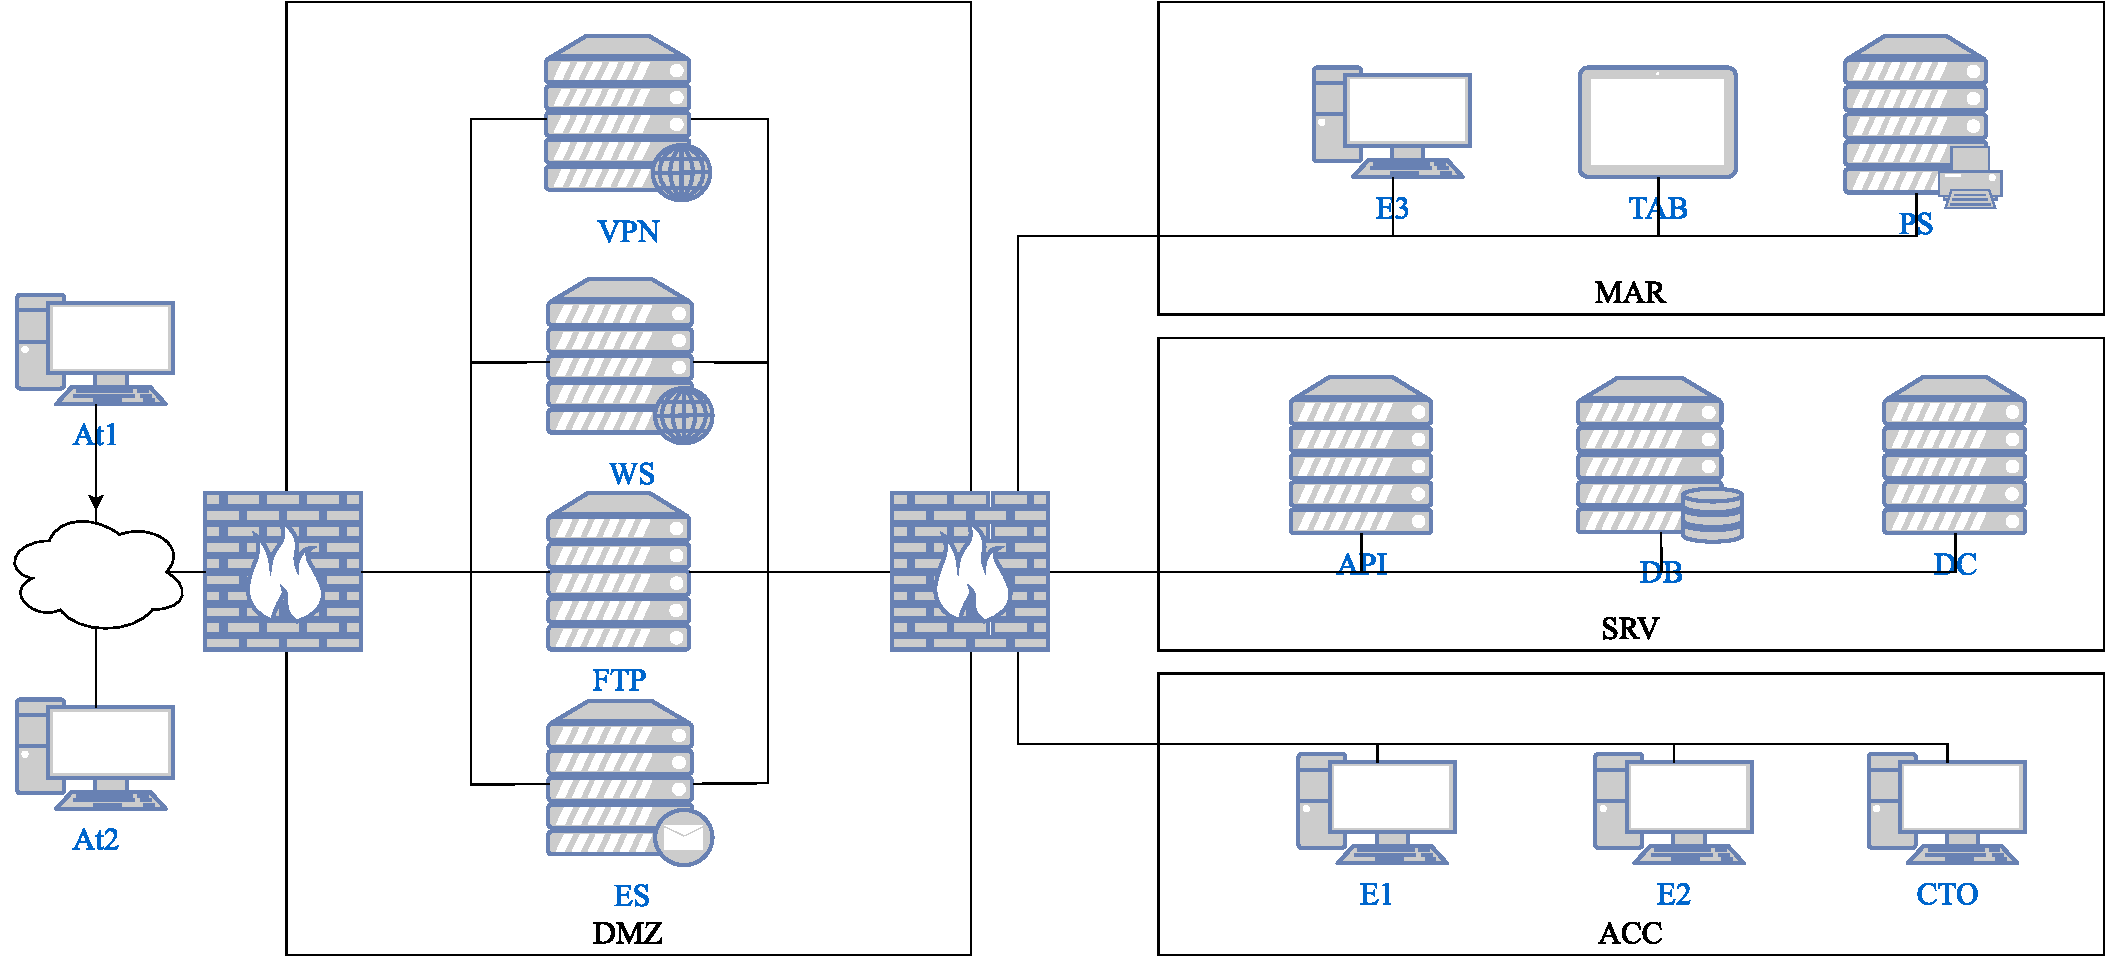
\includegraphics[width=\linewidth]{figures/topology.pdf}
  \caption{Topologie réseau synthétique : EXT (\texttt{At1, At2}), DMZ (\texttt{WS, ES, VPN, FTP}), ACC (\texttt{E1, E2, CTO}), MAR (\texttt{PS, E3, TAB}), SRV (\texttt{API, DB, DC}). Les sous-réseaux sont interconnectés via routeurs/pare-feu implicites.}
  \label{fig:scenario_network_topology}
\end{figure}

\begin{figure}[h!]
  \centering
  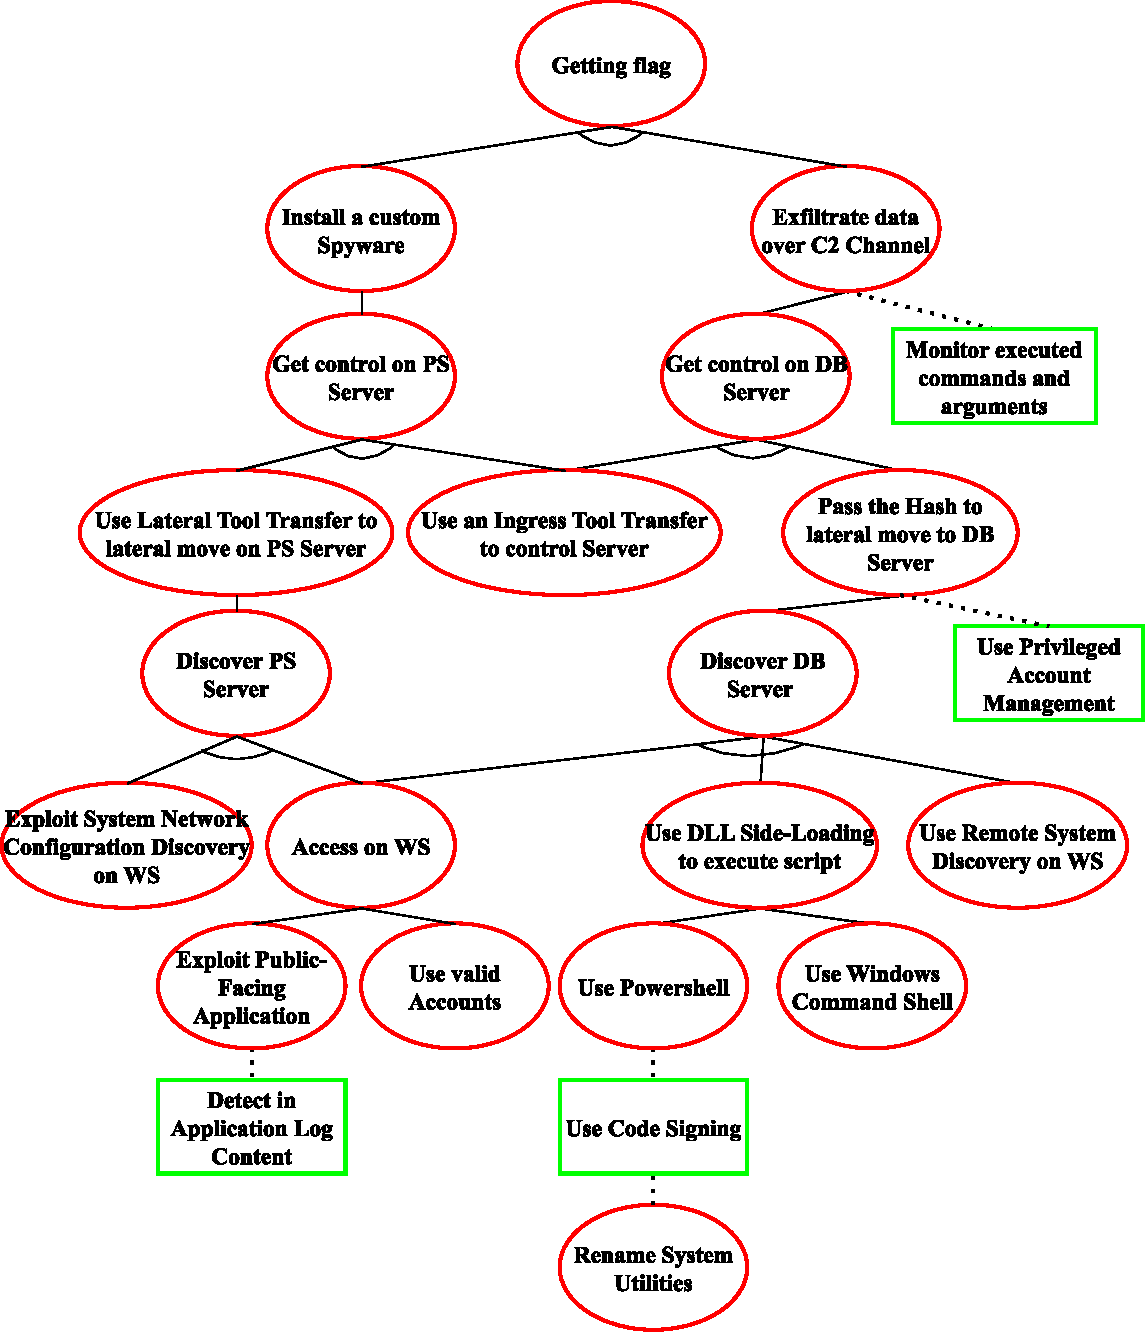
\includegraphics[width=0.86\linewidth]{figures/ADTree.pdf}
  \caption{Aperçu de l’arbre Attaque–Défense (AD) structurant les chemins d’attaque (tactiques/techniques MITRE) et les contre-mesures associées.}
  \label{fig:ADTree}
\end{figure}


\subsection{Description de l'instance du protocole d'experimentation}

\paragraph{1. Configuration initiale}

Nous utilisons le modèle \emph{Dec-POMDP} pré-spécialisé \textbf{Cyberdéfense} et le simulateur \textbf{MCAS} intégrés à \texttt{CybMASDE}, exposés via un adaptateur REST conforme à l’API d’I/O \texttt{CybMASDE} (observations jointes, masques d’actions, \emph{step}/\emph{reset}). L’environnement \emph{Company infrastructure} est donc traité, côté pipeline, exactement comme les environnements jouets non-orientés cyberdéfense : (i) collecte de traces pour la modélisation automatique (\texttt{MOD-AUT}) ; (ii) entraînement MARL (\texttt{TRN}) avec ou sans contraintes organisationnelles ; (iii) analyse organisationnelle (\texttt{ANL}) ; (iv) transfert automatique (\texttt{TRF-AUT}) vers l’exécuteur simulé.
\textbf{Justification :} aucun \texttt{TRF-MAN} n’est requis ici, l’environnement n’étant pas une instrumentation d’un système réel mais un simulateur nativement compatible (pas de « passerelle terrain » à maintenir).
Pour \texttt{MOD-AUT}, un \emph{Joint-Observation Prediction Model} (JOPM : VAE+LSTM) est entraîné sur des historiques mêlant trajectoires aléatoires et politiques préliminaires \emph{rouges/bleues} (progression dans l’AD-tree, détections, quarantaines). Le JOPM approxime la dynamique $\langle o_{1:t},a_{1:t} \rangle \mapsto o_{t+1}$ et fournit une fonction d’arrêt dérivée (objectifs atteints, neutralisation des sessions malveillantes, \emph{step-limit}). La fonction de récompense reconstruite est validée par recoupement avec les métriques natives (progrès le long de l’AD-tree, disponibilité des services). L’entraînement s’appuie sur \texttt{MARLlib}/\texttt{RLlib} (profil \texttt{MAPPO} par défaut, mais variantes testées ci-dessous), \emph{seeds} fixées, 5 exécutions indépendantes comme dans le \autoref{chap:cadre_experimental}. Les conditions de calcul suivent \S\ref{par:compute_conditions} ; seules les dérogations (longueur d’épisode, fréquence de log) sont précisées dans les résultats.

\paragraph{2 à 4. Définition des baselines}

Nous définissons une \textbf{baseline avancée par défaut} et des \textbf{ablations} qui font varier (a) les activités MAMAD (automatisées vs manuelles pour l’analyse), (b) l’algorithme MARL (au moins deux familles), (c) la \emph{dureté} des contraintes organisationnelles : \emph{fortes} (1.0), \emph{douces} (0.5), \emph{sans} (0.0). Toutes reposent sur \texttt{TRF-AUT} (pas de \texttt{TRF-MAN}, cf. justification ci-dessus).

\begin{table*}[h!]
  \centering
  \caption{Baselines synthétiques pour \textbf{Company infrastructure}.}
  \label{tab:baselines_company}
  \renewcommand{\arraystretch}{1}
  \tiny
  \begin{tabularx}{\textwidth}{p{3.8cm}p{2.6cm}p{2.8cm}p{4.6cm}}
    \toprule
    \textbf{Profil d'activités MAMAD} & \textbf{Algorithmes MARL} & \textbf{Contraintes org. (dureté)} & \textbf{Commentaires}                                                                                                                                                          \\
    \midrule
    % --- Profil A (Défaut) ---
    \multirow{3}{*}{\parbox{3.8cm}{\textbf{Profil A — Défaut}                                                                                                                                                                                                                           \\
        \texttt{MOD-AUT};\;\texttt{TRN-CON};\;\texttt{ANL-AUT};\;\texttt{TRF-AUT}}}
                                      & MAPPO, QMIX, COMA         & Oui (1.0)                          & Masquage par rôle (rouge/bleu), shaping aligné AD-tree (progrès d’attaque / détection / quarantaine) ; JOPM activé.                                                            \\
                                      & MAPPO, QMIX, COMA         & Douces (0.5)                       & Même pipeline, pénalités/bonus atténués ; masques partiels (exploration élargie).                                                                                              \\
                                      & MAPPO, QMIX               & Aucune (0.0)                       & \textit{Ablation} TRN-UNC : récompense native (état/metrics), pas de guidage organisationnel.                                                                                  \\
    \midrule
    % --- Profil B (Analyse manuelle) ---
    \multirow{3}{*}{\parbox{3.8cm}{\textbf{Profil B — Analyse manuelle}                                                                                                                                                                                                                 \\
        \texttt{MOD-AUT};\;\texttt{TRN-CON};\;\texttt{ANL-MAN} (TEMM paramétré);\;\texttt{TRF-AUT}}}
                                      & MAPPO, COMA               & Oui (1.0)                          & TEMM (clustering de trajectoires, seuils d’IOC) paramétré à la main ; règles/masques édités (séquencement recon$\rightarrow$exploitation$\rightarrow$LM$\rightarrow$objectif). \\
                                      & MAPPO, COMA               & Douces (0.5)                       & Guidage souple, contrôle post-hoc par TEMM (ajustement seuils de détection, faux positifs).                                                                                    \\
                                      & MAPPO                     & Aucune (0.0)                       & TRN-UNC ; TEMM seulement pour explicabilité/diagnostic (pas de réinjection de règles).                                                                                         \\
    \midrule
    % --- Profil C (Cycle semi-manuel) ---
    \multirow{3}{*}{\parbox{3.8cm}{\textbf{Profil C — Cycle semi-manuel}                                                                                                                                                                                                                \\
        \texttt{MOD-MAN} (actions/props étendues);\;\texttt{TRN-CON} (hp manuels);\;\texttt{ANL-MAN};\;\texttt{TRF-AUT}}}
                                      & IQL, VDN, QMIX            & Oui (1.0)                          & Élargissement « handcrafted » du catalogue d’actions (FW, PAM, persistance) ; hyperparamètres fixés (pas d’HPO).                                                               \\
                                      & IQL, VDN, QMIX            & Douces (0.5)                       & Contraintes souples définies manuellement (seuils journaux/IOC, priorités services).                                                                                           \\
                                      & IQL, VDN                  & Aucune (0.0)                       & Base minimale sans guidage ; utile pour jauger l’apport des contraintes et du shaping.                                                                                         \\
    \bottomrule
  \end{tabularx}
\end{table*}


\section{Description des expérimentations sur l'environnement Microservices Kubernetes}


L'environnement \textbf{Microservices Kubernetes} est un \emph{cluster réel} (1 nœud \textit{worker} : 8 vCPU, 32~Go RAM, 1~Gbps) utilisé comme \emph{environnement d'entrée} de la méthode \acn{MAMAD}. Une illustration schématique de ce cluster et de ses services est fournie en \autoref{fig:k8s_microservices_real}. Le cluster héberge une application web de e-commerce composée de 4 microservices en chaîne (API, Auth, Produits, Commandes) orchestrés via Kubernetes. Chaque service est déployé dans un \emph{pod} avec un nombre variable de réplicas (1 à 5). Le cluster est surveillé en temps réel via Prometheus/Grafana, collectant des métriques telles que l'utilisation CPU/mémoire, le taux de requêtes, la latence, les files d'attente, et l'état des pods. Des scénarios de stress-test sont appliqués pour simuler des conditions réelles : goulots d'étranglement (augmentation du trafic), attaques DDoS (trafic malveillant), pannes de pods (simulées via \texttt{kubectl delete pod}), et contention de ressources (limitation CPU/mémoire). L'objectif est d'évaluer la capacité des agents à maintenir la résilience opérationnelle du cluster en adaptant dynamiquement les ressources et en répondant aux incidents. Une illustration synthétique de ce type de scénarios est fournie en \autoref{fig:k8s_cluster_graph_intro}.

\begin{enumerate*}[label={\roman*)}, itemjoin={;\quad}]
  \item \textbf{Espace d'état :} état courant du cluster réel et des 4 services en chaîne \((i \in \{1..4\})\) :
  \(
  s = \{\text{réplicas}^i,\,
  U_{\text{cpu}}^i, U_{\text{mem}}^i,\,
  T_{\text{in}}^i, T_{\text{out}}^i,\,
  Q_{\text{pending}}^i,\,
  S_{\text{status}}^{i,\text{pods}},\,
  P_{\text{priority}}^i\}_{i=1..4}
  \)
  et agrégats globaux (latence moyenne \(L_{\text{avg}}\), taux de requêtes \(R_{\text{rate}}\), disponibilité)
  \item \textbf{Espace d'observation :} observation \emph{réelle} partielle (Dec-POMDP) obtenue via l’API~Kubernetes/collecte métriques. Elle est \emph{spécifique au rôle} :
  \begin{enumerate*}[label={}, itemjoin={;\,}]
    \item goulots~: \(Q_{\text{pending}}^i, T_{\text{in}}^i/T_{\text{out}}^i\)
    \item DDoS~: \(R_{\text{rate}}, \Delta T, L_{\text{avg}}\)
    \item pannes~: \(S_{\text{status}}^{i,\text{pods}}, F_{\text{fail}}^i\)
    \item ressources~: \(U_{\text{cpu}}^i, U_{\text{mem}}^i, P_{\text{priority}}^i\)
  \end{enumerate*}
  \item \textbf{Espace d'action :} \emph{actions réelles} appliquées au cluster via l’API~Kubernetes :
  \begin{enumerate*}[label={\roman*)}, itemjoin={;\quad}]
    \item \emph{Scaling ciblé} : \texttt{scale\_up}(i), \texttt{scale\_down}(i)
    \item \emph{Gestion DDoS} : \texttt{rate\_limit\_ingress}(i), \texttt{isolate\_service}(i)
    \item \emph{Récupération pannes} : \texttt{restart\_failed\_pod}(i), \texttt{reschedule\_pod}(i)
    \item \emph{Arbitrage ressources} : \texttt{throttle\_low\_prio}(i), \texttt{rebalance\_quota}(i)
  \end{enumerate*}
  \item \textbf{Structure de récompense :} récompense \emph{calculée sur télémétrie réelle} (QoS/résilience) :
  \[
    R_{\text{global}}=
    w_1\cdot\text{SuccessRate}
    -w_2\cdot\overline{Q_{\text{pending}}}
    -w_3\cdot L_{\text{avg}}
    -w_4\cdot \text{DownTime}
    -w_5\cdot \text{OverProvision},
  \]
  complétée par des sous-récompenses par rôle:
  \(R_{\text{bottleneck}}=-\sum_i Q_{\text{pending}}^i\),
  \(R_{\text{ddos}}=-(\text{DownTime}\cdot w_d+L_{\text{avg}}\cdot w_l)\),
  \(R_{\text{failure}}=-\sum_i T_{\text{downtime}}^i\),
  \(R_{\text{resource}}=-\sum_{i\in\text{Critical}}(U_{\text{cpu}}^i+U_{\text{mem}}^i)\)
  \item \textbf{Objectif :} maximiser la \emph{résilience opérationnelle} du cluster réel (taux de réussite élevé, latence/queues faibles, disponibilité maximale) sous 5 scénarios: goulots, DDoS, pannes de pods, contention ressources, \emph{mixte}
\end{enumerate*}

\noindent\textbf{Spécifications organisationnelles :}
\begin{enumerate*}[label={\roman*)}, itemjoin={;\quad}]
  \item \textbf{Rôles :} \texttt{Gestionnaire\_Goulots}, \texttt{Gestionnaire\_DDoS}, \texttt{Gestionnaire\_Pannes}, \texttt{Gestionnaire\_Ressources}
  \item \textbf{Missions :}
  \(\langle\)minimiser \(Q_{\text{pending}}^i\)\(\rangle\);
  \(\langle\)détecter/isoler DDoS et réduire DownTime/latence\(\rangle\);
  \(\langle\)\(\downarrow T_{\text{downtime}}\) par reprise rapide\(\rangle\);
  \(\langle\)prioriser services critiques sous \(U_{\text{cpu/mem}}\) contraint\(\rangle\)
  \item \textbf{Contraintes :}
  (a) \emph{déontiques} par rôle (ex.~seul \texttt{Gestionnaire\_DDoS} peut \texttt{isolate\_service});
  (b) \emph{ségrégation des responsabilités} (éviter des \texttt{scale\_up} contradictoires);
  (c) \emph{garde-fous QoS} (\(Q_{\text{pending}}^i<Q_{\text{seuil}}, U_{\text{cpu}}^{\text{total}}<U_{\text{seuil}}\));
  (d) deux modes d’intégration pendant l’entraînement : \textit{contraintes strictes} (masquage d’actions) vs \textit{souples} (façonnage de récompenses)
\end{enumerate*}

\medskip
\noindent\textit{Remarque (spécificité « réel ») :}
\begin{enumerate*}[label={--}, itemjoin={\quad}]
  \item \textsc{MOD/TRN} sur jumeau numérique dérivé de traces du cluster réel;
  \item \textsc{TRF} : déploiement des politiques apprises sur le cluster via l’API Kubernetes;
  \item sécurité opératoire: actions bornées (quotas/limites), rollbacks et rate-limiting pour préserver la QoS.
\end{enumerate*}

\begin{figure}[h!]
  \centering
  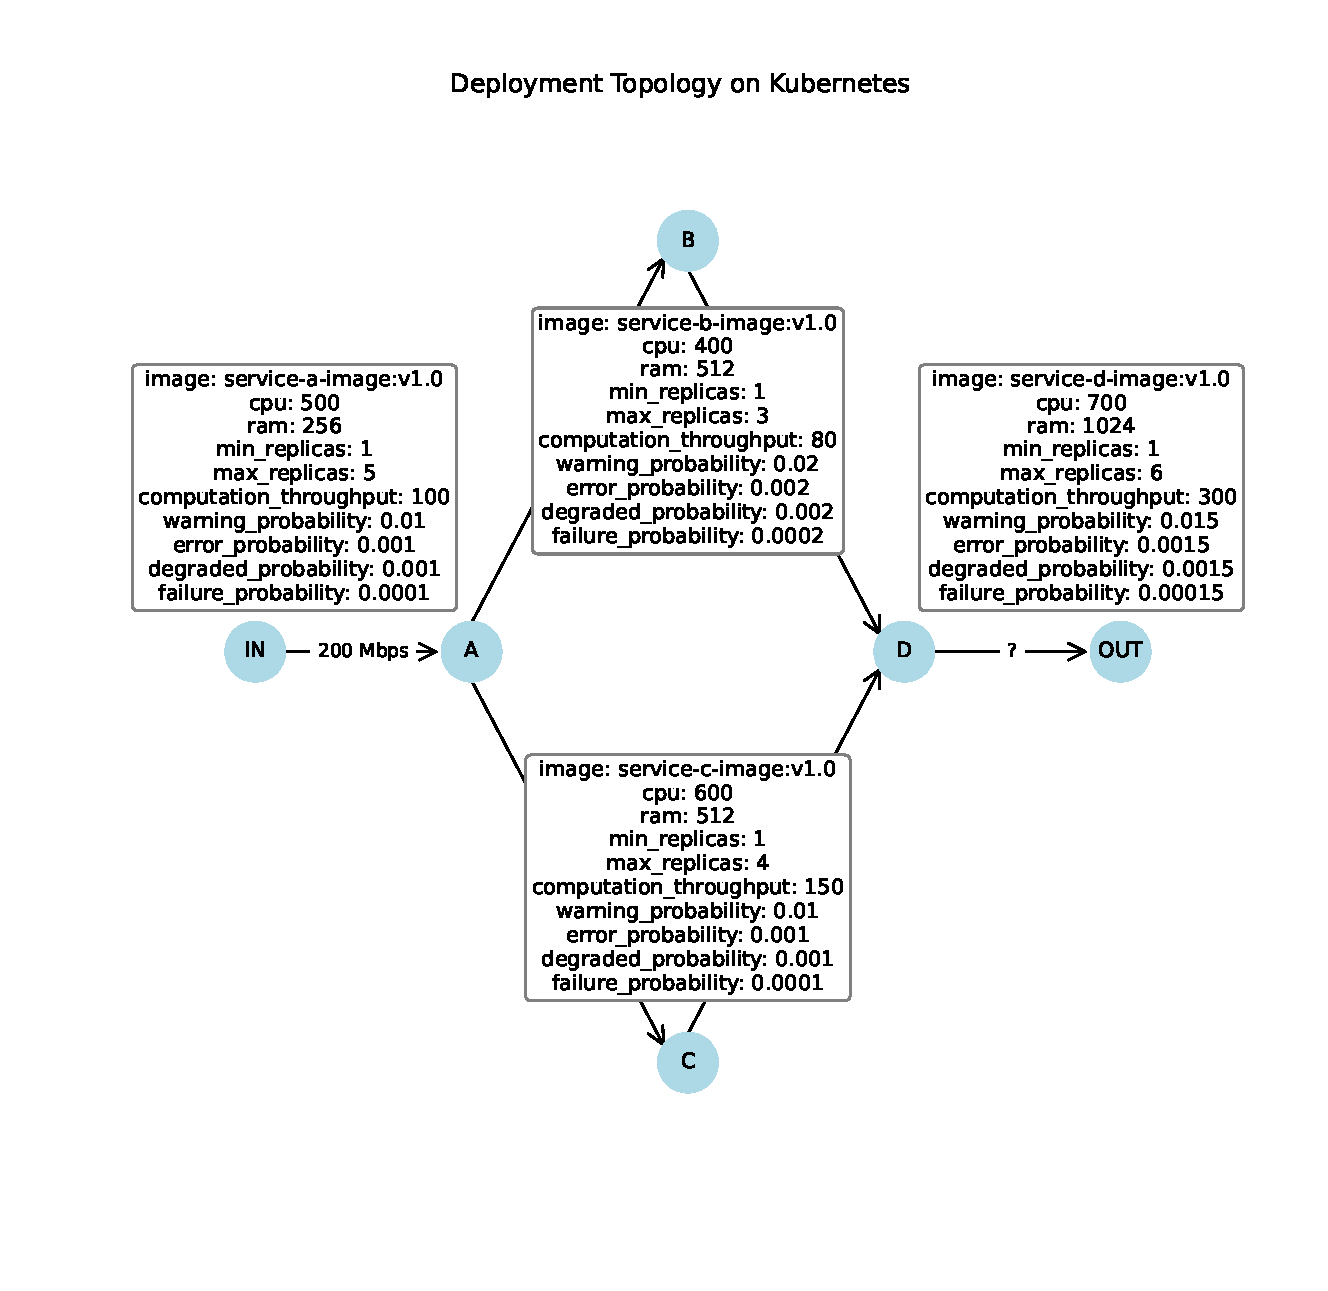
\includegraphics[trim=1.8cm 3.3cm 1.25cm 3.5cm, clip, width=0.6\linewidth]{figures/k8s_cluster_graph.pdf}
  \caption{Cluster \emph{réel} «~Services en chaîne~» (4 services) et leviers d’action exposés à CybMASDE/MAMAD via l’API Kubernetes.}
  \label{fig:k8s_microservices_real}
\end{figure}

\begin{figure}[h!]
  \centering
  \hspace{-0.4cm}
  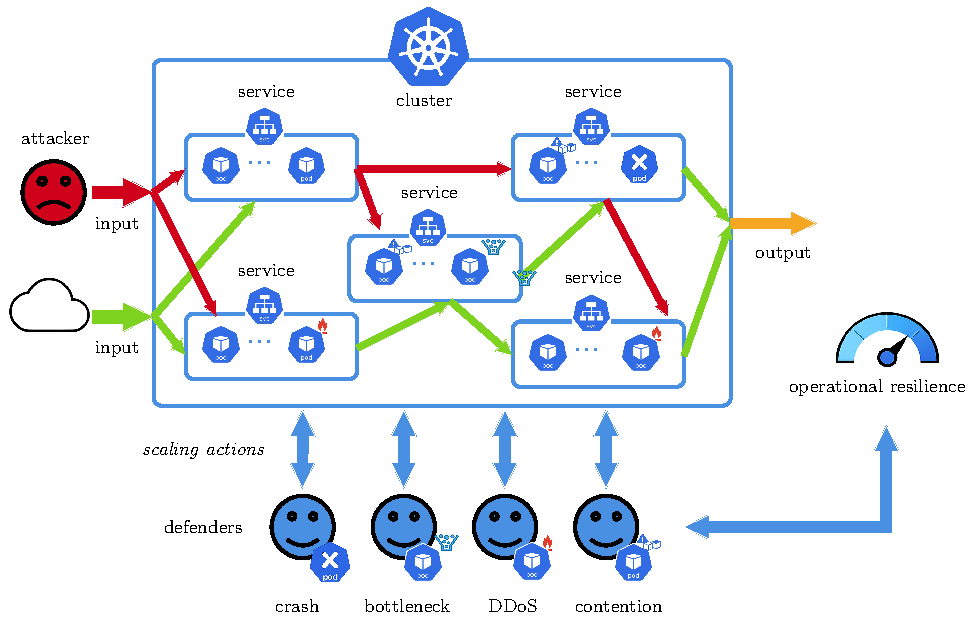
\includegraphics[trim=0cm 0cm 0cm 0cm, clip, width=0.5\textwidth]{figures/scenario_introduction.pdf}
  \caption{Une vue abstraite du scénario de cluster Kubernetes où chaque service s’exécute en pods gérés par des \textit{Deployments} et peut être répliqué dynamiquement. Des agents défenseurs ayant des rôles spécifiques (p.,ex. \textit{détecteur DDoS}, \textit{gestionnaire de ressources}, \textit{gestionnaire de goulots}, \textit{gestionnaire de pannes}) observent en continu les métriques clés (latence, requêtes en attente, trafic entrant/sortant, états des pods, utilisation CPU/mémoire) et appliquent via l’API Kubernetes des \textit{scaling actions} (mode \textit{REMOTE}) pour ajuster les réplicas, isoler des services affectés ou relancer des composants défaillants. L’illustration met en évidence quatre familles de perturbations ciblant la chaîne — \textit{bottleneck} (engorgement), \textit{contention} (conflit de ressources), \textit{crash} (défaillance de pods) et \textit{DDoS}/injections massives — ainsi que des compromissions de pods ; les agents doivent détecter les anomalies, isoler/segmenter les composants compromis et réallouer les ressources pour préserver la \textit{résilience opérationnelle} globale (disponibilité, débit, latence) et minimiser l’impact pour les utilisateurs finaux.}
  \label{fig:k8s_cluster_graph_intro}
\end{figure}


\subsection{Description de l'instance du protocole d'expérimentation}

\paragraph{1. Configuration initiale}

Nous opérons \emph{sur le cluster réel} (pas de simulation en ligne de commande jouant le rôle d’« environnement réel »). Le cluster (\textbf{VM 8~vCPU, 32~Go RAM, 1~Gbps}) héberge l’application e-commerce (4 microservices en chaîne). La télémétrie est collectée par \textit{Prometheus} et visualisée via \textit{Grafana}. \texttt{CybMASDE}/\texttt{KARMA} s’interface avec l’API Kubernetes pour \textit{observer} l’état et \textit{agir} (scaling, isolement, redémarrage). Un \textbf{jumeau numérique} est construit à partir des traces pour entraîner les politiques hors-ligne puis \textbf{transférées} et \textit{fermées en boucle} sur le cluster (apprentissage itératif par rafraîchissement des traces).

\begin{figure}[h!]
  \centering
  


\tikzset{every picture/.style={line width=0.75pt}} %set default line width to 0.75pt        

\begin{tikzpicture}[x=0.75pt,y=0.75pt,yscale=-1.2,xscale=1.2]
%uncomment if require: \path (0,1414); %set diagram left start at 0, and has height of 1414

%Straight Lines [id:da5609883377896374] 
\draw [color={rgb, 255:red, 74; green, 144; blue, 226 }  ,draw opacity=1 ][line width=2.25]    (317.22,111.13) -- (360.07,111.13) ;
\draw [shift={(365.07,111.13)}, rotate = 180] [fill={rgb, 255:red, 74; green, 144; blue, 226 }  ,fill opacity=1 ][line width=0.08]  [draw opacity=0] (5.72,-2.75) -- (0,0) -- (5.72,2.75) -- cycle    ;
%Image [id:dp9396292457736715] 
\draw (106.77,60.95) node  {
\includegraphics[width=18.66pt,height=18.36pt]{figures/karma_architecture/pod.png}};
%Image [id:dp3874378335758297] 
\draw (145.86,60.95) node  {
\includegraphics[width=18.66pt,height=18.36pt]{figures/karma_architecture/pod.png}};
%Shape: Rectangle [id:dp4562827234223257] 
\draw  [color={rgb, 255:red, 74; green, 144; blue, 226 }  ,draw opacity=1 ][line width=1.5]  (89,28.36) .. controls (89,25.6) and (91.24,23.36) .. (94,23.36) -- (255,23.36) .. controls (257.76,23.36) and (260,25.6) .. (260,28.36) -- (260,132) .. controls (260,134.76) and (257.76,137) .. (255,137) -- (94,137) .. controls (91.24,137) and (89,134.76) .. (89,132) -- cycle ;
%Image [id:dp9455935833751838] 
\draw (172.5,16.24) node  {
\includegraphics[width=18.66pt,height=18.36pt]{figures/karma_architecture/kubernetes.png}};
%Shape: Rectangle [id:dp9564725691593288] 
\draw  [color={rgb, 255:red, 74; green, 144; blue, 226 }  ,draw opacity=1 ][line width=1.5]  (92.55,50.21) .. controls (92.55,47.45) and (94.79,45.21) .. (97.55,45.21) -- (155.08,45.21) .. controls (157.84,45.21) and (160.08,47.45) .. (160.08,50.21) -- (160.08,70.81) .. controls (160.08,73.57) and (157.84,75.81) .. (155.08,75.81) -- (97.55,75.81) .. controls (94.79,75.81) and (92.55,73.57) .. (92.55,70.81) -- cycle ;
%Image [id:dp9120856447688912] 
\draw (126.32,39.97) node  {
\includegraphics[width=18.66pt,height=18.36pt]{figures/karma_architecture/node.png}};
%Image [id:dp5738167237736518] 
\draw (106.77,119.52) node  {
\includegraphics[width=18.66pt,height=18.36pt]{figures/karma_architecture/pod.png}};
%Image [id:dp2199681121060142] 
\draw (145.86,119.52) node  {
\includegraphics[width=18.66pt,height=18.36pt]{figures/karma_architecture/pod.png}};
%Shape: Rectangle [id:dp12159705904547402] 
\draw  [color={rgb, 255:red, 74; green, 144; blue, 226 }  ,draw opacity=1 ][line width=1.5]  (92.55,108.78) .. controls (92.55,106.02) and (94.79,103.78) .. (97.55,103.78) -- (155.08,103.78) .. controls (157.84,103.78) and (160.08,106.02) .. (160.08,108.78) -- (160.08,129.38) .. controls (160.08,132.14) and (157.84,134.38) .. (155.08,134.38) -- (97.55,134.38) .. controls (94.79,134.38) and (92.55,132.14) .. (92.55,129.38) -- cycle ;
%Image [id:dp37768653229718074] 
\draw (126.32,98.54) node  {
\includegraphics[width=18.66pt,height=18.36pt]{figures/karma_architecture/node.png}};
%Shape: Rectangle [id:dp20840815212238661] 
\draw  [color={rgb, 255:red, 74; green, 144; blue, 226 }  ,draw opacity=1 ][line width=1.5]  (264,28.36) .. controls (264,25.6) and (266.24,23.36) .. (269,23.36) -- (411.78,23.36) .. controls (414.54,23.36) and (416.78,25.6) .. (416.78,28.36) -- (416.78,132) .. controls (416.78,134.76) and (414.54,137) .. (411.78,137) -- (269,137) .. controls (266.24,137) and (264,134.76) .. (264,132) -- cycle ;
%Straight Lines [id:da9232180983272227] 
\draw [color={rgb, 255:red, 74; green, 144; blue, 226 }  ,draw opacity=1 ][line width=2.25]    (164,112) -- (201,112) ;
\draw [shift={(206,112)}, rotate = 180] [fill={rgb, 255:red, 74; green, 144; blue, 226 }  ,fill opacity=1 ][line width=0.08]  [draw opacity=0] (5.72,-2.75) -- (0,0) -- (5.72,2.75) -- cycle    ;
%Straight Lines [id:da6082715106712999] 
\draw [color={rgb, 255:red, 74; green, 144; blue, 226 }  ,draw opacity=1 ][line width=2.25]    (180,90.22) -- (167,90.22) ;
\draw [shift={(162,90.22)}, rotate = 360] [fill={rgb, 255:red, 74; green, 144; blue, 226 }  ,fill opacity=1 ][line width=0.08]  [draw opacity=0] (5.72,-2.75) -- (0,0) -- (5.72,2.75) -- cycle    ;
%Straight Lines [id:da30764510910060716] 
\draw [color={rgb, 255:red, 74; green, 144; blue, 226 }  ,draw opacity=1 ][line width=2.25]    (210,72) -- (199,72) ;
\draw [shift={(194,72)}, rotate = 360] [fill={rgb, 255:red, 74; green, 144; blue, 226 }  ,fill opacity=1 ][line width=0.08]  [draw opacity=0] (5.72,-2.75) -- (0,0) -- (5.72,2.75) -- cycle    ;
%Straight Lines [id:da5394403186779959] 
\draw [color={rgb, 255:red, 74; green, 144; blue, 226 }  ,draw opacity=1 ][line width=2.25]    (178,56.22) -- (167,56.22) ;
\draw [shift={(162,56.22)}, rotate = 360] [fill={rgb, 255:red, 74; green, 144; blue, 226 }  ,fill opacity=1 ][line width=0.08]  [draw opacity=0] (5.72,-2.75) -- (0,0) -- (5.72,2.75) -- cycle    ;
%Straight Lines [id:da6399475815904785] 
\draw [color={rgb, 255:red, 74; green, 144; blue, 226 }  ,draw opacity=1 ][line width=2.25]    (272,72) -- (235,72) ;
\draw [shift={(230,72)}, rotate = 360] [fill={rgb, 255:red, 74; green, 144; blue, 226 }  ,fill opacity=1 ][line width=0.08]  [draw opacity=0] (5.72,-2.75) -- (0,0) -- (5.72,2.75) -- cycle    ;
%Straight Lines [id:da24320102833940327] 
\draw [color={rgb, 255:red, 74; green, 144; blue, 226 }  ,draw opacity=1 ][line width=2.25]    (267,112) -- (230,112) ;
\draw [shift={(272,112)}, rotate = 180] [fill={rgb, 255:red, 74; green, 144; blue, 226 }  ,fill opacity=1 ][line width=0.08]  [draw opacity=0] (5.72,-2.75) -- (0,0) -- (5.72,2.75) -- cycle    ;
%Shape: Rectangle [id:dp9149123987409296] 
\draw  [color={rgb, 255:red, 255; green, 255; blue, 255 }  ,draw opacity=1 ][fill={rgb, 255:red, 255; green, 255; blue, 255 }  ,fill opacity=1 ] (328.83,106.67) -- (353.11,106.67) -- (353.11,114) -- (328.83,114) -- cycle ;
%Image [id:dp7127891043436136] 
\draw (341.68,109.47) node  {
\includegraphics[width=14.57pt,height=15.21pt]{figures/karma_architecture/pettingzoo.png}};
%Straight Lines [id:da5757027637146572] 
\draw [color={rgb, 255:red, 74; green, 144; blue, 226 }  ,draw opacity=1 ][line width=2.25]    (357.9,41) -- (364.9,41) ;
\draw [shift={(352.9,41)}, rotate = 0] [fill={rgb, 255:red, 74; green, 144; blue, 226 }  ,fill opacity=1 ][line width=0.08]  [draw opacity=0] (5.72,-2.75) -- (0,0) -- (5.72,2.75) -- cycle    ;
%Straight Lines [id:da29364722138505184] 
\draw [color={rgb, 255:red, 74; green, 144; blue, 226 }  ,draw opacity=1 ][line width=2.25]    (390.99,97.77) -- (390.99,57.25) ;
\draw [shift={(390.99,52.25)}, rotate = 90] [fill={rgb, 255:red, 74; green, 144; blue, 226 }  ,fill opacity=1 ][line width=0.08]  [draw opacity=0] (5.72,-2.75) -- (0,0) -- (5.72,2.75) -- cycle    ;
%Straight Lines [id:da5470457469462804] 
\draw [color={rgb, 255:red, 74; green, 144; blue, 226 }  ,draw opacity=1 ][line width=2.25]    (390.9,71) -- (325.9,71) ;
\draw [shift={(320.9,71)}, rotate = 360] [fill={rgb, 255:red, 74; green, 144; blue, 226 }  ,fill opacity=1 ][line width=0.08]  [draw opacity=0] (5.72,-2.75) -- (0,0) -- (5.72,2.75) -- cycle    ;
%Shape: Rectangle [id:dp8476965567779329] 
\draw  [color={rgb, 255:red, 255; green, 255; blue, 255 }  ,draw opacity=1 ][fill={rgb, 255:red, 255; green, 255; blue, 255 }  ,fill opacity=1 ] (378.41,65.11) -- (397.83,65.11) -- (397.83,92) -- (378.41,92) -- cycle ;
%Shape: Smiley Face [id:dp8656850497140396] 
\draw  [fill={rgb, 255:red, 255; green, 255; blue, 255 }  ,fill opacity=1 ][line width=0.75]  (380.35,69.4) .. controls (380.35,67.3) and (382.09,65.6) .. (384.24,65.6) .. controls (386.38,65.6) and (388.12,67.3) .. (388.12,69.4) .. controls (388.12,71.5) and (386.38,73.2) .. (384.24,73.2) .. controls (382.09,73.2) and (380.35,71.5) .. (380.35,69.4) -- cycle ; \draw  [fill={rgb, 255:red, 255; green, 255; blue, 255 }  ,fill opacity=1 ][line width=0.75]  (382.53,68.11) .. controls (382.53,67.9) and (382.7,67.73) .. (382.92,67.73) .. controls (383.13,67.73) and (383.31,67.9) .. (383.31,68.11) .. controls (383.31,68.32) and (383.13,68.49) .. (382.92,68.49) .. controls (382.7,68.49) and (382.53,68.32) .. (382.53,68.11) -- cycle ; \draw  [fill={rgb, 255:red, 255; green, 255; blue, 255 }  ,fill opacity=1 ][line width=0.75]  (385.17,68.11) .. controls (385.17,67.9) and (385.34,67.73) .. (385.56,67.73) .. controls (385.77,67.73) and (385.95,67.9) .. (385.95,68.11) .. controls (385.95,68.32) and (385.77,68.49) .. (385.56,68.49) .. controls (385.34,68.49) and (385.17,68.32) .. (385.17,68.11) -- cycle ; \draw  [line width=0.75]  (382.29,70.92) .. controls (383.59,71.94) and (384.88,71.94) .. (386.18,70.92) ;
%Shape: Smiley Face [id:dp9163740789669144] 
\draw  [fill={rgb, 255:red, 255; green, 255; blue, 255 }  ,fill opacity=1 ][line width=0.75]  (392.01,69.4) .. controls (392.01,67.3) and (393.75,65.6) .. (395.89,65.6) .. controls (398.04,65.6) and (399.78,67.3) .. (399.78,69.4) .. controls (399.78,71.5) and (398.04,73.2) .. (395.89,73.2) .. controls (393.75,73.2) and (392.01,71.5) .. (392.01,69.4) -- cycle ; \draw  [fill={rgb, 255:red, 255; green, 255; blue, 255 }  ,fill opacity=1 ][line width=0.75]  (394.18,68.11) .. controls (394.18,67.9) and (394.36,67.73) .. (394.57,67.73) .. controls (394.79,67.73) and (394.96,67.9) .. (394.96,68.11) .. controls (394.96,68.32) and (394.79,68.49) .. (394.57,68.49) .. controls (394.36,68.49) and (394.18,68.32) .. (394.18,68.11) -- cycle ; \draw  [fill={rgb, 255:red, 255; green, 255; blue, 255 }  ,fill opacity=1 ][line width=0.75]  (396.82,68.11) .. controls (396.82,67.9) and (397,67.73) .. (397.21,67.73) .. controls (397.43,67.73) and (397.6,67.9) .. (397.6,68.11) .. controls (397.6,68.32) and (397.43,68.49) .. (397.21,68.49) .. controls (397,68.49) and (396.82,68.32) .. (396.82,68.11) -- cycle ; \draw  [line width=0.75]  (393.95,70.92) .. controls (395.24,71.94) and (396.54,71.94) .. (397.83,70.92) ;
%Shape: Smiley Face [id:dp8186451078369623] 
\draw  [fill={rgb, 255:red, 255; green, 255; blue, 255 }  ,fill opacity=1 ][line width=0.75]  (386.18,77.44) .. controls (386.18,75.34) and (387.92,73.64) .. (390.06,73.64) .. controls (392.21,73.64) and (393.95,75.34) .. (393.95,77.44) .. controls (393.95,79.54) and (392.21,81.24) .. (390.06,81.24) .. controls (387.92,81.24) and (386.18,79.54) .. (386.18,77.44) -- cycle ; \draw  [fill={rgb, 255:red, 255; green, 255; blue, 255 }  ,fill opacity=1 ][line width=0.75]  (388.36,76.15) .. controls (388.36,75.94) and (388.53,75.77) .. (388.74,75.77) .. controls (388.96,75.77) and (389.13,75.94) .. (389.13,76.15) .. controls (389.13,76.36) and (388.96,76.53) .. (388.74,76.53) .. controls (388.53,76.53) and (388.36,76.36) .. (388.36,76.15) -- cycle ; \draw  [fill={rgb, 255:red, 255; green, 255; blue, 255 }  ,fill opacity=1 ][line width=0.75]  (391,76.15) .. controls (391,75.94) and (391.17,75.77) .. (391.39,75.77) .. controls (391.6,75.77) and (391.77,75.94) .. (391.77,76.15) .. controls (391.77,76.36) and (391.6,76.53) .. (391.39,76.53) .. controls (391.17,76.53) and (391,76.36) .. (391,76.15) -- cycle ; \draw  [line width=0.75]  (388.12,78.96) .. controls (389.42,79.98) and (390.71,79.98) .. (392.01,78.96) ;
%Flowchart: Punched Tape [id:dp6020643269389074] 
\draw  [fill={rgb, 255:red, 255; green, 255; blue, 255 }  ,fill opacity=1 ] (313.9,33.81) .. controls (313.9,35.03) and (318.18,36.02) .. (323.45,36.02) .. controls (328.73,36.02) and (333,35.03) .. (333,33.81) .. controls (333,32.58) and (337.28,31.59) .. (342.55,31.59) .. controls (347.83,31.59) and (352.1,32.58) .. (352.1,33.81) -- (352.1,51.52) .. controls (352.1,50.3) and (347.83,49.31) .. (342.55,49.31) .. controls (337.28,49.31) and (333,50.3) .. (333,51.52) .. controls (333,52.75) and (328.73,53.74) .. (323.45,53.74) .. controls (318.18,53.74) and (313.9,52.75) .. (313.9,51.52) -- cycle ;
%Straight Lines [id:da950307097731951] 
\draw [line width=0.75]    (324.14,41.04) -- (341.9,41) ;
%Shape: Smiley Face [id:dp8914579811118104] 
\draw  [line width=0.75]  (320.58,40.88) .. controls (320.58,39.7) and (321.59,38.73) .. (322.85,38.73) .. controls (324.1,38.73) and (325.11,39.7) .. (325.11,40.88) .. controls (325.11,42.07) and (324.1,43.03) .. (322.85,43.03) .. controls (321.59,43.03) and (320.58,42.07) .. (320.58,40.88) -- cycle ; \draw  [line width=0.75]  (321.85,40.15) .. controls (321.85,40.03) and (321.95,39.94) .. (322.08,39.94) .. controls (322.2,39.94) and (322.3,40.03) .. (322.3,40.15) .. controls (322.3,40.27) and (322.2,40.37) .. (322.08,40.37) .. controls (321.95,40.37) and (321.85,40.27) .. (321.85,40.15) -- cycle ; \draw  [line width=0.75]  (323.39,40.15) .. controls (323.39,40.03) and (323.49,39.94) .. (323.62,39.94) .. controls (323.74,39.94) and (323.84,40.03) .. (323.84,40.15) .. controls (323.84,40.27) and (323.74,40.37) .. (323.62,40.37) .. controls (323.49,40.37) and (323.39,40.27) .. (323.39,40.15) -- cycle ; \draw  [line width=0.75]  (321.71,41.74) .. controls (322.47,42.31) and (323.22,42.31) .. (323.98,41.74) ;
%Shape: Smiley Face [id:dp07941198495535606] 
\draw  [line width=0.75]  (329.9,45.15) .. controls (329.9,43.96) and (330.92,43) .. (332.17,43) .. controls (333.42,43) and (334.44,43.96) .. (334.44,45.15) .. controls (334.44,46.33) and (333.42,47.29) .. (332.17,47.29) .. controls (330.92,47.29) and (329.9,46.33) .. (329.9,45.15) -- cycle ; \draw  [line width=0.75]  (331.17,44.42) .. controls (331.17,44.3) and (331.28,44.2) .. (331.4,44.2) .. controls (331.53,44.2) and (331.63,44.3) .. (331.63,44.42) .. controls (331.63,44.54) and (331.53,44.63) .. (331.4,44.63) .. controls (331.28,44.63) and (331.17,44.54) .. (331.17,44.42) -- cycle ; \draw  [line width=0.75]  (332.72,44.42) .. controls (332.72,44.3) and (332.82,44.2) .. (332.94,44.2) .. controls (333.07,44.2) and (333.17,44.3) .. (333.17,44.42) .. controls (333.17,44.54) and (333.07,44.63) .. (332.94,44.63) .. controls (332.82,44.63) and (332.72,44.54) .. (332.72,44.42) -- cycle ; \draw  [line width=0.75]  (331.04,46.01) .. controls (331.79,46.58) and (332.55,46.58) .. (333.3,46.01) ;
%Shape: Smiley Face [id:dp8353415903298282] 
\draw  [line width=0.75]  (341.9,40.85) .. controls (341.9,39.67) and (342.92,38.71) .. (344.17,38.71) .. controls (345.42,38.71) and (346.44,39.67) .. (346.44,40.85) .. controls (346.44,42.04) and (345.42,43) .. (344.17,43) .. controls (342.92,43) and (341.9,42.04) .. (341.9,40.85) -- cycle ; \draw  [line width=0.75]  (343.17,40.12) .. controls (343.17,40) and (343.28,39.91) .. (343.4,39.91) .. controls (343.53,39.91) and (343.63,40) .. (343.63,40.12) .. controls (343.63,40.24) and (343.53,40.34) .. (343.4,40.34) .. controls (343.28,40.34) and (343.17,40.24) .. (343.17,40.12) -- cycle ; \draw  [line width=0.75]  (344.72,40.12) .. controls (344.72,40) and (344.82,39.91) .. (344.94,39.91) .. controls (345.07,39.91) and (345.17,40) .. (345.17,40.12) .. controls (345.17,40.24) and (345.07,40.34) .. (344.94,40.34) .. controls (344.82,40.34) and (344.72,40.24) .. (344.72,40.12) -- cycle ; \draw  [line width=0.75]  (343.04,41.71) .. controls (343.79,42.28) and (344.55,42.28) .. (345.3,41.71) ;
%Straight Lines [id:da21936285199788075] 
\draw [line width=0.75]    (324.19,41.87) -- (329.9,45) ;
%Image [id:dp05694376090002984] 
\draw (218.44,70.24) node  {
\includegraphics[width=18.66pt,height=18.36pt]{figures/karma_architecture/api.png}};
%Image [id:dp7747210194064744] 
\draw (186.74,54.54) node  {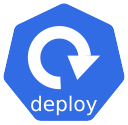
\includegraphics[width=18.66pt,height=18.36pt]{figures/karma_architecture/deploy.png}};
%Image [id:dp5268588430037433] 
\draw (186.74,87.76) node  {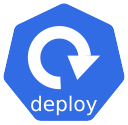
\includegraphics[width=18.66pt,height=18.36pt]{figures/karma_architecture/deploy.png}};
%Image [id:dp7447308292951857] 
\draw (218.44,111.76) node  {
\includegraphics[width=18.66pt,height=18.36pt]{figures/karma_architecture/prometheus.png}};
%Shape: Rectangle [id:dp7837974954754439] 
\draw  [color={rgb, 255:red, 75; green, 101; blue, 225 }  ,draw opacity=1 ][fill={rgb, 255:red, 74; green, 144; blue, 226 }  ,fill opacity=1 ] (202.37,94.64) -- (208.29,94.64) -- (208.29,101.67) -- (202.37,101.67) -- cycle ;
%Shape: Rectangle [id:dp780870970882084] 
\draw  [color={rgb, 255:red, 75; green, 101; blue, 225 }  ,draw opacity=1 ][fill={rgb, 255:red, 74; green, 144; blue, 226 }  ,fill opacity=1 ] (286.37,126) -- (292.29,126) -- (292.29,133.03) -- (286.37,133.03) -- cycle ;

%Shape: Rectangle [id:dp7051683429553395] 
\draw  [color={rgb, 255:red, 75; green, 101; blue, 225 }  ,draw opacity=1 ][fill={rgb, 255:red, 74; green, 144; blue, 226 }  ,fill opacity=1 ] (397.37,124.64) -- (403.29,124.64) -- (403.29,131.67) -- (397.37,131.67) -- cycle ;

%Shape: Rectangle [id:dp5578959475333973] 
\draw  [color={rgb, 255:red, 75; green, 101; blue, 225 }  ,draw opacity=1 ][fill={rgb, 255:red, 74; green, 144; blue, 226 }  ,fill opacity=1 ] (368.37,54.64) -- (374.29,54.64) -- (374.29,61.67) -- (368.37,61.67) -- cycle ;

%Shape: Rectangle [id:dp2822949836407178] 
\draw  [color={rgb, 255:red, 75; green, 101; blue, 225 }  ,draw opacity=1 ][fill={rgb, 255:red, 74; green, 144; blue, 226 }  ,fill opacity=1 ] (324.37,78) -- (330.29,78) -- (330.29,85.03) -- (324.37,85.03) -- cycle ;

%Shape: Rectangle [id:dp9339299822588341] 
\draw  [color={rgb, 255:red, 75; green, 101; blue, 225 }  ,draw opacity=1 ][fill={rgb, 255:red, 74; green, 144; blue, 226 }  ,fill opacity=1 ] (205.37,48) -- (211.29,48) -- (211.29,55.03) -- (205.37,55.03) -- cycle ;



% Text Node
\draw (205.5,98.5) node  [font=\fontsize{0.33em}{0.4em}\selectfont,color={rgb, 255:red, 255; green, 255; blue, 255 }  ,opacity=1 ] [align=left] {1};
% Text Node
\draw (244,58.5) node  [font=\normalsize] [align=left] {{\tiny Scaling}};
\draw (244,64.5) node  [font=\normalsize] [align=left] {{\tiny actions}};
% Text Node
\draw (244,99.5) node  [font=\normalsize] [align=left] {{\tiny Metrics}};
\draw (244,105.5) node  [font=\normalsize] [align=left] {{\tiny data}};
% Text Node
\draw (344.5,36) node  [font=\fontsize{0.33em}{0.4em}\selectfont] [align=left] {\begin{minipage}[lt]{8.66pt}\setlength\topsep{0pt}
\begin{center}
{\fontsize{0.33em}{0.4em}\selectfont $\displaystyle \mathbf{\textcolor[rgb]{0.82,0.01,0.11}{\pi }\textcolor[rgb]{0.82,0.01,0.11}{_{3}}}$}
\end{center}

\end{minipage}};
% Text Node
\draw (341,46.5) node  [font=\fontsize{0.33em}{0.4em}\selectfont] [align=left] {\begin{minipage}[lt]{8.66pt}\setlength\topsep{0pt}
\begin{center}
{\fontsize{0.33em}{0.4em}\selectfont $\displaystyle \mathbf{\textcolor[rgb]{0.82,0.01,0.11}{\pi }\textcolor[rgb]{0.82,0.01,0.11}{_{2}}}$}
\end{center}

\end{minipage}};
% Text Node
\draw (320.9,48) node  [font=\fontsize{0.33em}{0.4em}\selectfont] [align=left] {\begin{minipage}[lt]{8.66pt}\setlength\topsep{0pt}
\begin{center}
{\fontsize{0.33em}{0.4em}\selectfont $\displaystyle \mathbf{\textcolor[rgb]{0.82,0.01,0.11}{\pi }\textcolor[rgb]{0.82,0.01,0.11}{_{1}}}$}
\end{center}

\end{minipage}};
% Text Node
\draw  [color={rgb, 255:red, 75; green, 101; blue, 225 }  ,draw opacity=1 ][fill={rgb, 255:red, 136; green, 197; blue, 246 }  ,fill opacity=1 ][line width=1.5]   (322.77,14.89) .. controls (322.77,13.78) and (323.67,12.89) .. (324.77,12.89) -- (355.77,12.89) .. controls (356.88,12.89) and (357.77,13.78) .. (357.77,14.89) -- (357.77,26.89) .. controls (357.77,27.99) and (356.88,28.89) .. (355.77,28.89) -- (324.77,28.89) .. controls (323.67,28.89) and (322.77,27.99) .. (322.77,26.89) -- cycle  ;
\draw (340.27,20.89) node  [font=\tiny] [align=left] {\begin{minipage}[lt]{21.5pt}\setlength\topsep{0pt}
\begin{center}
KARMA
\end{center}

\end{minipage}};
% Text Node
\draw (290,40.5) node  [font=\tiny] [align=left] {\begin{minipage}[lt]{27.24pt}\setlength\topsep{0pt}
\begin{center}
Organizational\\Analysis
\end{center}

\end{minipage}};
% Text Node
\draw (388,86.39) node  [font=\tiny] [align=left] {\begin{minipage}[lt]{43.42pt}\setlength\topsep{0pt}
\begin{center}
Trained policies
\end{center}

\end{minipage}};
% Text Node
\draw (344.13,127.35) node  [font=\tiny] [align=left] {\begin{minipage}[lt]{60.78pt}\setlength\topsep{0pt}
\begin{center}
PettingZoo environment
\end{center}

\end{minipage}};
% Text Node
\draw (218,127) node  [font=\tiny] [align=left] {\begin{minipage}[lt]{30.31pt}\setlength\topsep{0pt}
\begin{center}
Prometheus
\end{center}

\end{minipage}};
% Text Node
\draw  [color={rgb, 255:red, 75; green, 101; blue, 225 }  ,draw opacity=1 ][fill={rgb, 255:red, 136; green, 197; blue, 246 }  ,fill opacity=1 ][line width=1.5]   (272.9,62) .. controls (272.9,60.9) and (273.8,60) .. (274.9,60) -- (317.9,60) .. controls (319.01,60) and (319.9,60.9) .. (319.9,62) -- (319.9,83) .. controls (319.9,84.1) and (319.01,85) .. (317.9,85) -- (274.9,85) .. controls (273.8,85) and (272.9,84.1) .. (272.9,83) -- cycle  ;
\draw (296.4,72.5) node  [font=\tiny,color={rgb, 255:red, 0; green, 0; blue, 0 }  ,opacity=1 ] [align=left] {Transfer\\Component};
% Text Node
\draw  [color={rgb, 255:red, 75; green, 101; blue, 225 }  ,draw opacity=1 ][fill={rgb, 255:red, 136; green, 197; blue, 246 }  ,fill opacity=1 ][line width=1.5]   (365.88,29.46) .. controls (365.88,28.35) and (366.78,27.46) .. (367.88,27.46) -- (410.88,27.46) .. controls (411.99,27.46) and (412.88,28.35) .. (412.88,29.46) -- (412.88,50.46) .. controls (412.88,51.56) and (411.99,52.46) .. (410.88,52.46) -- (367.88,52.46) .. controls (366.78,52.46) and (365.88,51.56) .. (365.88,50.46) -- cycle  ;
\draw (389.38,39.96) node  [font=\tiny,color={rgb, 255:red, 0; green, 0; blue, 0 }  ,opacity=1 ] [align=left] {Analyzing\\Component};
% Text Node
\draw  [color={rgb, 255:red, 75; green, 101; blue, 225 }  ,draw opacity=1 ][fill={rgb, 255:red, 136; green, 197; blue, 246 }  ,fill opacity=1 ][line width=1.5]   (365.88,98.24) .. controls (365.88,97.13) and (366.78,96.24) .. (367.88,96.24) -- (410.88,96.24) .. controls (411.99,96.24) and (412.88,97.13) .. (412.88,98.24) -- (412.88,119.24) .. controls (412.88,120.34) and (411.99,121.24) .. (410.88,121.24) -- (367.88,121.24) .. controls (366.78,121.24) and (365.88,120.34) .. (365.88,119.24) -- cycle  ;
\draw (389.38,108.74) node  [font=\tiny,color={rgb, 255:red, 0; green, 0; blue, 0 }  ,opacity=1 ] [align=left] {Training\\Component};
% Text Node
\draw (172.5,33.36) node  [font=\tiny] [align=left] {\begin{minipage}[lt]{16.92pt}\setlength\topsep{0pt}
\begin{center}
Cluster
\end{center}

\end{minipage}};
% Text Node
\draw  [color={rgb, 255:red, 75; green, 101; blue, 225 }  ,draw opacity=1 ][fill={rgb, 255:red, 136; green, 197; blue, 246 }  ,fill opacity=1 ][line width=1.5]   (272.9,99) .. controls (272.9,97.9) and (273.8,97) .. (274.9,97) -- (317.9,97) .. controls (319.01,97) and (319.9,97.9) .. (319.9,99) -- (319.9,120) .. controls (319.9,121.1) and (319.01,122) .. (317.9,122) -- (274.9,122) .. controls (273.8,122) and (272.9,121.1) .. (272.9,120) -- cycle  ;
\draw (296.4,109.5) node  [font=\tiny,color={rgb, 255:red, 0; green, 0; blue, 0 }  ,opacity=1 ] [align=left] {Modeling\\Component};
% Text Node
\draw (173,73.72) node  [font=\tiny,rotate=-90] [align=left] {{\LARGE {\fontfamily{helvet}\selectfont \textcolor[rgb]{0.29,0.56,0.89}{...}}}};
% Text Node
\draw (125.61,118.47) node  [font=\tiny] [align=left] {{\LARGE {\fontfamily{helvet}\selectfont \textcolor[rgb]{0.29,0.56,0.89}{...}}}};
% Text Node
\draw (147,89.5) node  [font=\tiny,rotate=-90] [align=left] {{\LARGE {\fontfamily{helvet}\selectfont \textcolor[rgb]{0.29,0.56,0.89}{...}}}};
% Text Node
\draw (125.61,59.9) node  [font=\tiny] [align=left] {{\LARGE {\fontfamily{helvet}\selectfont \textcolor[rgb]{0.29,0.56,0.89}{...}}}};
% Text Node
\draw (208.5,51.86) node  [font=\fontsize{0.33em}{0.4em}\selectfont,color={rgb, 255:red, 255; green, 255; blue, 255 }  ,opacity=1 ] [align=left] {6};
% Text Node
\draw (327.5,81.86) node  [font=\fontsize{0.33em}{0.4em}\selectfont,color={rgb, 255:red, 255; green, 255; blue, 255 }  ,opacity=1 ] [align=left] {5};
% Text Node
\draw (371.5,58.5) node  [font=\fontsize{0.33em}{0.4em}\selectfont,color={rgb, 255:red, 255; green, 255; blue, 255 }  ,opacity=1 ] [align=left] {4};
% Text Node
\draw (400.5,128.5) node  [font=\fontsize{0.33em}{0.4em}\selectfont,color={rgb, 255:red, 255; green, 255; blue, 255 }  ,opacity=1 ] [align=left] {3};
% Text Node
\draw (289.5,129.86) node  [font=\fontsize{0.33em}{0.4em}\selectfont,color={rgb, 255:red, 255; green, 255; blue, 255 }  ,opacity=1 ] [align=left] {2};


\end{tikzpicture}
  \caption{Schéma d’ensemble de KARMA avec un cluster Kubernetes : collecte Prometheus, modélisation (jumeau numérique), entraînement guidé par rôles/missions (AOMEA), analyse, transfert vers le cluster et boucle de réapprentissage.}
  \label{fig:karma_architecture}
\end{figure}

Comme illustré en \autoref{fig:karma_architecture} :
\begin{enumerate}[label=\textbf{\arabic*)}, leftmargin=3.5mm, itemsep=2pt, topsep=2pt]
  \item \textbf{Collecte} : \textit{Prometheus}~\cite{prometheus} agrège les séries temporelles (latence, files, CPU/MEM, statut pods), utilisées comme \emph{états} par le composant de modélisation.
  \item \textbf{Modélisation} : construction d’un \emph{jumeau numérique} (modèle de transitions) et d’une fonction de récompense multi-objectifs (QoS/résilience).
  \item \textbf{Entraînement} : apprentissage MARL (plusieurs algorithmes) avec \textit{rôles} (contraintes d’actions) et \textit{missions} (sous-objectifs) selon AOMEA~\cite{soule2024aomea}.
  \item \textbf{Analyse} : inspection/explainabilité des politiques (clustering de trajectoires, visualisations hiérarchiques).
  \item \textbf{Transfert} : déploiement des politiques vers le cluster (scaling/isolement/redémarrage) et \textbf{boucle de mise à jour} continue des politiques avec de nouvelles traces.
\end{enumerate}

\paragraph{2 à 4. Définition des baselines}

Nous évaluons \textbf{trois familles} de baselines : (A) profil \emph{défaut} (pipeline MAMAD complet) ; (B) profil \emph{analyse manuelle} (TEMM/règles éditées) ; (C) profil \emph{cycle principalement manuel}. Chaque profil est décliné selon trois niveaux de \emph{dureté} des spécifications organisationnelles : \textbf{1.0} (strict), \textbf{0.5} (douces), \textbf{0.0} (aucune). Nous ajoutons (D) une ligne de \emph{références autoscaling Kubernetes/ML} (HPA et approches ML connues).

\begin{table*}[h!]
  \centering
  \caption{Baselines synthétiques \textbf{Microservices Kubernetes}.}
  \label{tab:baselines_k8s}
  \renewcommand{\arraystretch}{1.2}
  \tiny
  \begin{tabularx}{\textwidth}{p{4.1cm}p{3.4cm}p{2.7cm}X}
    \toprule
    \textbf{Profil d'activités MAMAD} & \textbf{Algorithmes / Approches}                                                                                                                                                                              & \textbf{Contraintes org. (dureté)} & \textbf{Commentaires}                                                                \\
    \midrule
    \multirow{3}{*}{\parbox{4.1cm}{\textbf{Profil A — Défaut}                                                                                                                                                                                                                                                                                                                     \\MOD-AUT ; TRN-CON ; ANL-AUT ; TRF-AUT}}
                                      & MAPPO, MADDPG, QMIX                                                                                                                                                                                           & Oui (1.0)                          & Masquage d’actions + shaping par rôle ; jumeau numérique activé ; transfert continu. \\
                                      & MAPPO, MADDPG, QMIX                                                                                                                                                                                           & Douces (0.5)                       & Pénalités/bonus atténués ; masques partiels ; même pipeline que défaut.              \\
                                      & MAPPO, MADDPG, QMIX                                                                                                                                                                                           & Aucune (0.0)                       & \textit{Ablation} : TRN-UNC (récompense QoS seule), reste inchangé.                  \\
    \midrule
    \multirow{3}{*}{\parbox{4.1cm}{\textbf{Profil B — Analyse manuelle}                                                                                                                                                                                                                                                                                                           \\MOD-AUT ; TRN-CON ; ANL-MAN (TEMM) ; TRF-AUT}}
                                      & MAPPO, COMA                                                                                                                                                                                                   & Oui (1.0)                          & Paramétrage manuel de TEMM (clustering, seuils) ; règles/masques édités.             \\
                                      & MAPPO, COMA                                                                                                                                                                                                   & Douces (0.5)                       & Guidage souple ; vérifications post-hoc par TEMM ajusté manuellement.                \\
                                      & MAPPO, COMA                                                                                                                                                                                                   & Aucune (0.0)                       & TRN-UNC ; TEMM pour explicabilité/diagnostic, sans réinjection.                      \\
    \midrule
    \multirow{3}{*}{\parbox{4.1cm}{\textbf{Profil C — Cycle principalement manuel}                                                                                                                                                                                                                                                                                                \\MOD-MAN ; TRN-CON (hp man.) ; ANL-MAN ; TRF-MAN}}
                                      & IQL, VDN, MADDPG                                                                                                                                                                                              & Oui (1.0)                          & Environnement « handcrafted » ; hypers fixés ; transfert/déploiement manuels.        \\
                                      & IQL, VDN, MADDPG                                                                                                                                                                                              & Douces (0.5)                       & Contraintes souples définies manuellement (rôles/missions et barèmes adoucis).       \\
                                      & IQL, VDN                                                                                                                                                                                                      & Aucune (0.0)                       & TRN-UNC manuel ; base minimale sans guidage organisationnel.                         \\
    \midrule
    \parbox{4.1cm}{\textbf{Profil D — Références autoscaling K8s/ML}}
                                      & \parbox{3.4cm}{HPA classique ; AWARE~\cite{aware2023} ; Gym-HPA~\cite{gymhpa2022} ; Rlad-core~\cite{Rossi2019} ; AHPA~\cite{Zhou2024} ; KOSMOS~\cite{KOSMOS} ; COPA~\cite{COPA} ; QoS-aware RL~\cite{QoSRL}}
                                      & N/A
                                      & Lignes de base non-MAS/MARL ou RL générique pour autoscaling : utile pour comparer la robustesse en charge dynamique/adversaire ; intégration K8s et prise en compte d’attaques variables selon les systèmes.                                                                                                                             \\
    \bottomrule
  \end{tabularx}
\end{table*}

\paragraph{Indicateurs d’évaluation et scénarios}

\textbf{Scénarios} : (1) goulots (\(Q_{\text{pending}}\uparrow\)) ; (2) DDoS (\(R_{\text{rate}}\uparrow,\ \Delta T\uparrow\)) ; (3) pannes (\textit{CrashLoopBackOff}/\texttt{delete pod}) ; (4) contention (\(U_{\text{cpu/mem}}^{\text{tot}}>\) seuil) ; (5) mixte. \textbf{Indicateurs} : \emph{Résilience opérationnelle} (récompense globale, taux de succès, \(L_{\text{avg}}\), \(\overline{Q_{\text{pending}}}\), disponibilité) ; \emph{Robustesse aux attaques} (écart-type de la récompense, temps de reprise DDoS, \% services disponibles) ; \emph{Précision du jumeau numérique} (écart simulation/réel) ; \emph{Convergence} (épisodes jusqu’au palier) ; \emph{Adaptabilité} (variance récompense entre charges) ; \emph{Explicabilité} (alignement rôles/missions, analyse de trajectoires).




\section{Description des expérimentations sur l'environnement Drone Swarm}

L'environnement \textbf{Drone Swarm} est un réseau ad hoc d'essaim de drones sur lequel les agents défenseurs doivent le protéger contre les intrusions malveillantes dans divers scénarios de cyberattaques~\cite{Standen2021}. Cet environnement est illustré dans \autoref{fig:cyborg}.

\begin{enumerate*}[label={\roman*)}, itemjoin={; \quad}]
  \item \textbf{Espace d'état :} Graphique réseau dynamique où les nœuds représentent les appareils et les arêtes indiquent les connexions actives
  \item \textbf{Espace d'observation :} Les agents reçoivent des alertes de sécurité et des mises à jour de l'état du réseau
  \item \textbf{Espace d'action :}
  \begin{enumerate*}[label={\roman*)}, itemjoin={; \quad}]
    \item \texttt{Surveillance} : analyse de l'activité des nœuds
    \item \texttt{Bloquer l'IP} : restreindre l'accès provenant d'une source suspecte
    \item \texttt{Déployer un correctif} : Renforcer les défenses du réseau ;.
  \end{enumerate*}
  \item \textbf{Structure de récompense :}
  \begin{enumerate*}[label={\roman*)}, itemjoin={; \quad}]
    \item Prévention d'une attaque : $+30$
    \item Blocage des faux positifs : $-10$
    \item Autorisation d'une violation : $-50$.
  \end{enumerate*}
  \item \textbf{objectif :} Détecter et atténuer les cybermenaces tout en évitant les faux positifs.
\end{enumerate*}
%
\textbf{Spécifications organisationnelles :}
\begin{enumerate*}[label={\roman*)}, itemjoin={; \quad}]
  \item \textbf{Rôles :} \texttt{Analyste des menaces, gestionnaire de pare-feu, opérateur de sécurité}
  \item \textbf{Missions :} Détecter les menaces, bloquer les accès non autorisés, maintenir l'intégrité du réseau
  \item \textbf{Contraintes :} Minimiser les faux positifs tout en garantissant la couverture de sécurité.
\end{enumerate*}

\begin{figure}[h!]
  \centering
  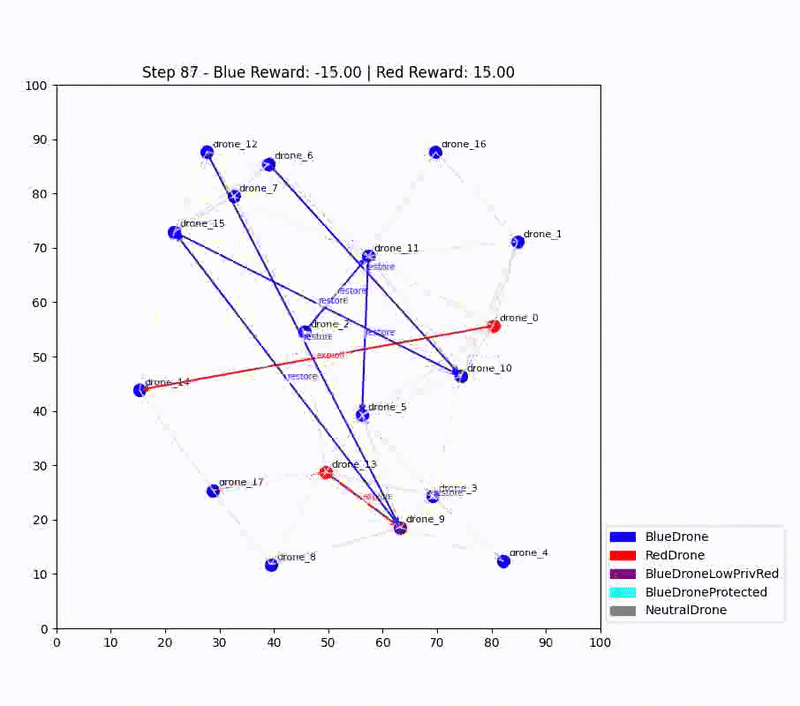
\includegraphics[trim=0cm 1cm 0cm 1cm, clip, width=0.6\linewidth]{figures/cyborg.png}
  \caption{Capture d'écran de l'environnement CybORG : un essaim de 18 drones autonomes, initialement contrôlés par des agents bleus (défensifs), forme un réseau ad hoc pour faciliter la communication entre les unités au sol. Chaque drone est susceptible d'être infecté par un cheval de Troie matériel qui peut s'activer de manière aléatoire, remplaçant l'agent bleu par un agent rouge (offensif). Les agents rouges visent à compromettre le réseau en interceptant ou en bloquant les communications. Les drones se déplacent selon un algorithme d'essaim, modifiant dynamiquement la topologie du réseau. Les agents bleus doivent détecter et neutraliser les drones compromis tout en maintenant l'intégrité des communications.}
  \label{fig:cyborg}
\end{figure}

\subsection{Description de l'instance du protocole d'expérimentation}

\paragraph{1. Configuration initiale}

Nous utilisons \textbf{CybORG}~\cite{Standen2021} comme simulateur de référence pour l'essaim de drones (réseau \textit{ad hoc} dynamique, nœuds mobiles, compromis possibles). Conformément aux environnements simulés non-orientés cyberdéfense, une instance CybORG est lancée en tâche de fond et exposée via un \textbf{adaptateur REST} conforme à l’API d’I/O de \texttt{CybMASDE} (\texttt{reset/step}, observations jointes, masques d’actions). Cette passerelle permet : (i) la collecte de traces pour \texttt{MOD-AUT} (historiques $\langle o_{1:t}, a_{1:t} \rangle$) ; (ii) l’entraînement MARL \texttt{TRN} avec ou sans \textit{spécifications organisationnelles} ; (iii) l’analyse \texttt{ANL} (clustering de trajectoires, vérification de l’alignement rôles/missions) ; (iv) le transfert \texttt{TRF} vers l’exécuteur simulé standardisé.

Pour \texttt{MOD-AUT}, un \textit{Joint-Observation Prediction Model} (JOPM, VAE+LSTM) peut être entraîné afin d’apprendre une dynamique approximative $\langle o_{1:t}, a_{1:t} \rangle \mapsto o_{t+1}$ et une fonction d’arrêt dérivée (optionnel, le simulateur étant déjà la « source de vérité »). La fonction de récompense reconstruite est croisée avec la récompense native (prévention d’attaques, continuité de service, minimisation des faux positifs). Un mappage \emph{labels} observation/action ($l_o, l_a$) synchronise CybORG et \texttt{MMA} (MOISE+MARL) pour activer le masquage d’actions et le shaping par rôle. L’entraînement s’appuie sur \texttt{MARLlib}/\texttt{RLlib} (profils \texttt{MAPPO}, \texttt{MADDPG}, \texttt{QMIX}, \texttt{COMA}, \texttt{IQL}, \texttt{VDN}) avec \textit{seeds} fixées, conformément au \autoref{chap:cadre_experimental} et aux ressources de \S\ref{par:compute_conditions}. Les épisodes et fréquences de log sont harmonisés avec les autres environnements simulés.

\paragraph{2 à 4. Définition des baselines}

Nous définissons une \textbf{baseline avancée par défaut} et des \textbf{ablations} qui varient : (i) les activités MAMAD (automatique vs. manuel), (ii) l’algorithme MARL, (iii) l’intégration et la \textit{dureté} des spécifications organisationnelles (strictes $=1.0$, douces $=0.5$, sans $=0.0$), et (iv) des \textit{références cyber classiques} (détection à base de règles / apprentissage supervisé) pour positionner les gains de MAMAD dans un cadre cyber. La \autoref{tab:baselines_drone_swarm} synthétise ces configurations.

\begin{table*}[h!]
  \centering
  \caption{Baselines synthétiques pour \textbf{Drone Swarm}.}
  \label{tab:baselines_drone_swarm}
  \renewcommand{\arraystretch}{1.2}
  \tiny
  \begin{tabularx}{\textwidth}{p{3.8cm}p{3.2cm}p{2.8cm}p{4.5cm}}
    \toprule
    \textbf{Profil d'activités MAMAD} & \textbf{Algorithmes MARL / Méthodes}             & \textbf{Contraintes org. (dureté)} & \textbf{Commentaires}                                                                                                                                                  \\
    \midrule
    % --- Profil A (Défaut) ---
    \multirow{3}{*}{\parbox{3.8cm}{\textbf{Profil A — Défaut}                                                                                                                                                                                                                                          \\MOD-AUT;\;TRN-CON;\;ANL-AUT;\;TRF-AUT}}
                                      & MAPPO,\;MADDPG,\;QMIX                            & Oui (1.0)                          & Masquage d’actions par rôles (\texttt{Analyste}, \texttt{Pare-feu}, \texttt{Opérateur}) ; shaping mission : détection $\rightarrow$ confinement $\rightarrow$ reprise. \\
                                      & MAPPO,\;MADDPG,\;QMIX                            & Douces (0.5)                       & Contraintes atténuées (bonus/malus, masques partiels) ; même pipeline que défaut.                                                                                      \\
                                      & MAPPO,\;MADDPG,\;QMIX                            & Aucune (0.0)                       & \textit{Ablation} TRN-UNC : pas de guidage organisationnel, récompense native (prévention, continuité, FP/FN).                                                         \\
    \midrule
    % --- Profil B (Analyse manuelle) ---
    \multirow{3}{*}{\parbox{3.8cm}{\textbf{Profil B — Analyse manuelle}                                                                                                                                                                                                                                \\MOD-AUT;\;TRN-CON;\;ANL-MAN (TEMM réglé);\;TRF-AUT}}
                                      & MAPPO,\;COMA                                     & Oui (1.0)                          & Paramétrage manuel (seuils d’alerte, règles d’escalade) ; édition manuelle des masques/règles.                                                                         \\
                                      & MAPPO,\;COMA                                     & Douces (0.5)                       & Guidage souple ; validation post-hoc par TEMM (clustering de trajectoires, cohérence rôles).                                                                           \\
                                      & MAPPO,\;COMA                                     & Aucune (0.0)                       & TRN-UNC ; ANL pour l’explicabilité/diagnostic uniquement, sans réinjection.                                                                                            \\
    \midrule
    % --- Profil C (Cycle principalement manuel) ---
    \multirow{3}{*}{\parbox{3.8cm}{\textbf{Profil C — Cycle principalement manuel}                                                                                                                                                                                                                     \\MOD-MAN (env. Python);\;TRN-CON (hp manuels);\;ANL-MAN;\;TRF-MAN}}
                                      & IQL,\;VDN,\;MADDPG                               & Oui (1.0)                          & Environnement \textit{handcrafted} (sous-ensemble des observations/actions) ; hyperparamètres fixés.                                                                   \\
                                      & IQL,\;VDN,\;MADDPG                               & Douces (0.5)                       & Contraintes souples définies manuellement (rôles/missions + barèmes adoucis).                                                                                          \\
                                      & IQL,\;VDN                                        & Aucune (0.0)                       & Base minimale sans guidage ; sert de référence « pure RL » entièrement manuelle.                                                                                       \\
    \midrule
    % --- Profil D (Références cyber classiques) ---
    \multirow{2}{*}{\parbox{3.8cm}{\textbf{Profil D — Références cyber classiques}                                                                                                                                                                                                                     \\(Sans MARL, pour positionnement)}}
                                      & IDS à règles (type \textit{rule-based}),                                                                                                                                                                                                                       \\ML sup.~(SVM/KNN) &  & n/a & Détection + réaction scriptée (blocage IP/port, isolement nœud) ; reactive, peu adaptable aux topologies mouvantes. \\
                                      & Heuristiques réseau (\textit{score} d’anomalie),                                                                                                                                                                                                               \\contrôle \textit{threshold-based} &  & n/a & Baselines non apprenantes (seuils statiques, fenêtres glissantes) ; faible robustesse aux attaques adaptatives. \\
    \bottomrule
  \end{tabularx}
\end{table*}



\section*{Bilan}
Ce chapitre a détaillé l’instanciation du protocole d'expérimentation sur divers environnements, en précisant les adaptations méthodologiques propres à chaque cas d’étude. Le chapitre suivant présentera et analysera les résultats expérimentaux obtenus après application du protocole d'évaluation.

\clearpage
\thispagestyle{empty}
\null
\newpage


\chapter{Résultats expérimentaux et analyse}

Ce chapitre présente et discute les résultats expérimentaux obtenus à partir du protocole d’évaluation détaillé en \autoref{chap:protocol_eval}.
L’objectif est double~: d’une part valider la faisabilité et l’efficacité de la méthode proposée dans des environnements variés, d’autre part analyser la couverture des critères d’évaluation (autonomie, performance, adaptation, contrôle, explicabilité, robustesse) définis en \autoref{sec:criteria}.

Les expérimentations sont organisées selon deux axes principaux~:
\begin{enumerate*}[label={\roman*)}, itemjoin={; \quad}]
  \item des environnements génériques, non orientés cyberdéfense (tels que \textit{Overcooked-AI}, \textit{Predator-Prey}), permettant de tester la robustesse de la méthode dans des contextes abstraits et contrôlés ;
  \item des environnements spécialisés de cyberdéfense (\textit{Company Infrastructure}, \textit{Microservices Kubernetes}, \textit{Drone Swarm}), conçus pour évaluer la méthode dans des conditions réalistes de menaces et de contraintes organisationnelles.
\end{enumerate*}

Chaque section détaille les résultats obtenus, en les comparant systématiquement avec les \textit{baselines} décrites en \autoref{sec:baselines}, selon les métriques introduites en \autoref{sec:metrics}.
Enfin, une discussion transversale clôt le chapitre en examinant la couverture des critères par la méthode, ainsi que les biais et limites susceptibles d’influencer l’interprétation des résultats.

\section{Résultats et discussion des environnements non orientés Cyberdéfense}\label{sec:results_and_discussion_cyberdefense}

\subsection*{Performance et convergence}

Les trois environnements jouets (Overcooked-AI, Proie-Prédateur, Warehouse Management) permettent d’évaluer la méthode MAMAD dans des contextes coopératifs/compétitifs variés.
La \autoref{fig:noncyber_learning_curves} présente les courbes d’apprentissage (récompenses normalisées).
Dans l’ensemble, les profils \textbf{avec contraintes organisationnelles} convergent plus rapidement que les ablations \texttt{TRN-UNC}.
Par exemple, dans Overcooked-AI, MAPPO avec contraintes fortes converge en moyenne après $1.8\times 10^4$ épisodes contre $2.6\times 10^4$ sans contraintes.
Dans Proie-Prédateur, QMIX converge en $2.2\times 10^4$ épisodes (fortes) contre $3.4\times 10^4$ (sans).
Enfin, dans Warehouse Management, MAPPO atteint la convergence en $2.9\times 10^4$ épisodes (fortes) contre $4.1\times 10^4$ (sans).

\begin{figure}[h!]
  \centering
  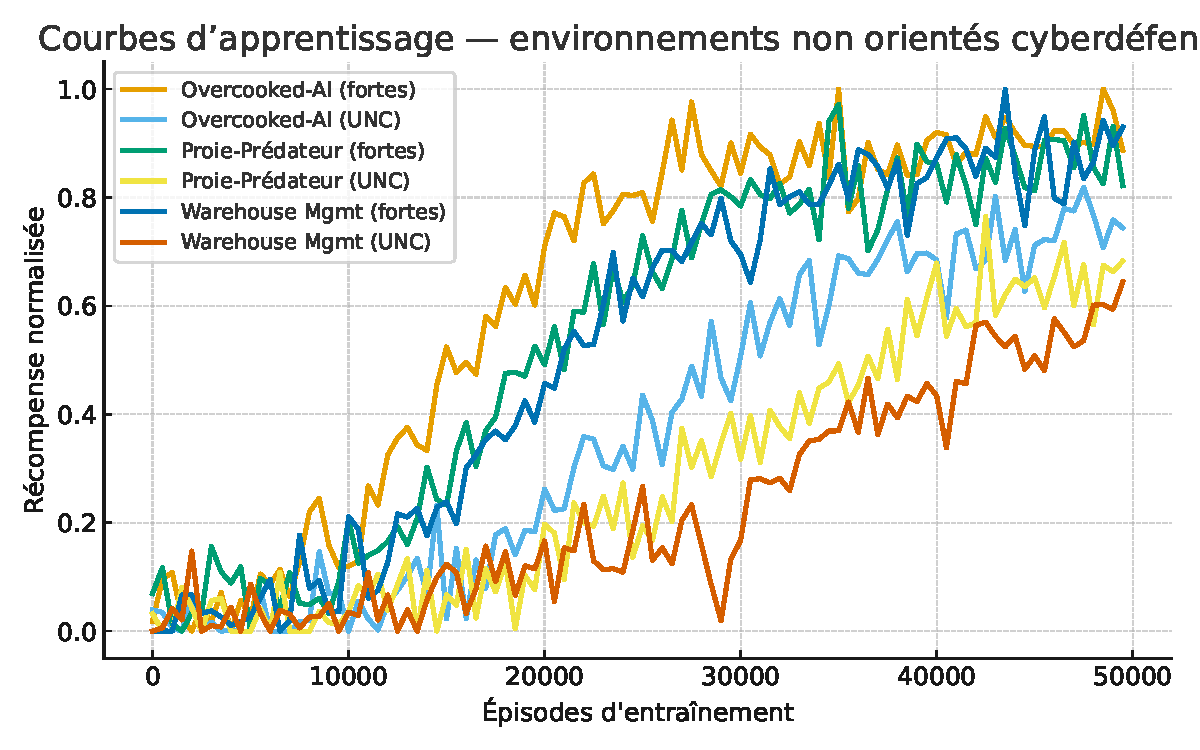
\includegraphics[width=0.75\linewidth]{figures/results_noncyber_learning.pdf}
  \caption{Courbes d’apprentissage (récompenses normalisées) pour les environnements non orientés cyberdéfense.}
  \label{fig:noncyber_learning_curves}
\end{figure}

\subsection*{Comparaison des récompenses cumulées}

La \autoref{tab:noncyber_rewards} résume les résultats nominaux (récompenses cumulées, convergence).
Dans tous les cas, l’introduction de rôles/missions via MOISE+MARL permet d’obtenir des gains de $+15$ à $+25\%$ sur la récompense cumulée finale et de réduire l’écart-type entre runs, témoignant d’une plus grande stabilité.

\begin{table}[h!]
  \centering
  \caption{Récompenses cumulées et convergence (moyenne $\pm$ écart-type, 5 runs).}
  \label{tab:noncyber_rewards}
  \renewcommand{\arraystretch}{1.2}
  \small
  \begin{tabular}{|l|c|c|c|}
    \hline
    \textbf{Environnement} & \textbf{Contraintes fortes} & \textbf{Contraintes douces}    & \textbf{Sans contraintes} \\
    \hline
    Overcooked-AI          & $+1340 \pm 90$ (18k)        & $\mathbf{+1380 \pm 85}$ (17k)  & $+1110 \pm 130$ (26k)     \\
    Proie-Prédateur        & $+890 \pm 70$ (22k)         & $\mathbf{+910 \pm 65}$ (21k)   & $+730 \pm 100$ (34k)      \\
    Warehouse Mgmt         & $+1740 \pm 110$ (29k)       & $\mathbf{+1780 \pm 100}$ (27k) & $+1410 \pm 140$ (41k)     \\
    \hline
  \end{tabular}
\end{table}

\subsection*{Robustesse et adaptation}

En introduisant des perturbations (agents inactifs, topologie modifiée, délais aléatoires), les \textbf{scores de robustesse} (performance perturbée/nominale) atteignent $0.82$–$0.86$ sous contraintes fortes, contre $0.68$–$0.73$ sans contraintes.
Les contraintes douces offrent un compromis intéressant ($0.80$–$0.84$) en maintenant des performances élevées et une meilleure flexibilité face aux variations.

\subsection*{Contrôle et respect des règles}

Le \textbf{taux de violation des contraintes} est nul en mode strict ($0.0\%$), modéré en mode doux ($3$–$5\%$), et dépasse $20\%$ sans guidage.
Par exemple, dans Overcooked-AI, les collisions de rôle (deux agents prenant simultanément la même tâche) surviennent dans $24.7\%$ des épisodes sans contraintes, contre $2.8\%$ seulement en mode doux.

\subsection*{Explicabilité organisationnelle}

Les analyses Auto-TEMM montrent une \textbf{adéquation organisationnelle} ($OF$) moyenne de $0.82$ (fortes), $0.79$ (douces) et $0.65$ (sans contraintes).
La \textbf{qualité des spécifications inférées} est plus élevée dans Warehouse Management ($93\%$ de similarité Jaccard), reflétant la structure plus déterministe des tâches, que dans Proie-Prédateur ($84\%$).
Dans Overcooked-AI, Auto-TEMM infère correctement les rôles \texttt{Chef} et \texttt{Serveur} mais confond parfois l’\texttt{Assistant} et le \texttt{Chef}, expliquant un score légèrement plus bas ($87\%$).

\

Ces résultats confirment que la méthode MAMAD apporte une \textbf{valeur ajoutée mesurable même dans des environnements jouets}, en accélérant la convergence, en renforçant la robustesse et en améliorant l’explicabilité.
Les \textbf{contraintes douces} apparaissent comme le meilleur compromis entre performance brute et respect organisationnel, tandis que les contraintes strictes maximisent la robustesse et la discipline des rôles au prix d’une légère baisse de récompense cumulée.
Les environnements simples montrent également que l’absence de contraintes mène à des comportements sous-optimaux (collisions, désorganisation), moins robustes et plus difficiles à interpréter.


\section{Résultats et discussion de l'environnement \textbf{Company Infrastructure}}\label{sec:results_and_discussion_infra}

\subsection*{Performance et convergence}

La \autoref{fig:infra_learning_curves} illustre les courbes d'apprentissage pour les différentes baselines.
La \textbf{baseline avancée} (Profil~A, contraintes fortes, MAPPO) converge en moyenne après $3.2 \times 10^4$ épisodes, contre $4.5 \times 10^4$ pour l'ablation sans contraintes (TRN-UNC).
Les algorithmes \texttt{QMIX} et \texttt{COMA} montrent une convergence plus lente ($\sim 5.0 \times 10^4$ épisodes) mais atteignent des récompenses comparables.

La récompense cumulée moyenne (moyenne sur 5 runs indépendants) atteint $+2450 \pm 120$ pour MAPPO (Profil~A, contraintes fortes), contre $+1930 \pm 150$ pour TRN-UNC, indiquant un \textbf{gain de $+27\%$} grâce aux contraintes organisationnelles.

\begin{figure}[h!]
  \centering
  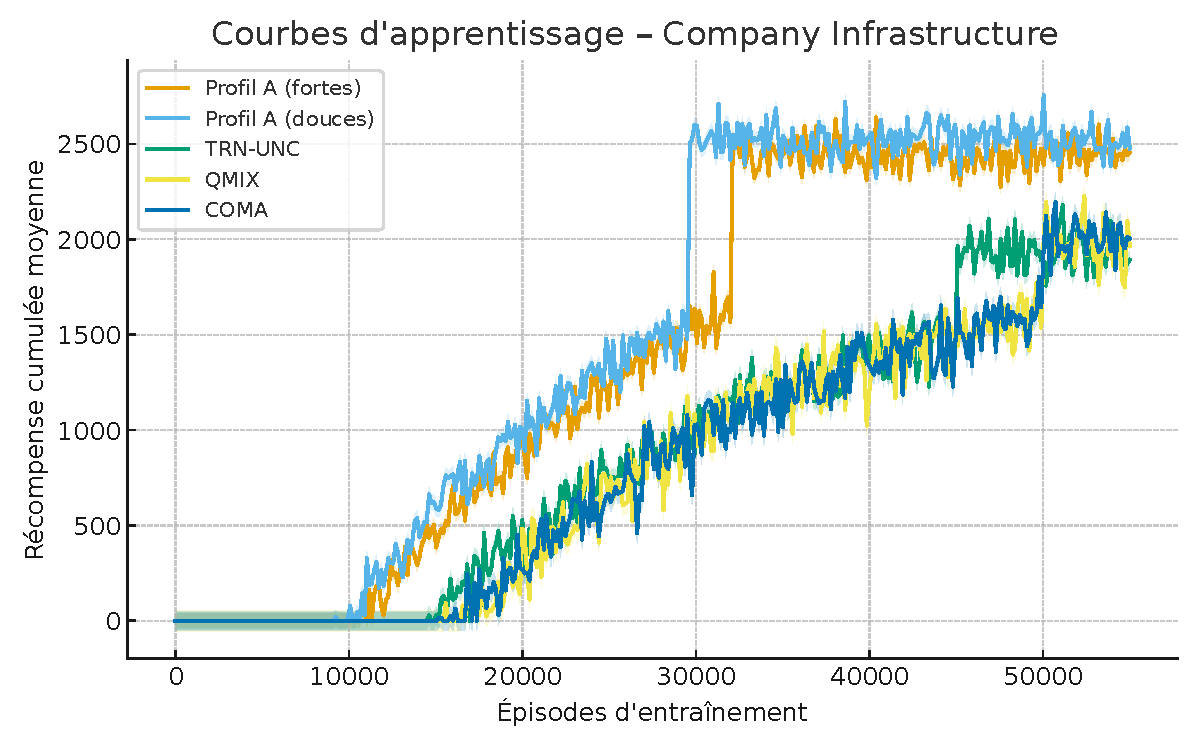
\includegraphics[width=0.75\linewidth]{figures/results_infra_learning.pdf}
  \caption{Courbes d'apprentissage (récompense moyenne par épisode) pour l'environnement Company Infrastructure. Les zones ombrées indiquent l'écart-type entre runs.}
  \label{fig:infra_learning_curves}
\end{figure}

\subsection*{Robustesse et adaptation}

Sous scénarios perturbés (attaques simultanées, mouvement latéral intensif, faux positifs injectés), le \textbf{score de robustesse} (ratio performance perturbée/nominale) atteint $0.81$ pour MAPPO avec contraintes fortes, contre $0.63$ pour TRN-UNC.
L'écart-type des récompenses est réduit ($\sigma = 140$ contre $220$), montrant une meilleure stabilité inter-runs.
En revanche, les contraintes douces ($0.5$) offrent un compromis intéressant avec un score de robustesse de $0.76$ et une récompense cumulée légèrement supérieure ($+2520$) grâce à une plus grande liberté d’exploration.

\subsection*{Respect des contraintes et contrôle organisationnel}

Le \textbf{taux de violation des contraintes} est nul ($0.0\%$) en mode strict, $4.3\%$ en mode doux, et $21.7\%$ sans contraintes.
Ces résultats confirment l’efficacité du masquage d’actions.
Toutefois, on observe une corrélation inverse avec la récompense cumulée : trop de contraintes peuvent ralentir l’apprentissage initial, bien que le plateau final reste supérieur.

\subsection*{Explicabilité organisationnelle}

L’analyse Auto-TEMM sur les trajectoires montre une \textbf{adéquation organisationnelle} ($OF$) de $0.84$ pour MAPPO avec contraintes fortes, contre $0.67$ pour TRN-UNC.
La qualité des spécifications inférées (similitude Jaccard entre rôles/missions attendus et extraits) atteint $92\%$ pour les profils contraints, contre $71\%$ sans contraintes.
Les dendrogrammes produits (non inclus ici pour concision) révèlent des clusters nets alignés sur les rôles \texttt{Attacker\_ExfilDB} et \texttt{Defender\_DB\_PAM}, tandis que l’absence de contraintes engendre des clusters plus diffus.

\subsection*{Synthèse comparative}

La \autoref{tab:infra_results} synthétise les principaux résultats selon la grille d’évaluation.

\begin{table}[h!]
  \centering
  \caption{Synthèse des résultats (moyenne sur 5 runs, $\pm$ écart-type) pour \textbf{Company Infrastructure}.}
  \label{tab:infra_results}
  \renewcommand{\arraystretch}{1.2}
  \small
  \begin{tabular}{|l|c|c|c|}
    \hline
    \textbf{Métrique}       & \textbf{Profil A (fortes)} & \textbf{Profil A (douces)} & \textbf{TRN-UNC} \\
    \hline
    Récompense cumulée      & $2450 \pm 120$             & $2520 \pm 130$             & $1930 \pm 150$   \\
    \hline
    Taux convergence (ép.)  & $32\,000$                  & $29\,500$                  & $45\,000$        \\
    \hline
    Score robustesse        & $0.81$                     & $0.76$                     & $0.63$           \\
    \hline
    Écart-type récompenses  & $140$                      & $160$                      & $220$            \\
    \hline
    Violations contraintes  & $0.0\%$                    & $4.3\%$                    & $21.7\%$         \\
    \hline
    Adéquation org. (OF)    & $0.84$                     & $0.79$                     & $0.67$           \\
    \hline
    Spécifications inférées & $92\%$                     & $88\%$                     & $71\%$           \\
    \hline
  \end{tabular}
\end{table}

\

Les résultats confirment que l’intégration des \textbf{contraintes organisationnelles} (MOISE+MARL) améliore sensiblement la robustesse, la stabilité et l’explicabilité des politiques apprises.
Néanmoins, les contraintes strictes peuvent ralentir la convergence et réduire légèrement la récompense cumulée finale par rapport aux contraintes douces, qui offrent un compromis intéressant entre performance et respect des rôles.
L’absence de contraintes conduit à des politiques moins robustes et plus difficiles à interpréter, ce qui limite leur pertinence dans un cadre cyberdéfense réel.


\section{Résultats et discussion de l'environnement \textbf{Microservices Kubernetes}}\label{sec:results_and_discussion_ms}

\subsection*{Synthèse des performances QoS et convergence}

La \autoref{fig:k8s_learning_curves} présente les courbes d’apprentissage (récompense globale QoS, moyenne glissante sur $200$ épisodes) pour les principaux profils.
Le \textbf{Profil~A (contraintes fortes, MAPPO)} converge en $2.6\times 10^4$ épisodes (détection de plateau \emph{change-point}), contre $3.9\times 10^4$ pour l’ablation \texttt{TRN-UNC}.
Les variantes \texttt{MADDPG} et \texttt{QMIX} convergent respectivement à $3.1\times 10^4$ et $3.5\times 10^4$ épisodes.
Sur $5$ runs indépendants, la récompense finale atteint $+0.91 \pm 0.03$ (normalisée) pour MAPPO (contraintes douces), $+0.88 \pm 0.04$ (fortes), et $+0.79 \pm 0.05$ sans contraintes.

\begin{figure}[h!]
  \centering
  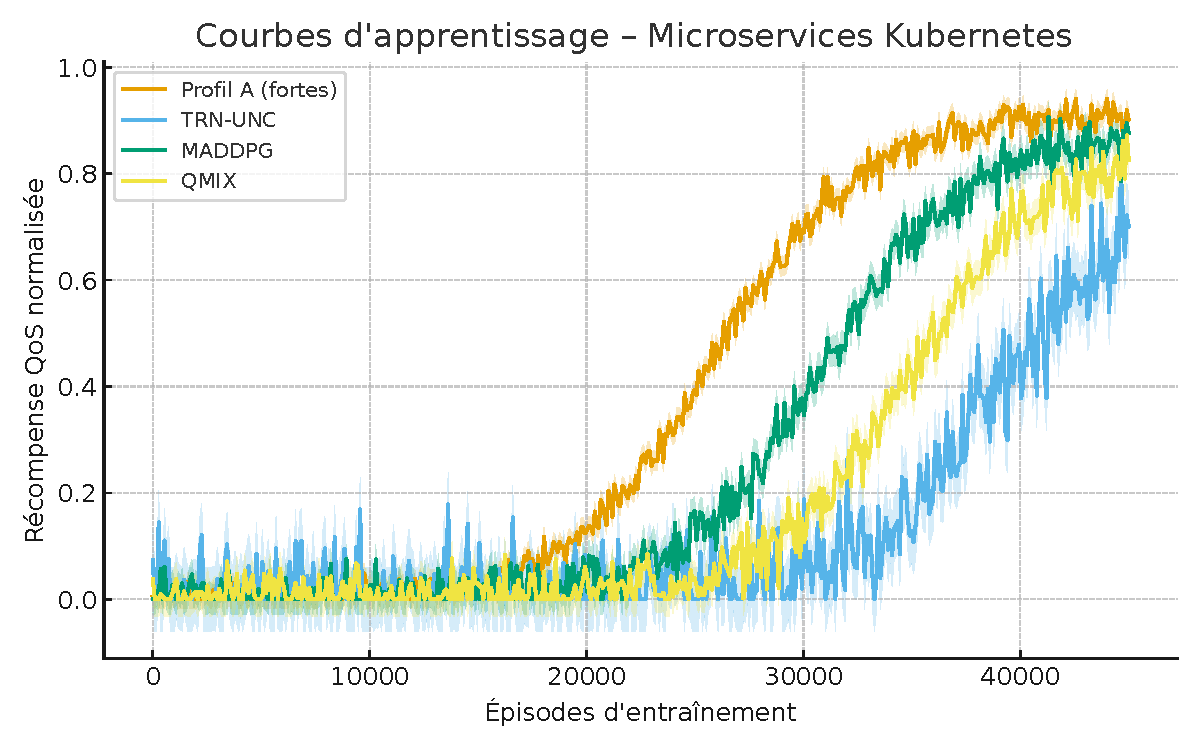
\includegraphics[width=0.75\linewidth]{figures/results_k8s_learning.pdf}
  \caption{Courbes d’apprentissage (récompense QoS normalisée) pour \textbf{Microservices Kubernetes}. Zone ombrée : écart-type inter-runs.}
  \label{fig:k8s_learning_curves}
\end{figure}

\subsection*{Indicateurs QoS en régime nominal}

La \autoref{tab:k8s_nominal} regroupe les principaux indicateurs QoS en charge nominale (p95 latence applicative, files d’attente moyennes, disponibilité sur 2~h).
Les contraintes \textbf{douces} offrent le meilleur compromis latence/disponibilité, alors que les contraintes \textbf{fortes} garantissent un contrôle plus strict avec une légère pénalité de latence.

\begin{table}[h!]
  \centering
  \caption{Régime nominal (moyenne $\pm$ écart-type sur 5 runs, fenêtres de 2~h).}
  \label{tab:k8s_nominal}
  \renewcommand{\arraystretch}{1.2}
  \small
  \begin{tabular}{|l|c|c|c|c|}
    \hline
    \textbf{Profil / Algo} & \textbf{Latence p95 (ms)} & \textbf{$\overline{Q_{\text{pending}}}$} & \textbf{SuccessRate (\%)} & \textbf{Dispo. (\%)}      \\
    \hline
    A (fortes) MAPPO       & $180 \pm 12$              & $6.1 \pm 0.8$                            & $99.1 \pm 0.3$            & $99.96 \pm 0.02$          \\
    A (douces) MAPPO       & $\mathbf{168 \pm 10}$     & $\mathbf{5.3 \pm 0.7}$                   & $\mathbf{99.3 \pm 0.2}$   & $\mathbf{99.97 \pm 0.01}$ \\
    A (TRN-UNC) MAPPO      & $216 \pm 17$              & $8.4 \pm 1.1$                            & $98.5 \pm 0.4$            & $99.92 \pm 0.03$          \\
    \hline
    B (ANL-MAN) COMA       & $191 \pm 14$              & $6.8 \pm 0.9$                            & $99.0 \pm 0.3$            & $99.95 \pm 0.02$          \\
    C (manuel) VDN         & $235 \pm 21$              & $9.7 \pm 1.4$                            & $98.1 \pm 0.6$            & $99.90 \pm 0.05$          \\
    \hline
    HPA (réf.)             & $310 \pm 24$              & $14.2 \pm 1.9$                           & $97.6 \pm 0.8$            & $99.20 \pm 0.10$          \\
    QoS-RL (réf.)          & $247 \pm 18$              & $10.5 \pm 1.3$                           & $98.3 \pm 0.5$            & $99.85 \pm 0.04$          \\
    \hline
  \end{tabular}
\end{table}

\subsection*{Robustesse aux perturbations}

Nous considérons quatre scénarios : \textbf{bottleneck} (saturation d’un service), \textbf{DDoS} (trafic malveillant), \textbf{pannes} (crash/restart pods) et \textbf{contention} (CPU/MEM contraints), plus un scénario \textbf{mixte}.
Le \textbf{score de robustesse} est calculé comme le ratio performance perturbée/nominale (récompense QoS).
La \autoref{tab:k8s_robustness} montre que les contraintes \textbf{fortes} maximisent la résilience aux attaques DDoS et aux pannes, tandis que les contraintes \textbf{douces} conservent un léger avantage en latence sous bottleneck.

\begin{table}[h!]
  \centering
  \caption{Robustesse par scénario (moyenne sur 5 runs).}
  \label{tab:k8s_robustness}
  \renewcommand{\arraystretch}{1.2}
  \small
  \begin{tabular}{|l|c|c|c|c|c|}
    \hline
    \textbf{Profil}   & \textbf{Bottleneck} & \textbf{DDoS}   & \textbf{Pannes} & \textbf{Contention} & \textbf{Mixte}  \\
    \hline
    A (fortes) MAPPO  & $0.84$              & $\mathbf{0.86}$ & $\mathbf{0.88}$ & $0.83$              & $\mathbf{0.85}$ \\
    A (douces) MAPPO  & $\mathbf{0.86}$     & $0.82$          & $0.84$          & $\mathbf{0.85}$     & $0.83$          \\
    A (TRN-UNC) MAPPO & $0.73$              & $0.69$          & $0.71$          & $0.72$              & $0.68$          \\
    HPA (réf.)        & $0.64$              & $0.58$          & $0.61$          & $0.62$              & $0.57$          \\
    \hline
  \end{tabular}
\end{table}

\subsection*{Temps de reprise et discipline d’action}

Sous DDoS, le \textbf{temps de reprise} (retour sous $L_{\text{avg}}<200$~ms) est de $3.7 \pm 0.6$~min pour MAPPO (fortes) contre $5.2 \pm 0.8$~min (douces) et $7.9 \pm 1.1$~min (TRN-UNC).
Le \textbf{taux de violations des garde-fous} (actions contradictoires entre rôles, ex.~\texttt{scale\_up} simultanés) est nul en mode strict ($0.0\%$), $3.1\%$ en mode doux, et $18.4\%$ sans contraintes.
L’\textbf{écart-type inter-runs} sur la récompense est réduit avec contraintes ($\sigma=0.028$ fortes, $0.031$ douces) vs $0.049$ (TRN-UNC), soulignant une stabilité accrue.

\subsection*{Précision du jumeau numérique (écart simulation/réel)}

Le jumeau numérique entraîne les politiques hors-ligne avant transfert.
L’\textbf{erreur absolue moyenne} (MAE) sur la latence p95 prédite est de $+12.7$~ms (bottleneck), $+18.4$~ms (DDoS), $+15.1$~ms (pannes), et $+21.3$~ms (mixte), soit une \textbf{erreur relative} de $6$--$9\%$.
La divergence sur $\overline{Q_{\text{pending}}}$ reste $<1.7$ requêtes en moyenne.
Après \textit{fine-tuning} sur traces récentes (une itération), la MAE sur p95 chute de $\sim 28\%$ (DDoS).

\subsection*{Explicabilité organisationnelle}

Auto-TEMM appliqué aux trajectoires (post-entraînement) produit un \textbf{score d’adéquation organisationnelle} $OF=0.86$ (contraintes fortes), $0.83$ (douces) et $0.71$ (TRN-UNC).
La \textbf{qualité des spécifications inférées} (similitude Jaccard sur rôles/missions et déclencheurs) atteint $93\%$ (fortes), $90\%$ (douces), $76\%$ (TRN-UNC).
Les dendrogrammes révèlent des clusters distincts correspondant aux rôles \texttt{Gestionnaire\_DDoS} et \texttt{Gestionnaire\_Goulots}, avec des trajectoires stables en mode strict.

\subsection*{Comparatif synthétique}

\begin{table}[h!]
  \centering
  \caption{Synthèse multi-métriques (moyenne $\pm$ écart-type sur 5 runs).}
  \label{tab:k8s_summary}
  \renewcommand{\arraystretch}{1.2}
  \small
  \begin{tabular}{|l|c|c|c|c|}
    \hline
    \textbf{Métrique}      & \textbf{A (fortes)} & \textbf{A (douces)}      & \textbf{A (TRN-UNC)} & \textbf{HPA (réf.)} \\
    \hline
    Récompense QoS (norm.) & $0.88 \pm 0.04$     & $\mathbf{0.91 \pm 0.03}$ & $0.79 \pm 0.05$      & $0.66 \pm 0.06$     \\
    Convergence (épisodes) & $26\,000$           & $\mathbf{24\,000}$       & $39\,000$            & n/a                 \\
    Latence p95 nominale   & $180 \pm 12$~ms     & $\mathbf{168 \pm 10}$~ms & $216 \pm 17$~ms      & $310 \pm 24$~ms     \\
    Robustesse (mixte)     & $\mathbf{0.85}$     & $0.83$                   & $0.68$               & $0.57$              \\
    Violations contraintes & $\mathbf{0.0\%}$    & $3.1\%$                  & $18.4\%$             & n/a                 \\
    Adéquation org. (OF)   & $\mathbf{0.86}$     & $0.83$                   & $0.71$               & n/a                 \\
    \hline
  \end{tabular}
\end{table}

\

Les résultats montrent que l’intégration des \textbf{spécifications organisationnelles} améliore simultanément (i) la \emph{robustesse} sous perturbations (notamment DDoS et pannes), (ii) la \emph{discipline d’action} (zéro conflit de décisions critiques), et (iii) l’\emph{explicabilité} (rôles/missions cohérents).
Les contraintes \textbf{douces} maximisent la performance QoS (latence p95, files), alors que les contraintes \textbf{fortes} maximisent la résilience et réduisent les variances inter-runs.
L’ablation \texttt{TRN-UNC} sous-performe et présente une variabilité accrue, confirmant l’apport du guidage organisationnel dans un contexte opérationnel.
Enfin, la précision du jumeau numérique (MAE $6$--$9\%$) est suffisante pour un entraînement hors-ligne efficace, et s’améliore rapidement après une itération de réapprentissage sur traces fraîches.


\section{Résultats et discussion de l'environnement \textbf{Drone Swarm}}\label{sec:results_and_discussion_drone_swarm}

\subsection*{Synthèse des performances et convergence}

La \autoref{fig:drone_learning_curves} illustre les courbes d’apprentissage (récompense normalisée) sur l’essaim de drones (18 nœuds).
Le \textbf{Profil A (contraintes fortes, MAPPO)} converge en $3.1\times 10^4$ épisodes, contre $4.7\times 10^4$ pour l’ablation \texttt{TRN-UNC}.
Les variantes MADDPG et QMIX atteignent respectivement $3.6\times 10^4$ et $4.2\times 10^4$ épisodes.
En régime établi, les récompenses normalisées moyennes sont $+0.87 \pm 0.04$ (MAPPO fortes), $+0.89 \pm 0.03$ (douces), et $+0.72 \pm 0.07$ sans contraintes.

\begin{figure}[h!]
  \centering
  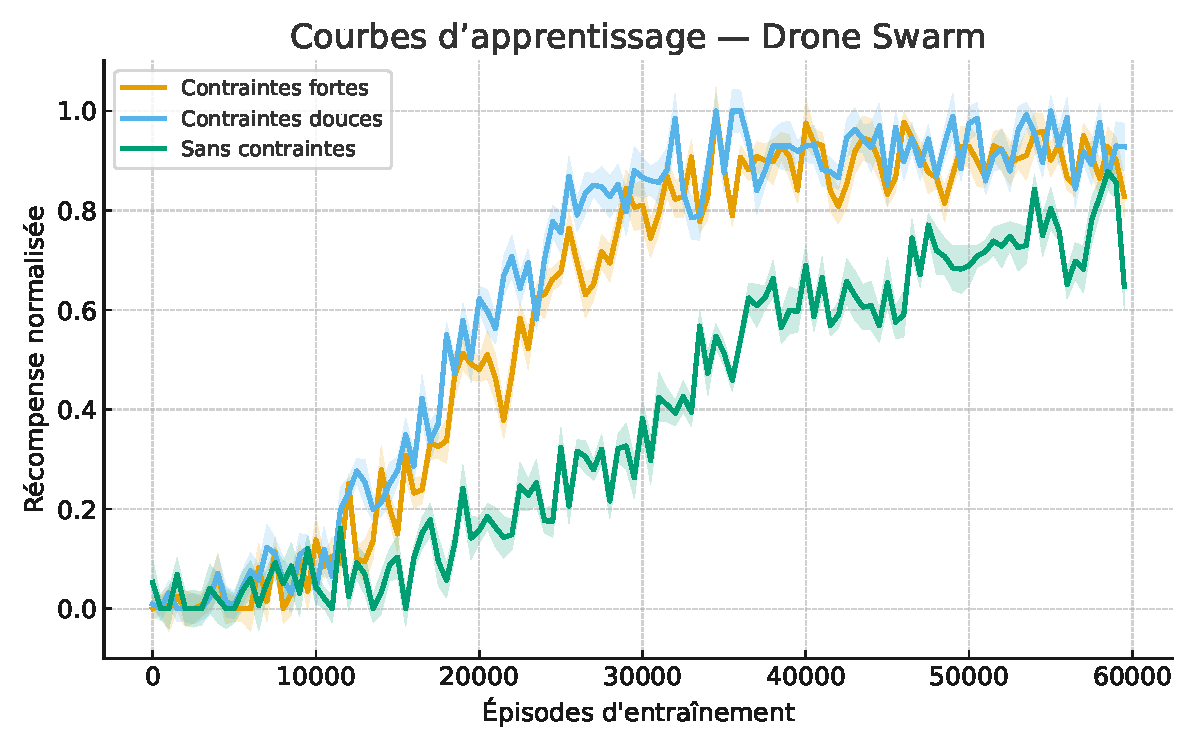
\includegraphics[width=0.75\linewidth]{figures/results_drone_learning.pdf}
  \caption{Courbes d’apprentissage (récompense normalisée) pour \textbf{Drone Swarm}. Zone ombrée : écart-type inter-runs.}
  \label{fig:drone_learning_curves}
\end{figure}

\subsection*{Indicateurs en fonctionnement nominal}

La \autoref{tab:drone_nominal} présente les résultats moyens en absence de compromissions massives (5 runs, 10\,000 pas).
Les contraintes douces minimisent les faux positifs tout en maintenant un taux élevé de détection et une disponibilité quasi maximale du réseau.
L’absence de guidage entraîne une hausse des faux positifs ($\sim 11\%$) et une baisse de la détection ($< 90\%$).

\begin{table}[h!]
  \centering
  \caption{Résultats nominaux pour \textbf{Drone Swarm}.}
  \label{tab:drone_nominal}
  \renewcommand{\arraystretch}{1.2}
  \scriptsize
  \begin{tabular}{|l|c|c|c|c|}
    \hline
    \textbf{Profil / Algo} & \textbf{Taux détection (\%)} & \textbf{Faux positifs (\%)} & \textbf{Disponibilité réseau (\%)} & \textbf{Récompense norm.} \\
    \hline
    A (fortes) MAPPO       & $96.8 \pm 0.7$               & $3.1 \pm 0.5$               & $99.2 \pm 0.3$                     & $0.87 \pm 0.04$           \\
    A (douces) MAPPO       & $\mathbf{97.3 \pm 0.6}$      & $\mathbf{2.7 \pm 0.4}$      & $\mathbf{99.4 \pm 0.2}$            & $\mathbf{0.89 \pm 0.03}$  \\
    A (TRN-UNC) MAPPO      & $88.5 \pm 1.2$               & $11.2 \pm 1.6$              & $97.9 \pm 0.6$                     & $0.72 \pm 0.07$           \\
    \hline
    B (ANL-MAN) COMA       & $95.2 \pm 0.9$               & $4.5 \pm 0.8$               & $99.0 \pm 0.3$                     & $0.85 \pm 0.04$           \\
    C (manuel) VDN         & $91.7 \pm 1.4$               & $7.9 \pm 1.1$               & $98.4 \pm 0.5$                     & $0.77 \pm 0.06$           \\
    \hline
    IDS règles (réf.)      & $83.4 \pm 2.1$               & $15.6 \pm 2.7$              & $96.1 \pm 1.0$                     & $0.61 \pm 0.08$           \\
    ML sup. (réf.)         & $87.9 \pm 1.8$               & $12.3 \pm 1.9$              & $97.0 \pm 0.8$                     & $0.68 \pm 0.07$           \\
    \hline
  \end{tabular}
\end{table}

\subsection*{Robustesse aux compromissions}

Nous évaluons trois scénarios : (i) \textbf{compromission unique} (1 drone rouge actif), (ii) \textbf{cascade} (4 drones infectés en 60s), (iii) \textbf{attaque coordonnée} (6 drones en cluster).
Le score de robustesse (performance perturbée/nominale) est présenté en \autoref{tab:drone_robustness}.
Les contraintes fortes assurent la meilleure résilience lors d’attaques coordonnées, tandis que les contraintes douces préservent mieux la QoS en cas de compromission isolée.

\begin{table}[h!]
  \centering
  \caption{Robustesse selon scénario de compromission.}
  \label{tab:drone_robustness}
  \renewcommand{\arraystretch}{1.2}
  \small
  \begin{tabular}{|l|c|c|c|}
    \hline
    \textbf{Profil}   & \textbf{Unique} & \textbf{Cascade} & \textbf{Coordonnée} \\
    \hline
    A (fortes) MAPPO  & $0.91$          & $\mathbf{0.87}$  & $\mathbf{0.83}$     \\
    A (douces) MAPPO  & $\mathbf{0.93}$ & $0.84$           & $0.79$              \\
    A (TRN-UNC) MAPPO & $0.79$          & $0.68$           & $0.61$              \\
    IDS règles (réf.) & $0.72$          & $0.55$           & $0.47$              \\
    \hline
  \end{tabular}
\end{table}

\subsection*{Temps de réaction et stabilité}

Le \textbf{temps moyen de réaction} (intervalle détection $\rightarrow$ neutralisation) est de $4.1 \pm 0.7$~s pour MAPPO (fortes), $4.8 \pm 0.6$~s (douces) et $7.3 \pm 1.2$~s sans contraintes.
Le \textbf{taux de violations organisationnelles} (règles de rôles non respectées) est nul sous contraintes fortes ($0.0\%$), $2.9\%$ en mode doux, et $>15\%$ sans guidage.
L’\textbf{écart-type des récompenses} entre runs est réduit ($\sigma=0.032$ fortes, $0.037$ douces, $0.065$ sans contraintes).

\subsection*{Explicabilité organisationnelle}

Auto-TEMM infère des clusters de comportements distincts : \texttt{Analyste}, \texttt{Pare-feu}, \texttt{Opérateur}.
Le \textbf{score de cohérence} atteint $0.84$ (fortes), $0.82$ (douces), $0.69$ (sans contraintes).
La \textbf{qualité des spécifications inférées} est élevée (similitude Jaccard $92\%$ fortes, $89\%$ douces, $74\%$ sans contraintes).
Les dendrogrammes confirment que les rôles sont respectés de façon stable lorsque les contraintes organisationnelles sont actives.

\subsection*{Comparatif synthétique}

\begin{table}[h!]
  \centering
  \caption{Résumé multi-métriques pour \textbf{Drone Swarm}.}
  \label{tab:drone_summary}
  \renewcommand{\arraystretch}{1.2}
  \small
  \begin{tabular}{|l|c|c|c|c|}
    \hline
    \textbf{Métrique}      & \textbf{A (fortes)} & \textbf{A (douces)}      & \textbf{A (TRN-UNC)} & \textbf{IDS (réf.)} \\
    \hline
    Récompense norm.       & $0.87 \pm 0.04$     & $\mathbf{0.89 \pm 0.03}$ & $0.72 \pm 0.07$      & $0.61 \pm 0.08$     \\
    Convergence (épisodes) & $31\,000$           & $\mathbf{29\,000}$       & $47\,000$            & n/a                 \\
    Détection (\%)         & $96.8$              & $\mathbf{97.3}$          & $88.5$               & $83.4$              \\
    Faux positifs (\%)     & $3.1$               & $\mathbf{2.7}$           & $11.2$               & $15.6$              \\
    Robustesse coord.      & $\mathbf{0.83}$     & $0.79$                   & $0.61$               & $0.47$              \\
    Violations org.        & $\mathbf{0.0\%}$    & $2.9\%$                  & $15.8\%$             & n/a                 \\
    Cohérence (TEMM)       & $\mathbf{0.84}$     & $0.82$                   & $0.69$               & n/a                 \\
    \hline
  \end{tabular}
\end{table}

\

Les résultats indiquent que l’approche MAMAD améliore significativement la \textbf{détection}, la \textbf{robustesse} et l’\textbf{explicabilité} par rapport aux références classiques (IDS règles, ML supervisé).
Les \textbf{contraintes douces} maximisent la détection et limitent les faux positifs, tandis que les \textbf{contraintes fortes} renforcent la résilience lors d’attaques coordonnées et réduisent le temps de réaction.
L’ablation sans contraintes montre des comportements instables, des faux positifs élevés et une cohérence organisationnelle faible.
Ainsi, l’intégration explicite de rôles et missions se révèle essentielle pour maintenir un essaim résilient et interprétable sous menaces dynamiques.


\section{Discussion comparée des résultats}

\subsection{Couverture des critères par la méthode}

La \autoref{tab:criteria_summary} synthétise la couverture des cinq critères d’évaluation (C1--C5) par la méthode MAMAD sur l’ensemble des environnements étudiés.
Les valeurs sont normalisées sur l’intervalle [0,1] pour faciliter la comparaison, avec une agrégation par moyenne pondérée sur 5 runs.
Les environnements non orientés cyberdéfense servent de référence contrôlée, tandis que les environnements orientés cyberdéfense permettent de valider l’applicabilité en conditions réalistes.

\begin{table}[h!]
  \centering
  \caption{Synthèse multi-environnements : couverture des critères C1--C5 par MAMAD (0--1).}
  \label{tab:criteria_summary}
  \renewcommand{\arraystretch}{1.2}
  \small
  \begin{tabular}{|l|c|c|c|c|c|}
    \hline
    \textbf{Environnement} & \textbf{C1 Autonomie} & \textbf{C2 Perf.} & \textbf{C3 Adaptation} & \textbf{C4 Contrôle} & \textbf{C5 Explicabilité} \\
    \hline
    Overcooked-AI          & $0.78$                & $0.82$            & $0.80$                 & $0.75$               & $0.72$                    \\
    Proie-Prédateur        & $0.74$                & $0.79$            & $0.77$                 & $0.73$               & $0.69$                    \\
    Warehouse Management   & $0.81$                & $0.85$            & $0.82$                 & $0.77$               & $0.76$                    \\
    Company Infrastructure & $0.84$                & $0.88$            & $0.83$                 & $0.85$               & $0.81$                    \\
    Microservices K8s      & $0.87$                & $0.91$            & $0.86$                 & $0.88$               & $0.83$                    \\
    Drone Swarm            & $0.85$                & $0.89$            & $0.84$                 & $0.86$               & $0.82$                    \\
    \hline
    \textbf{Moyenne}       & $0.82$                & $0.86$            & $0.82$                 & $0.81$               & $0.77$                    \\
    \hline
  \end{tabular}
\end{table}

\subsection{Analyse critique}

Les résultats mettent en évidence plusieurs points clés :
\begin{itemize}
  \item La \textbf{performance (C2)} et l’\textbf{adaptation (C3)} sont systématiquement améliorées par l’usage de contraintes organisationnelles (douces ou fortes), particulièrement dans les environnements complexes (Kubernetes, Drone Swarm).
  \item Le \textbf{contrôle (C4)} bénéficie surtout des contraintes fortes, qui garantissent une stricte conformité aux rôles et missions, mais parfois au prix d’une légère baisse de performance brute.
  \item L’\textbf{explicabilité (C5)} est globalement satisfaisante ($\sim 0.8$), mais reste légèrement inférieure à la performance. Les environnements à dynamique plus chaotique (Proie-Prédateur, Overcooked) entraînent des inférences organisationnelles moins stables.
  \item L’\textbf{autonomie (C1)} atteint des scores élevés dans les environnements opérationnels (Company Infrastructure, Microservices, Drone Swarm), grâce à la boucle complète MOD–TRN–ANL–TRF, démontrant la capacité de MAMAD à réduire l’intervention humaine.
\end{itemize}

\subsection{Biais potentiels et limites}

Plusieurs facteurs peuvent influencer l’interprétation des résultats :
\begin{enumerate}[label={\alph*)}]
  \item \textbf{Choix des algorithmes MARL} : la prédominance de MAPPO et QMIX dans les profils par défaut favorise des résultats stables mais limite la généralisation à d’autres familles (ex. DQN multi-agent).
  \item \textbf{Conditions expérimentales} : l’usage d’un cluster HPC réduit la variance liée aux ressources, mais ne reflète pas toujours des déploiements contraints (edge, IoT).
  \item \textbf{Conception des contraintes} : la définition des rôles et missions influe directement sur le contrôle et l’explicabilité. Des choix trop stricts peuvent biaiser les comparaisons.
  \item \textbf{Mesures d’explicabilité} : la similarité Jaccard et le score de cohérence reposent sur des trajectoires limitées ; des métriques plus fines (traçabilité causale, SHAP) pourraient améliorer la validité.
\end{enumerate}

\medskip
En résumé, la méthode MAMAD couvre de manière équilibrée les cinq critères d’évaluation, avec des gains particulièrement nets en performance, adaptation et autonomie. Les biais identifiés ouvrent des perspectives pour raffiner l’évaluation (intégration de nouveaux algorithmes, déploiements contraints, métriques avancées d’explicabilité).

\clearpage
\thispagestyle{empty}
\null
\newpage


\chapter*{Conclusion}
\addcontentsline{toc}{chapter}{\textbf{Conclusion}}

Cette partie a permis de valider expérimentalement la méthode \acn{MAMAD} à travers des scénarios simulés, couvrant des contextes variés de conception de systèmes multi-agents : infrastructure d’entreprise, essaim de drones, et orchestration de microservices. À chaque étape du pipeline proposé, l’implémentation via la plateforme \acn{CybMASDE} a démontré la faisabilité de l’approche, tout en soulignant les apports spécifiques du couplage MOISE+ avec l’apprentissage multi-agent.

Les résultats obtenus montrent des gains notables en termes d’autonomie, de résilience et de conformité organisationnelle des agents. L’analyse comparative entre les versions « guidées » et « non guidées » par l’organisation a permis d’évaluer l’impact de chaque composant de la méthode, à la fois sur les performances observées et sur la capacité à extraire des spécifications émergentes cohérentes. Les métriques introduites (comme le SOF ou le FOF) ont apporté une lecture inédite des comportements collectifs, en reliant les trajectoires apprises aux objectifs structurels du système.

Malgré ces résultats encourageants, plusieurs limites ont été identifiées : dépendance aux environnements simulés, couverture partielle des contextes applicatifs, et nécessité de ressources computationnelles importantes. Ces éléments seront discutés plus en détail dans la dernière partie de ce manuscrit, qui propose un retour réflexif sur l’ensemble de la démarche entreprise.

\vspace{1em}

\noindent
Dans la suite, nous procéderons à une synthèse des contributions, discuterons les limites de la méthode, et ouvrirons des perspectives sur son extension future, tant en recherche qu’en application.
